\PassOptionsToPackage{dvipsnames}{xcolor}
\documentclass[acmsmall,screen,review,anonymous]{acmart}

\usepackage{geometry}
\geometry{
  textwidth=15cm,  % llncs has 12.2cm
  hratio=1:1,      % horizontally centered
}

% \usepackage{natbib}
\usepackage{babel}
% \usepackage[sort&compress,square,comma,authoryear]{natbib}
\usepackage{hyperref}
\usepackage{amsmath}
\usepackage{gensymb}
\usepackage{latexsym}
% \usepackage{amssymb}
\usepackage{mathpartir}
\usepackage{tikz}
\usepackage{xspace}
\usepackage{listings}
\usepackage{stmaryrd}
\usepackage{subcaption}
\usepackage[capitalize,noabbrev]{cleveref}
\usepackage{xcolor}
\usepackage{array}
\renewcommand\appendixname{Supplement}
\crefname{appendix}{supplement}{supplements}

% Glorious technicolour

\newcommand{\kindc}[1]{{\color{ForestGreen}{#1}}} % c for colour
\newcommand{\typec}[1]{{\color{RoyalBlue}{#1}}}
\newcommand{\termc}[1]{{\color{RedOrange}{#1}}}
\newcommand{\blk}[1]{{\color{black}{#1}}}
\newcommand{\gray}[1]{{\color{gray}{#1}}}
\newcommand{\pic}[1]{{\color{ACMLightBlue}{#1}}}

% abbreviation of the calculus
\newcommand\algst{AlgST\xspace}
\newcommand\fuse{FuSe$^{\{\}}$\xspace}

% Grammars
\newcommand{\grmeq}{\; ::= \;\;}
\newcommand{\grmor}{\;\mid\;}

% KEYWORDS
\newcommand{\syntax}{\texttt}
\newcommand{\Keyword}[1]{\mathsf{#1}}

\newcommand{\link}{\Keyword{lin}}
\newcommand{\unk}{\Keyword{un}}

% KINDS
% \newcommand{\kindstyle}[1]{\kindc{\textsc{\textbf{\upshape #1}}}}
\newcommand{\kindstyle}[1]{\kindc{\textbf{\textsc{#1}}}}
\newcommand{\kindm}{\kindstyle m}
\newcommand{\kindp}{\kindstyle p}
\newcommand{\kinds}{\kindstyle s}
\newcommand{\kindf}{\kindstyle f}
\newcommand{\kindl}{\kindstyle l}
\newcommand{\kindg}{\kindstyle g}
\newcommand{\kindt}{\kindstyle t}
\newcommand{\kind}{\kindc{\kappa}}
% \newcommand{\kind}{\kindc K}
\newcommand{\prekind}{\kindc J}
\newcommand{\kinda}[2]{\kindc{\overline{#1}}\rightarrow\kindc{#2}}
\newcommand{\kindas}[2]{\kindc{#1}\rightarrow\kindc{#2}} % simple, no overline

% MULTIPLICITY
\newcommand\mult{\kindc{m}}
\newcommand\lin{\kindstyle{lin}}
\newcommand\un{\kindstyle{un}}

\newcommand{\kindtu}{\kindt^\un}
\newcommand{\kindtl}{\kindt^\lin}
\newcommand{\kindtm}{\kindt^\mult}
\newcommand{\kindsu}{\kinds^\un}
\newcommand{\kindsl}{\kinds^\lin}
\newcommand{\kindmu}{\kindm^\un}
\newcommand{\kindml}{\kindm^\lin}
\newcommand{\kindfu}{\kindf^\un}
\newcommand{\kindfl}{\kindf^\lin}

\newcommand{\kindgu}{\kindg^\un}
\newcommand{\kindgl}{\kindg^\lin}
\newcommand{\kindpu}{\kindp^\un}
\newcommand{\kindpl}{\kindp^\lin}

% OPERATORS
\newcommand{\operator}[1]{\blk{\operatorname{#1}}}
\newcommand\klub{\sqcup}
\newcommand{\polarizedparam}[2]{\blk{#1}\blk(\typec{#2}\blk)}
% \newcommand{\polarizeminus}[2]{\tosession{\polarizedparam - {#1}}{#2}} % Use \TFIn
% \newcommand{\polarizeplus}[2]{\tosession{\polarizedparam + {#1}}{#2}}  % Use TFOut
\newcommand{\tosessionop}{\mathsection}
\newcommand{\tosession}[2]{\blk{\tosessionop(}\typec{#1}\blk{).}\typec{#2}} % imaginative syntax
%\newcommand{\tosession}[2]{\blk{\tosessionop(}\typec{#1}\blk,\typec{#2}\blk)} % explicit binary
\newcommand\ppos[1]{\typec{+#1}} % was {1^+}
\newcommand\pneg[1]{\typec{-#1}} % was {#1^-}
\newcommand\ppm[1]{\typec{\pm#1}}

% TYPES
\newcommand{\types}[1]{\typec{\syntax{#1}}} % s for syntax
\newcommand\TEndW{\ensuremath{\types{End}_{\typec ?}}} % wait
\newcommand\TEndT{\ensuremath{\types{End}_{\typec !}}} % terminate
\newcommand\TEnd{\types{End}}
\newcommand{\TG}[2]{\typec{{#1}.{#2}}} % DEPRECATED, no guards anymore
\newcommand{\TIn}[2]{\TG{?#1}{#2}}
\newcommand{\TOut}[2]{\TG{!#1}{#2}}
\newcommand{\TGIn}[1]{\typec{?#1}}
\newcommand{\TGOut}[1]{\typec{!#1}}
\newcommand{\TSkip}{\types{Skip}}
\newcommand{\TSeq}[2]{\typec{#1;#2}}
\newcommand{\TChoice}[2]{\typec{#1\oplus#2}}
\newcommand{\TBranch}[2]{\typec{#1\mathbin{\&} #2}}
\newcommand{\TOne}{\types{1}}
\newcommand\TFIn[2]{\tosession{\polarizedparam - {#1}}{#2}}
\newcommand\TFOut[2]{\tosession{\polarizedparam + {#1}}{#2}}
\newcommand\TFMinus[1]{\blk{-(}\typec{#1}\blk)}
\newcommand\protocolk{\types{protocol}}
\newcommand\datak{\types{data}}
\newcommand{\TUp}[1]{\typec{\ensuremath{{\uparrow}{#1}}}}
\newcommand{\TUnit}{\types{Unit}}
\newcommand{\TInt}{\types{Int}}
\newcommand{\TBool}{\types{Bool}}
\newcommand\TFun[3][\mult]{\typec{#2 \to_{#1} #3}}
\newcommand{\TPair}[2]{\typec{#1 \otimes #2}}
% \newcommand{\TPair}[2]{\typec{\langle #1, #2\rangle}}
\newcommand{\TSum}[2]{\typec{#1 + #2}}
\newcommand{\TRecord}[2]{\typec{\{\overline{\termc{#1}\colon{#2}}\}}}
\newcommand{\TVariant}[2]{\typec{[\overline{\termc{#1}\colon{#2}}]}}
\newcommand{\dualk}{\types{Dual}}
% \newcommand{\dualinnerk}{\operator{dual'}}
\newcommand{\TDual}[1]{\typec{\dualk~{#1}}}
% \newcommand{\TDualInner}[1]{\dualinnerk~\typec{#1}}
\newcommand{\TMinus}[1]{\typec{-{#1}}}
\newcommand{\tbind}[2]{\typec{{#1}\blk\colon\kindc{#2}}}
\newcommand{\TForall}[3]{\typec{\forall\tbind{#1}{#2}{.#3}}}
% \newcommand{\TForall}[3]{\typec{\forall(\tbind{#1}{#2}){\,#3}}}
\newcommand{\TBForall}[2]{\typec{\forall{#1}{#2}}}
% \newcommand{\TMForall}[2]{\typec{\forall{#1}{#2}}} # multiple
\newcommand{\TPApp}[2]{\typec{{#1}~{#2}}}
\newcommand{\matchin}[1][i]{\TFIn   {\overline{T_{#1}}\tsubs{\overline U}{\overline\alpha}}{S}}
\newcommand{\matchout}[1][i]{\TFOut {\overline{T_{#1}}\tsubs{\overline U}{\overline\alpha}}{S'}}
\newcommand{\protocols}{\protocolk\ \typec{\proto\
    \overline{\alpha}\colon\overline\kindg}~\blk{=}~\typec{\overline{\constr\
      \overline{\ppm T}}}
}
% \newcommand{\protocolsfullobsolete}{\protocolk\ \typec{\proto\
%     (\overline{\alpha}\colon \overline\kind)}~\blk{=}~\typec{\{{\constr_i : \overline{P_i}}\}_{i\in I}}
% }
\newcommand{\protocolsfull}{\protocolk\ \typec{\proto\ \overline{\alpha}}~\typec{=}~\typec{\{{\termc{\constr_i}\ \overline{T_i}}\}_{i\in I}}
}

\newcommand{\protocolsdataobsolete}{
  \datak\ \typec{D\
    (\overline{\alpha}\colon\overline{\kindc{\kindt}})}~\blk{=}~
  \typec{\{{\constr_i : \overline{T_i}}\}_{i\in I}}
}
\newcommand{\protocolsdata}{
  \datak\ \typec{D\ \overline{\alpha}}~\blk{=}~
  \typec{\{{\constr_i\ \overline{T_i}}\}_{i\in I}}
}

\newcommand\PRep{\types{Rep}}
\newcommand\PSeq{\types{Seq}}
\newcommand\PEps{\types{Eps}}
\NewDocumentCommand\PDispatch{o}{\typec{\types{Dispatch}\IfValueT{#1}{[#1]}}}

% EXPRESSIONS
\newcommand{\exps}[1]{\termc{\syntax{#1}}}

\newcommand{\casek}{\exps{case}}
\newcommand{\ofk}{\exps{of}}
\newcommand{\sendIntk}{\exps{sendInt}}
\newcommand{\receiveIntk}{\exps{receiveInt}}
\newcommand{\sendk}{\exps{send}}
%\newcommand{\selectk}{\exps{select}} % Use C_i alone
\newcommand{\receivek}{\exps{receive}}
\newcommand{\offerk}{\exps{offer}}
\newcommand{\letk}{\exps{let}}
\newcommand{\ink}{\exps{in}}
\newcommand{\newk}{\exps{new}}
\newcommand{\reck}{\exps{rec}}
\newcommand{\forkk}{\exps{fork}}
\newcommand{\matchk}{\exps{match}}
\newcommand{\withk}{\exps{with}}
\newcommand{\terminatek}{\exps{terminate}}
\newcommand{\waitk}{\exps{wait}}
\newcommand{\unitk}{\exps{*}} % {\exps{unit}}
\newcommand{\selectk}{\exps{select}}

% \newcommand{\ESelect}[1]{\termc{\selectk\,{#1}}} % Use C_1 alone
\newcommand{\constr}{\termc C} % constructor
\newcommand{\protodata}{\typec X} % protocoland constructor
% protocol names
\newcommand{\proto}{\typec{\ensuremath{\rho}}}%{\typec P} % protocol
\newcommand{\data}{\typec D} % dtaa

\newcommand{\abse}[3]{\termc{\lambda{#1}\colon{\typec #2}.{#3}}}
\newcommand{\absne}[3]{\termc{\lambda{#1}.{#3}}}
\newcommand{\tabse}[3]{\termc{\Lambda}\,\typec{{#1}\colon{#2}}\termc{. #3}}
\newcommand{\rece}[3]{\termc{\reck\ {#1}\colon{\typec #2}.{#3}}}
% \newcommand{\rece}[5]{\appe{\appe{\tappe{\tappe \reck {#1}}{#2}} {#3}}{(\abse {#4}{#1}{#5})}}
\newcommand{\appe}[2]{\termc{#1\,#2}}
\newcommand{\letu}[2]{\termc{\letk\,\unitk = #1\,\ink\,#2}}
\newcommand{\lete}[4]{\termc{\letk\,\langle #1, #2\rangle = #3\,\ink\,{#4}}}
\newcommand{\inje}[2]{\termc {{#1}\,{#2}}}
\newcommand{\paire}[2]{\termc{\langle #1, #2\rangle}}
\newcommand{\newe}[1]{\tappe{\newk}{\typec{#1}}}
\newcommand{\forke}[1]{\forkk\,\termc{#1}}
\newcommand{\casee}[2]{\casek\;\termc #1\;\withk\;\termc{#2}}
\newcommand{\caseofe}[6]{\casee{#1}{\{{#2}_{#5}\;\overline{#3}_{#5}\rightarrow{#4}_{#5}\}_{{#5}\in{#6}}}}
\newcommand{\matche}[2]{\matchk\;\termc #1\;\withk\;\termc{#2}}
\newcommand{\matchwithe}[6]{\termc{\matche{#1}{\{{#2}_{#5}\;{#3}_{#5}\rightarrow{#4}_{#5}\}_{{#5}\in{#6}}}}}
\newcommand{\selecte}[1]{\selectk\,\termc{#1}} % Use C_i alone
\newcommand{\sendee}[2]{\sendk\;\termc{#1}\;\termc{#2}}
\newcommand{\receivee}[1]{\receivek\;\termc{#1}}
\newcommand{\closee}[1]{\terminatek\;\termc{#1}}
\newcommand{\waite}[1]{\waitk\;\termc{#1}}
\newcommand{\tappe}[2]{\termc{#1[}\typec{#2}\termc{]}}

\newcommand{\ebind}[2]{\termc{{#1}\blk\colon\typec{#2}}}
\newcommand{\eubind}[2]{\termc{{#1}\blk{\colon^{\!\!\!\star}}\typec{#2}}} % unrestricted

\newcommand\Normal[2][\pm]{\operator{nrm}^{\blk #1}\blk(\typec{#2}\blk)}

\newcommand\FVT[1]{\operator{fv} ({#1})} % in types
\newcommand\FVE[1]{\FVT{#1}} % in terms (exps and procs)
\newcommand\FVL[1]{\FVT{#1}} % in labels

% PROCESSES
\newcommand{\expp}[1]{\termc{\langle{#1}\rangle}}
\newcommand{\PAR}{\mid}
\newcommand{\parp}[2]{\termc{#1 \PAR #2}}
\newcommand{\newp}[3]{\termc{(\nu{#1}{#2})\,{#3}}}

% LABELLED TRANSITIONS
\newcommand{\lts}[1]{\xrightarrow{#1}}
\newcommand{\trans}[3]{\termc{#1}\lts{#2}\termc{#3}}
\newcommand{\transCtx}[3]{{#1}\lts{#2}{#3}}
\newcommand{\valueprocess}[1]{\termc{#1} \; \textsf{value}}
\newcommand{\forkl}[1]{\syntax{fork}\,{#1}}
\newcommand{\sendl}[2]{{#1}!{#2}}
\newcommand{\receivel}[2]{{#1}?{#2}}
\newcommand{\openl}[1]{{#1}!}
\newcommand{\closel}[1]{{#1?}}
\newcommand{\newl}[3]{(\nu{#1}{#2})\colon{#3}}
\newcommand{\scopel}[4]{(\nu{#1}{#2}){#3}!{#4}}
% \newcommand{\scopell}[3]{(\nu {#1}{#2}) {#3}!{#1}}
% \newcommand{\scoperl}[3]{(\nu {#1}{#2}) {#3}!{#2}}
\newcommand{\parl}[2]{{#1}\PAR{#2}}

% Translation of CFST to AlgST
\newcommand{\cfsttoalgst}[1]{\blk{\llbracket {#1} \rrbracket}}
\newcommand{\cfsttoprot}[1]{\blk{\llparenthesis {#1} \rrparenthesis}}
\newcommand{\algsttocfst}[1]{\blk{\Lbag {#1} \Rbag}}
\newcommand{\emptyseq}[0]{\varepsilon}
\newcommand{\iso}[1]{\gray{{#1}}}
\newcommand{\isodecl}[1]{\iso{#1}\gray{\colon}}
\newcommand{\isodef}[1]{\iso{#1}\gray{\,=\,}}

% JUDGMENTS
% \newcommand\isExpr[4][\Delta]{\twoCtx{#1}{#2} \vdash \termc{#3} : \typec{#4}} %deprecated
\newcommand\hasType[3][\Delta]{#1 \vdash {\typec{#2}} : {\kindc{#3}}} %deprecated
\newcommand\isConv[4][\Delta]{#1 \vdash \typec{#2} \equiv \typec{#3} : {\kindc
    {#4}}}
%\newcommand{\isEquiv}[2]{\Normal[+]{#1} =_\alpha \Normal[+]{#2}}
\newcommand{\isEquiv}[2]{\typec{#1}\equiv_A\typec{#2}} % Abbreviated version
\newcommand{\isEquivCtx}[2]{{#1}\equiv_\alpha{#2}}
% \newcommand{\isEquivCtx}[2]{{#1}\equiv_a{#2}} % Abbreviated version
\newcommand\isProc[2][\Gamma]{{#1} \vdash \termc{#2}}

\newcommand\isCtx[3][\Delta]{{#1} \vdash {#2}  \Leftarrow {#3}}
\newcommand\twoCtx[2]{#1 \mid #2}
\newcommand\typeSynth[3][\Delta]{#1 \vdash {\typec{#2}} \Rightarrow {#3}}
\newcommand\typeAgainst[3][\Delta]{#1 \vdash {\typec{#2}} \Leftarrow {#3}}

\newcommand\expSynth[5][\Delta]{\twoCtx{#1}{#2} \vdash \termc{#3} \Rightarrow
  \twoCtx{\typec{#4}}{#5}}
\newcommand\expAgainst[5][\Delta]{\twoCtx{#1}{#2} \vdash {\termc{#3}} \Leftarrow
  \twoCtx{\typec{#4}}{#5}}


% Operators
\newcommand{\tsubs}[2]{\blk[\typec{#1}\blk/\typec{#2}\blk]} % term substitution
\newcommand{\esubs}[2]{\blk[\termc{#1}\blk/\termc{#2}\blk]} % expression substitution

\newcommand{\declrel}[2]{\emph{#1}\hfill\fbox{{#2}}}
\newcommand{\Empty}{\cdot}

\newcommand\isSubKind[2]{\kindc{#1} \le \kindc{#2}}
\newcommand{\typeofop}{\operator{typeof}}
\newcommand\typeof[1]{\typeofop\operator{(}\termc{#1}\blk{)}}

\newcommand{\spec}{\operator{spec}}

%% Rules and axioms
\newcommand{\infrule}[3]{\inferrule[#1]{#2}{#3}}
\newcommand{\axiom}[2]{\infrule{#1}{}{#2}}
\newcommand{\infderiv}[3]{\inferrule*[lab=#1]{#2}{#3}}

% RULE NAMES
\newcommand{\rulename}[2]{\textsc{{#1}-{#2}}\xspace}

\newcommand{\rulenametype}[1]{\rulename{T}{#1}}  % T- for type formation
\newcommand{\rulenametconv}[1]{\rulename{C}{#1}}  % C- for type conversion
\newcommand{\rulenameexp}[1]{\rulename{E}{#1}}   % E- for expressions

% T- rule names
\newcommand{\rulenametypeEndW}{\rulenametype{End?}}
\newcommand{\rulenametypeEndT}{\rulenametype{End!}}
% \newcommand{\rulenametypeEnd}{\rulenametype{End}}
\newcommand{\rulenametypeDot}{\rulenametype{Dot}}
\newcommand{\rulenametypeDotIn}{\rulenametype{In}}
\newcommand{\rulenametypeDotOut}{\rulenametype{Out}}
\newcommand{\rulenametypeMsgPos}{\rulenametype{MsgPos}}
\newcommand{\rulenametypeMsgNeg}{\rulenametype{MsgNeg}}
\newcommand{\rulenametypeMsg}{\rulenametype{Msg}}
\newcommand{\rulenametypeMsgP}{\rulenametype{Msg2}}
%\newcommand{\rulenametypeDualG}{\rulenametype{DualG}}
\newcommand{\rulenametypeDualS}{\rulenametype{Dual}}
\newcommand{\rulenametypeDual}{\rulenametype{Dual}}
\newcommand{\rulenametypeInt}{\rulenametype{Int}}
\newcommand{\rulenametypeBool}{\rulenametype{Bool}}
\newcommand{\rulenametypeUnit}{\rulenametype{Unit}}
\newcommand{\rulenametypeUp}{\rulenametype{Up}}
\newcommand{\rulenametypePlus}{\rulenametype{Plus}}
\newcommand{\rulenametypeSemi}{\rulenametype{Semi}}
\newcommand{\rulenametypeMinus}{\rulenametype{Minus}}
\newcommand{\rulenametypeAssume}{\rulenametype{Assume}}
\newcommand{\rulenametypeArrow}{\rulenametype{Arrow}}
\newcommand{\rulenametypeGuarded}{\rulenametype{Guarded}}
\newcommand{\rulenametypeProtocol}{\rulenametype{Protocol}}
\newcommand{\rulenametypeVar}{\rulenametype{Var}}
\newcommand{\rulenametypePoly}{\rulenametype{Poly}}
\newcommand{\rulenametypeSub}{\rulenametype{Sub}}
\newcommand{\rulenametypePair}{\rulenametype{Pair}}

% C- rule names
\newcommand{\rulenametconvReflex}{\rulenametconv{Refl}}
\newcommand{\rulenametconvSymm}{\rulenametconv{Sym}}
\newcommand{\rulenametconvTrans}{\rulenametconv{Trans}}
\newcommand{\rulenametconvSub}{\rulenametconv{Sub}}
\newcommand{\rulenametconvDot}{\rulenametconv{Dot}}
\newcommand{\rulenametconvDoubleS}{\rulenametconv{DualInv}}
\newcommand{\rulenametconvDoubleG}{\rulenametconv{DoubleDual2}}
\newcommand{\rulenametconvDualEndW}{\rulenametconv{DualEnd?}}
\newcommand{\rulenametconvDualEndT}{\rulenametconv{DualEnd!}}
% \newcommand{\rulenametconvDualEnd}{\rulenametconv{DualEnd}}
\newcommand{\rulenametconvDualDot}{\rulenametconv{DualDot}}
\newcommand{\rulenametconvDualOutM}{\rulenametconv{DualOut}}
\newcommand{\rulenametconvDualOutP}{\rulenametconv{DualOut2}}
\newcommand{\rulenametconvDualInM}{\rulenametconv{DualIn}}
\newcommand{\rulenametconvDualInP}{\rulenametconv{DualIn2}}
\newcommand{\rulenametconvDualProto}{\rulenametconv{Protocol}}
\newcommand{\rulenametconvAll}{\rulenametconv{All}}

\newcommand{\rulenametconvNegOut}{\rulenametconv{NegOut}}
\newcommand{\rulenametconvNegIn}{\rulenametconv{NegIn}}
\newcommand{\rulenametconvPosOut}{\rulenametconv{PosOut}}
\newcommand{\rulenametconvPosIn}{\rulenametconv{PosIn}}
\newcommand{\rulenametconvPos}{\rulenametconv{Pos}}
\newcommand{\rulenametconvNegInv}{\rulenametconv{NegInv}}
\newcommand{\rulenametconvSemiIn}{\rulenametconv{SemiIn}}
\newcommand{\rulenametconvSemiOut}{\rulenametconv{SemiOut}}

% E- rule names
\newcommand{\rulenameexpConst}{\rulenameexp{Const}}
\newcommand{\rulenameexpUVar}{\rulenameexp{Var$\star$}}
\newcommand{\rulenameexpVar}{\rulenameexp{Var}}
% \newcommand{\rulenameexpUnVar}{\rulenameexp{UnVar}}
\newcommand{\rulenameexpAbs}{\rulenameexp{Abs}}
\newcommand{\rulenameexpAbsn}{\rulenameexp{Abs'}}
% \newcommand{\rulenameexpUnAbs}{\rulenameexp{UnAbs}}
\newcommand{\rulenameexpRec}{\rulenameexp{Rec}}
\newcommand{\rulenameexpApp}{\rulenameexp{App}}
\newcommand{\rulenameexpAppn}{\rulenameexp{App'}}
\newcommand{\rulenameexpTAbs}{\rulenameexp{TAbs}}
\newcommand{\rulenameexpTApp}{\rulenameexp{TApp}}
\newcommand{\rulenameexpAppAll}{\rulenameexp{AppAll}}
\newcommand{\rulenameexpNew}{\rulenameexp{New}}
\newcommand{\rulenameexpPair}{\rulenameexp{Pair}}
\newcommand{\rulenameexpLetUnit}{\rulenameexp{Let*}}
\newcommand{\rulenameexpLet}{\rulenameexp{Let}}
\newcommand{\rulenameexpCtor}{\rulenameexp{Ctor}}

\newcommand{\rulenameexpSelect}{\rulenameexp{Select}}
\newcommand{\rulenameexpCase}{\rulenameexp{Case}}
\newcommand{\rulenameexpMatch}{\rulenameexp{Match}}
% \newcommand{\rulenameexpSel}{\rulenameexp{Sel}}
\newcommand{\rulenameexpCheck}{\rulenameexp{Check}}

% Writing
\newcommand{\ie}{i.e.,\xspace} % comma
\newcommand{\eg}{e.g.\xspace}  % no comma, according to the Handbook for Scholars
\newcommand{\cf}{cf.\xspace}
\newcommand{\Cf}{Cf.\xspace}
\newcommand{\etal}{et al.\xspace} % al abbreviates aliae, no need for am \emph,
% but you may added if you feel like, according to the Handbook for Scholars
\renewcommand{\bibsection}{\section*{References}}

% listings

\lstset{
  captionpos=b,
  language=Haskell,
  basicstyle=\ttfamily\small,
  keywordstyle=\color{RedOrange}\ttfamily,
  commentstyle=\color{blue!50}\ttfamily,
  emphstyle=\color{RoyalBlue}\ttfamily, % types
  deletekeywords={repeat,List,Int,String,Char,Maybe,Either,Just,Nothing,Left,Right,seq,either,maybe,flip},
  morekeywords=[1]{protocol,select,send,receive,match,with,new,fork,wait,terminate},
  emph={Dual,Unit,Skip,Char,Int,String},
  numbers=none,
  keepspaces=true,
  literate=
  %{^}{$\uparrow$}1
  {^-1}{${}^{-1}$}2
  {|-}{$\vdash$}2
  {-|}{$\dashv$}2
  {->}{$\rightarrow$\,}2
  {|>}{$\rhd$}1
  {-o}{$\multimap$}2
  {=>}{$\Rightarrow$}2
  {[|}{$\llbracket$}1
  {|]}{$\rrbracket$}1
  {forall}{$\forall$}1
  {Lambda}{$\Lambda$}1
  {lambda}{$\lambda$}1
  {theta}{$\theta$}1
  {delta}{$\delta$}1
  {mu}{$\mu$}1
  {alpha}{$\alpha$}1
  {beta}{$\beta$}1
  {gamma}{$\gamma$}1
  {oplus}{$\oplus$}1
  {times}{$\times$}1
  {otimes}{$\otimes$}1
  {sigma}{$\sigma$}1
  {+\{}{$\oplus$\{}2
  {:P}{:\kindc{P}}2
  {:SL}{:\kindc{S}}2
  {:S}{:\kindc{S}}2
  {:M}{:\kindc{M}}2
  {:T}{:\kindc{T}}2
  {KP}{\kindc{P}}1
  {KS}{\kindc{S}}1
  {KM}{\kindc{M}}1
  {KT}{\kindc{T}}1
  {EndW}{\TEnd}3
  {EndT}{\TEnd}3
}

\mprset{lineskip=0ex}

% notes
\newcommand{\todo}[2][TODO]{[{\color{red}{#1}}: {#2}]}
\newcommand{\pt}[1]{\todo[pt]{#1}}
\newcommand{\js}[1]{\todo[js]{#1}}

% MW
\newcommand{\hl}[1]{\colorbox{violet!15}{$#1$}}
\newcommand{\hlt}[1]{\colorbox{violet!15}{#1}}
\newcommand{\subt}{\le}
%%% Local Variables:
%%% mode: latex
%%% TeX-master: "main"
%%% End:




\begin{document}
\title{Subtyping Algebraic Protocols}

\author{Janek Spaderna}
\email{spadernj@cs.uni-freiburg.de}
\orcid{0000-0002-9000-1239}

\author{Peter Thiemann}
\email{thiemann@acm.org}
\orcid{0000-0002-9000-1239}

\author{Marius Weidner}
\email{weidner@cs.uni-freiburg.de}
\affiliation{%
  \institution{University of Freiburg}
  % \city{Hekla}
  \country{Germany}}
\orcid{0009-0008-1152-165X}

% \authorrunning{J. Spaderna, P. Thiemann, and M. Weidner}

% \institute{University of Freiburg, Freiburg, Germany}

\begin{abstract}
  % Current session type systems rely almost exclusively on structural
  % typing with equirecursion to model protocols. The presence of
  % equirecursion requires superlinear algorithms for
  % checking type equivalence. For traditional recursive session types, type
  % equivalence can be reduced to the equivalence of finite automata. For
  % context-free and nested session types, it amounts to the equivalence of
  % deterministic pushdown automata.

  % We propose algebraic protocols that enable the definition of protocol templates and
  % session types analogous to the definition of
  % domain-specific types with algebraic datatypes. 
  % % We propose algebraic protocols that adapt the well-established concept of
  % % algebraic datatypes to the definition of protocol templates and
  % % session types.
  % % This shift of perspective replaces expensive algorithms for checking
  % % the equivalence of session types with a simple linear-time
  % % check.
  % Parameterized algebraic protocols subsume all regular as well as most
  % context-free and nested session types 
  % and, at the same time, replace the expensive superlinear algorithms
  % for type checking
  % % structural type equivalence of equirecursive session types
  % by a nominal check that runs in linear time. 
  % % 
  % Algebraic protocols in combination with polymorphism increase
  % expressiveness and modularity by facilitating new ways
  % of parameterizing and composing session types.
  We propose algebraic protocols that enable the definition of 
  protocol templates and session types analogous to the definition 
  of domain-specific types with algebraic datatypes. Parameterized 
  algebraic protocols subsume all regular as well as most 
  context-free and nested session types and, at the same time, 
  replace the expensive superlinear algorithms for type checking by 
  a nominal check that runs in linear time. Algebraic protocols in 
  combination with polymorphism increase expressiveness and modularity 
  by facilitating new ways of parameterizing and composing session types.
\end{abstract}

%%% Local Variables:
%%% mode: latex
%%% TeX-master: "main"
%%% End:


\maketitle

\section{Introduction}
\label{sec:introduction}

Session types
\cite{DBLP:conf/concur/Honda93,DBLP:conf/parle/TakeuchiHK94,DBLP:conf/esop/HondaVK98}
have become a quasi-standard for defining stateful communication
protocols and reasoning about them. A (binary) session
type specifies a protocol as a set of sequences of typed messages going forth
and back between two participants. Many interesting protocols are
recursive, which means they admit an infinite set of sequences or even
infinite sequences of messages. Such protocols are modeled using equirecursive session
types like \lstinline{IntListS} (session type for sending finitely many integers and then
close) and \lstinline{IntStreamS} (send infinitely many integers) that
are assigned to one end of a communication channel:
\begin{lstlisting}
  type IntListS   = mualpha. oplus{Cons: !Int.alpha, Nil: EndT} -- finite sequences
  type IntStreamS = mualpha. !Int.alpha                    -- infinite sequence
\end{lstlisting}
In session types, the $\oplus\{l_i:S_i\}$ constructor stands for
selection: send a label $l_i$, like
\lstinline|Cons| or \lstinline|Nil|, and continue according to the
chosen branch $S_i$; the $!T.S$ constructor stands for sending a value of
type $T$ and continuing the protocol according to $S$. The other end
of the channel has the \emph{dual type} where sending and receiving ($?T.S$)
is flipped, as well as selection and branching indicated by
$\&\{l_i:S_i\}$: if we receive a label $l_i$, then continue with $S_i$.

Using recursive types directly is somewhat tedious as equivalence of
equirecursive types\footnote{An equirecursive type is considered
  \emph{equal} to its unfoldings.} amounts to comparing infinite regular trees or
reasoning up to unfolding of the recursive types. While equivalence is
decidable in $O(n^2)$ for traditional, tail-recursive session types
(where $n$ corresponds to the size of the type), 
the difficulty increases when considering context-free session types
\cite{DBLP:conf/icfp/ThiemannV16,DBLP:conf/esop/Padovani17,DBLP:journals/toplas/Padovani19,DBLP:journals/corr/abs-2106-06658,
  DBLP:conf/esop/DasDMP21} where the first equivalence test was doubly
exponential\cite{DBLP:conf/tacas/AlmeidaMV20}, though recent work
indicates it might be polynomially decidable in
$O(n^{12})$ \cite{DBLP:journals/corr/abs-2407-04063}.

Prior work proposed parameterized algebraic
protocols \cite{DBLP:journals/pacmpl/MordidoS0V23}, where recursive
protocols are defined analogously to algebraic datatypes (ADTs). In this framework, we
can define \lstinline{IntListP}, the algebraic protocol analogous
to \lstinline{IntListS}, and \lstinline{IntStreamP}, analogous to
\lstinline{IntStreamS}, as follows:
\begin{lstlisting}
  protocol IntListP   = Nil | Cons Int IntListP
  protocol IntStreamP = Next Int IntStreamP
\end{lstlisting}
As with ADTs, the combination of recursive types with sum-of-product
types is ``shrink wrapped'' into a nominal type. In consequence,
deciding equivalence of protocol types takes time linear in the size
of the type, regardless of whether the underlying protocol is
tail-recursive or context free.

The prior work gave an informal outline of an embedding of
algebraic protocols into context-free session types, but it did not offer
a comparison with traditional, tail-recursive session types. The
present work fills this gap as follows.

\subsection{Traditional Session Types to Algebraic Protocols}
\label{sec:trad-sess-types}

The main difficulty in translating a program with traditional session
types (TST) to algebraic session types (AST) lies in managing the unfolding of
equirecursive types. That is, at every point in a TST typing
derivation we may silently apply a type conversion that unrolls a
recursive session type as in $\mu\alpha.S \approx S[\mu\alpha.S /
\alpha]$. Our translation to AST proceeds as follows.
First, we translate \emph{all} types in a TST program into a system of recursive
type equations where all left hand sides are type variables and
equations are flat, i.e., they consist of a type constructor applied
to type variables as in
\lstinline{alpha->beta} or \lstinline{?alpha.beta}. All type variables
occurring on right hand sides must be defined by a single
equation. Defined type variables on the left hand sides may be used
zero or more times on the right hand sides. Here are two equation
systems (one line each)
corresponding to our running examples.
\begin{lstlisting}
IntStreamS  alpha = !beta.alpha                   beta = Int
IntListS    alpha = (+){Cons: beta, Nil: delta}   beta = !gamma.alpha    gamma = Int   delta = End
\end{lstlisting}
Such an equation system can be considered a finite automaton or a
labeled transition system (LTS), where each variable on the right is
reachable by one labeled transition from the left hand side. For
example, in the LTS corresponding to \lstinline{IntListS}, there are
labeled transitions $\alpha \stackrel{Cons}{\longrightarrow} \beta$ and $\alpha \stackrel{Nil}
{\longrightarrow} \delta$ and further transitions for $\beta$,
$\gamma$, and $\delta$. In a second step, we minimize this
automaton. Minimization corresponds to equating bisimilar type
variables, where bisimilarity corresponds to type equivalence of
equirecursive types. Thus, after minimization two types are bisimilar
if and only if they are represented by the \emph{same} type
variable. Consequently, we can eliminate the conversion rule from
typing as two types are now equivalent iff they are represented by the
same type variable.

The final step of the translation reads algebraic protocols from
the equations. To this end, we generate a decision protocol for each
type variable with a select type or branch type (like $\alpha$ for
\lstinline|IntListS|) and use predefined protocols for sequence, empty
protocol, and repetition to translate sending or receiving session
types. For \lstinline|IntListS| and \lstinline|IntStreamS|, our
translation yields
the algebraic protocols \lstinline{IntListSP} and
\lstinline{IntStreamSP}, shown after the definitions of the auxiliary protocols.
\begin{lstlisting}
  protocol ConsNil a b = Cons a | Nil b   -- select/branch: Cons or Nil
  protocol Seq a b = Seq a b              -- first a then b
  protocol Eps = Eps                      -- empty protocol
  protocol Repeat a = Repeat a (Repeat a) -- infinitely often a

  IntListSP   = Repeat (ConsNil (Seq Int Eps) End)
  IntStreamSP = Repeat (Seq Int Eps)
\end{lstlisting}
Interestingly, the resulting algebraic protocols are
\emph{interoperable} with their TST origins. We take that to mean that
the types are bisimilar when considered as LTS. Interoperability results
from an innocuous change that was hinted at, but not executed in the
prior work \cite{DBLP:journals/pacmpl/MordidoS0V23}: single
constructor protocols do not send or receive their constructor. That
is, the protocols \lstinline|Seq|, \lstinline|Eps|, and
\lstinline|Repeat| are tag-free as they do not transmit a tag.
In our example, it even holds that all three representations of the
types are bisimilar.
\begin{lstlisting}
  IntListS   ~ IntListSP   ~ IntListP
  IntStreamS ~ IntStreamSP ~ IntStreamP
\end{lstlisting}

\subsection{Subtyping for Algebraic Protocols}
\label{sec:subtyp-algebr-prot}


We define a subtyping relation on parameterized algebraic
protocols. This subtyping relation is inspired by prior work on
constructor subtyping \cite{DBLP:conf/esop/BartheF99}, where a
% restrictable variants \cite{DBLP:conf/ecoop/MadsenSL23}
subtype of an algebraic data type is defined by a non-empty subset of its
constructors. In our framework, the protocol \lstinline{IntListP} comes in
three variants: \lstinline{IntListP[Nil]}, \lstinline{IntListP[Cons]},
and \lstinline{IntListP[Nil,Cons]} ($=$ \lstinline{IntListP}). They roughly correspond to the
session types \lstinline|oplus{Nil: EndT}|,
\lstinline|mualpha.oplus{Cons: !Int.alpha}|, and
\lstinline{IntListS}. To define the subtyping relation on these
variants, we have to give the protocol a \emph{direction}: the type
\lstinline{!IntListP} interprets the protocol in the forward direction
(corresponding exactly to \lstinline{IntListS}), whereas
\lstinline{?IntListP} interprets the protocol in the reverse direction
(corresponding exactly to the dual of \lstinline{IntListS}). Taking
directionality into account, we obtain the following subtyping judgments:
\begin{lstlisting}
!IntListP <: !IntListP[Nil]                ?IntListP[Nil]  <: ?IntListP
!IntListP <: !IntListP[Cons]               ?IntListP[Cons] <: ?IntListP
\end{lstlisting}
The full subtyping relation corresponds to the reflexive transitive
closure of the relation defined by these judgments.

The subtyping relation resulting from constructor subtyping on algebraic protocols
is still decidable in linear time in the size of the type if comparing
two sets of constructors takes constant 
time\footnote{This assumption is reasonable because the number of
  constructors is usually bounded by a small constant and a set of
  constructors can be represented by a bit set.}. In comparison,
subtyping for tail-recursive session types is decidable in $O(n^2)$ and
subtyping for context-free session types is undecidable
\cite{DBLP:journals/toplas/Padovani19}. That is, 
algebraic protocols with constructor subtyping carve out a subset of
context-free session types with an efficiently decidable subtyping relation.

\subsection{Traditional Session Types with Subtyping to Algebraic Protocols}
\label{sec:trad-sess-types-1}


The constructor subtyping relation is key in extending the mapping from traditional,
tail-recursive session types to algebraic protocols to a setting with
subtyping. The first step in constructing this mapping is just like in
\cref{sec:trad-sess-types}: we represent all types in a program by a system of type
equations. The second step is also the same: we minimize the
equations so that each type variable represents an equivalence class
of bisimilar types.

Stepping back we realize that in our current model, 
a type is a pair $\langle\alpha, \mathcal{E}\rangle$ where
$\mathcal{E}$ is a system of type equations and $\alpha$ is the left
hand side of an equation in $\mathcal{E}$. To stay in this framework,
we define subsupmtion on type equations: Subsumption keeps the
variable $\alpha$; it only adapts $\mathcal{E} <: \mathcal{E}'$ where
the standard subsumption may be applied to any suitable equation. For instance,
here is the subsumption from \lstinline{IntListS} to
\lstinline{IntListS[Nil]} which eliminates the constructor
\lstinline{Cons}: 
\begin{lstlisting}
IntListS         alpha = (+){Cons: beta, Nil: delta}   beta = !gamma.alpha    gamma = Int   delta = End  
IntListS[Nil]    alpha = (+){Nil: delta}            beta = !gamma.alpha    gamma = Int   delta = End
\end{lstlisting}
Importantly, the domains of $\mathcal{E}$ and $\mathcal{E}'$ are the
same, i.e., all left hand sides stay the same and we do not drop
unreachable type variables like $\beta$ and $\gamma$. Getting from the
right hand side of $\alpha$ in the first line to the second line
consists in applying the standard subsumption rule for selection in
functional session types \cite{DBLP:journals/jfp/GayV10}. In the
general case, we may apply subsumption to each equation individually,
taking care whether the left hand side variable occurs in covariant
(like in our example) or in contravariant position.

\subsection{Contributions}
\label{sec:contributions-1}

Prior work stated that algebraic protocol types are nominal and
isorecursive.

OLD-OLD-OLD

This combination of features reduces the complexity of type equivalence from
asymptotically doubly-exponential \cite{DBLP:conf/tacas/AlmeidaMV20,DBLP:conf/esop/DasDMP21} 
to linear. Notably, the expressivity of algebraic protocols 
is on par with that of session types with non-regular recursion
\cite{DBLP:conf/icfp/ThiemannV16,DBLP:conf/esop/DasDMP21}, 
so all protocols expressible in such theories can be adapted 
to algebraic protocols (without paying the price of hosting complex or 
incomplete algorithms in the compiler). Interestingly, types 
are now also iso-associative, thus saving us from defining 
hard-coded associativity laws, due to the basic properties 
of sequential composition 
\cite{DBLP:conf/icfp/ThiemannV16,DBLP:journals/corr/abs-2106-06658}.

\subsection*{Contributions}
\label{sec:contributions}

\begin{itemize}
\item A subtyping relation for algebraic session types which is generated
  by selecting a non-empty subset of protocol constructors.

  This subtyping relation is defined such that its symmetric kernel is
  the equivalence relation in prior work
  \cite{DBLP:journals/pacmpl/MordidoS0V23}. It is decidable in linear
  time and the prior type soundness proof extends to the system with
  subtyping. 

\item The core calculus \algst which is based
  on linear System~F with (non-linear) recursion and session types
  based on algebraic protocols is an extension of prior work. Type
  checking for \algst is specified by bidirectional typing 
  rules that have a direct algorithmic reading.
  We prove type soundness via preservation and progress.
  
\item Traditional, tail-recursive session types \emph{without subtyping} can
  be mapped to \algst. The mapping preserves typing and gives rise to
  a reduction correspondence. 
\item Traditional, tail-recursive session types \emph{with subtyping}
  can be mapped to \algst if all session types in a program can be
  expressed by a system of recursive type equations in a certain
  form. The mapping preserves typing and gives rise to a reduction
  correspondence. 
  
\item Full implementation as a publicly available artifact
  \cite{artifact}, including practical extensions (cf.\ \cref{sec:implementation}).
\end{itemize}

\subsection*{Overview}
\label{sec:overview}

\Cref{sec:algebr-sess-types} contains an informal introduction of algebraic
protocols with examples; we illustrate the gain in
expressivity and modularity with respect to other work in
\cref{sec:param-prot}. \Cref{sec:types} discusses the type structure
of \algst and establishes key results for efficient type checking: correctness of type normalization and
worst case complexity of type equivalence. \Cref{sec:processes} defines
statics and dynamics of expressions 
and processes % . \Cref{sec:metatheory}
followed by a presentation of the metatheoretical results.
% \Cref{sec:cfst-vs-algst} gives an informal outline of
% an embedding of context-free session types to \algst.
\Cref{sec:implementation} discusses the implementation; since all rules are
algorithmic, their appropriate reading leads directly to a type checker and an interpreter.
\Cref{sec:related,sec:conclusion} discuss related work and conclude.
%
Proofs, auxiliary results, further examples, an informal outline of an embedding
of context-free session types to \algst, and further discussion are provided as supplementary material. The
implementation is publicly available \cite{artifact}.

%%% Local Variables:
%%% mode: latex
%%% TeX-master: "main"
%%% End:

\section{Algebraic Protocols, Session Types, and Subtyping}
\label{sec:algebr-sess-types}

This section starts with a brief introduction to algebraic protocols
driven by examples. Next, it motivates constructor subtyping via
compatibility for evolving interfaces. The remaining sections discuss
the translation from TST (traditional, tail-recursive session types)
to algebraic session types with examples, first without subtyping and
finally with subtyping. We use a
syntax inspired by Haskell, as implemented in our artifact. Examples make
liberal use of practical extensions of the formal system (cf.\ \cref{sec:implementation}).

To avoid confusion, we tag each traditional session type name with a
trailing \lstinline+S+ and each protocol type name with a trailing \lstinline+P+.

NOTE: we are going to switch to a structural notation for constructor
subtyping. That is, types can have arbitrary names, but the subtyping
relation is determined by their constructor signatures.

\subsection{Simple Algebraic Protocols}
\label{sec:algebr-datatyp-as}

% Suppose we want to transmit abstract syntax trees for a language with integers
% and addition. Their type might be defined by an algebraic datatype definition as
% in Haskell or ML.
% \begin{lstlisting}
% data Ast = Con Int | Add Ast Ast
% \end{lstlisting}
% This declaration defines the type \lstinline+Ast+ along with the types of the constructor
% functions, which can be used to construct \lstinline+Ast+ values as well as for pattern matching
% on them:
% \begin{lstlisting}
%   Con :        Int -> Ast
%   Add : Ast -> Ast -> Ast
% \end{lstlisting}
% The type \lstinline+Ast+ is recursive and its \lstinline+Add+
% constructor takes two \lstinline+Ast+ values as arguments.
% To define a protocol for transmitting values of type \lstinline+Ast+, we merely change the keyword
% \lstinline+data+ to \lstinline+protocol+ as in
% \begin{lstlisting}
% protocol AstP = ConP Int | AddP AstP AstP
% \end{lstlisting}
% This declaration defines the protocol type \lstinline+AstP+ along with tags \lstinline+ConP+
% and \lstinline+AddP+, which serve to introduce and eliminate branching in the protocol.
% % Tags are encoded by small numbers for transmission.
% The resulting \lstinline+AstP+ protocol can be used in
% two directions, \lstinline+!AstP+ for sending and \lstinline+?AstP+ for receiving
% data.\footnote{The implementation allows us to reuse a
%   \lstinline+data+ declaration as a \lstinline+protocol+ declaration,
%   thus overloading the constructors.} 
% Protocol types only describe behavior, they do not classify run-time values. They inhabit a
% dedicated kind \lstinline+KP+.

% We illustrate the \lstinline+AstP+ protocol with a function to send an
% \lstinline+Ast+ value. We write functions
% in \emph{channel passing style}, which takes a channel as its argument
% and returns it after processing some prefix of the channel's session
% type. The function's type is universally quantified over the continuation
% type \lstinline+s+ of the unexplored part of the channel.
% % This quantification must be introduced explicitly using
% % \lstinline+forall(s:S)+ where \lstinline+KS+ is the kind of session
% % types.
% The argument
% type adds some prefix to \lstinline+s+ that describes the part of the
% session performed by the function. In our example the prefix is \lstinline+!AstP+.
% \begin{lstlisting}
% sendAst : Ast -> forall(s:S). !AstP.s -> s
% sendAst t [s] c = case t of {
%     Con x   -> select ConP [s] c |> sendInt [s] x,
%     Add l r -> select AddP [s] c |> sendAst l [!AstP.s] |> sendAst r [s] }
% \end{lstlisting}

% We use the \lstinline+|>+ operator for reverse function
% application. Defined by \lstinline+x |> f = f x+, the operator associates
% to the left and features low priority, so that \lstinline+x |> f |> g+ means \lstinline+g (f x)+.
% %
% The square brackets indicate type abstraction (on the left) and type
% application (in expressions).
% % By abstracting over a type variable \lstinline+s+ of kind \lstinline+S+
% % (introduced by \lstinline+forall(s:S)+), we require \lstinline+s+
% % to be later replaced by a session type.
% %
% The predefined \lstinline+sendInt+ operation has type
% \lstinline+forall(s:S). Int -> !Int.s -> s+.
% %
% The use of pattern matching with  \lstinline+case+ on algebraic
% datatypes is standard.
% As usual in session type systems, channel values of session type are linear
% and the \lstinline+select+ operation makes an internal choice between alternatives. Selecting a protocol
% constructor sends an encoding of the corresponding tag and ``pushes'' the transmission of the
% fields on the channel type. That is:
% \begin{lstlisting}
%   select ConP [s] : !AstP.s -> !Int.s
%   select AddP [s] : !AstP.s -> !AstP.!AstP.s
% \end{lstlisting}
% A function to process the receiver end of this protocol must take an argument of type \lstinline+?AstP.s+.
% \begin{lstlisting}
% recvAst : forall(s:S). ?AstP.s -> (Ast, s)
% recvAst [s] c = match c with {
%     ConP c -> let (x, c)  = receiveInt [s] c    in (Con x, c),
%     AddP c -> let (tl, c) = recvAst [?AstP.s] c in
%               let (tr, c) = recvAst [s] c       in (Add tl tr, c) }
% \end{lstlisting}
% The \lstinline+match+ on a session-typed channel receives
% a tag and branches according to it. Branching also ``pushes'' transmission of the fields on the
% channel type analogous to the \lstinline+select+ operation:
% \begin{lstlisting}
% c : ?AstP.s |- match c with { ConP c -> ...   -- c : ?Int.s
%                               AddP c -> ... } -- c : ?AstP.?AstP.s
% \end{lstlisting}
% Left of the turnstile $\vdash$, we write the typing of
% \lstinline+c+ before the \matchk. In the body of the \matchk, we write
% the typing of \lstinline+c+ after matching against the selectors \lstinline+ConP+ and \lstinline+AddP+,
% respectively.
% The \lstinline+match c+ (with the type on the left) consumes the linear
% binding for channel \lstinline+c+. The pattern \lstinline+ConP c+
% reintroduces variable \lstinline+c+, binds it with the channel
% after processing the selection and gives it an updated type (on the right) for the body of the
% corresponding branch. The consideration for pattern \lstinline+AddP c+
% is analogous. The choice of the branch is external and depends
% on the received selector tag.

% The protocol in this subsection goes beyond the reach of most session type systems because
% they only support tail recursive session types.
% Thus, functions like \lstinline+sendAst+ and \lstinline+recvAst+ have
% no meaningful type in traditional
% session type systems \cite{DBLP:journals/jfp/GayV10,lindley17:_light_funct_session_types}.
% However, they can be written using context-free or nested session
% types \cite{DBLP:journals/corr/abs-2106-06658,DBLP:conf/icfp/ThiemannV16,DBLP:conf/esop/DasDMP21}. We
% discuss the differences in \cref{sec:related}.


We start with a brief recap of algebraic protocols as presented by \citet{DBLP:journals/pacmpl/MordidoS0V23}.
As a running example, we choose the simple arithmetic server, which is a
standard example from the session type literature (cf.\ 
\cite{DBLP:conf/esop/GayH99}). The arithmetic server
accepts two commands, \lstinline+Neg+ and \lstinline+Quit+. When it
receives the \lstinline+Neg+ command, it waits for an integer
argument, responds with an integer (the result) and terminates. When it receives \lstinline+Quit+, it terminates
the connection directly.

Here is the type of this server adapted from the literature.
\begin{lstlisting}
  Arith0S = &{Neg:?Int.!Int.end, Quit:end}
\end{lstlisting}

The corresponding algebraic protocol \lstinline+Arith0P+ looks as follows.
\begin{lstlisting}
  protocol Arith0P = Quit | Neg Int -Int
\end{lstlisting}
Unlike the session type \lstinline+Arith0S+, \lstinline+Arith0P+ is
just a \emph{protocol}. Here is
the crucial difference: 
The session type \lstinline+Arith0S+ already fixes the direction of communication, as the
operators \lstinline+&+ and \lstinline+?+ indicate receiving. The
protocol \lstinline+Arith0P+ only fixes the structure of the
communication, i.e., \lstinline+Neg+ followed by an \lstinline+Int+
transmission in the same direction while the \lstinline+-Int+ indicates a
transmission in the opposite direction. We materialize the direction
of a protocol by using it in a session type as in
\lstinline+?Arith0P.End+. This algebraic session type corresponds exactly to
\lstinline+Arith0S+. 

The server implementation would match on the command as usual, but
with the following types dictated by the theory of algebraic
protocols.
% \begin{lstlisting}
% c : ?ArithP.s |- match c with { Quit c -> ...  -- c : s
%                                 Neg c -> ... } -- c : ?Int.!Int.?ArithP.s
% \end{lstlisting}
\begin{lstlisting}
c : ?Arith0P.s |- match c with { Quit c -> ...  -- c : s
                                 Neg c -> ... } -- c : ?Int.!Int.s
\end{lstlisting}
The actual implementation of the server is straightforward.
\begin{lstlisting}
arith0Server : ?Arith0P.end -> unit
arith0Server c = match c with {
    Quit c -> close c,
    Neg c  -> let (x, c) = receiveInt [!Int.end] c in
              let c = sendInt [end] (0-x) c in
              close c }
\end{lstlisting}
The type arguments of \lstinline+receiveInt+ and \lstinline+sendInt+
(in square brackets)
are the types of the respective continuation channels. They specify
the type of the variable \lstinline+c+ that is bound in the respective
let.


A client implementation would use the select operator as usual, but
with the following types prescribed by algebraic protocols. This
behavior is dual to the one for matching.

% \begin{lstlisting}
%   select Quit [s] : !ArithP.s -> s
%   select Neg [s]  : !ArithP.s -> !Int.?Int.!ArithP.s
% \end{lstlisting}
\begin{lstlisting}
  select Quit [s] : !Arith0P.s -> s
  select Neg [s]  : !Arith0P.s -> !Int.?Int.s
\end{lstlisting}

A potential client for the protocol would look like this.
\begin{lstlisting}
  arith0Client : !Arith0P.end -> Int -> Int
  arith0Client c x =
    let c = select Neg [end] c in
    let c = sendInt [?Int.end] x c in
    let (r, c) = receiveInt [end] c in
    let _ = close c in
    r
\end{lstlisting}

\subsection{Simple Constructor Subtyping}
\label{sec:simple-constr-subtyp}

Consider an extension of the arithmetic server with an additional
operation indicated by the command \lstinline+Add+. The 
traditional session type changes to include the new alternative.
% \begin{lstlisting}
%   ArithS' = mualpha.&{Add:?Int.?Int.!Int.alpha,Neg:?Int.!Int.alpha, Quit:end}
% \end{lstlisting}
\begin{lstlisting}
  Arith0S' = &{Add:?Int.?Int.!Int.end, Neg:?Int.!Int.end, Quit:end}
\end{lstlisting}
The standard subtyping for session types yields
\lstinline+Arith0S <: Arith0S'+ because a channel of type
\lstinline+Arith0S+ can be processed by code that expects the supertype
\lstinline+Arith0S'+: The code has an additional branch for \lstinline+Add+ that is never
exercised.

The corresponding algebraic protocols are
\begin{lstlisting}
  protocol Arith0P  = Quit | Neg Int -Int
  protocol Arith0P' = Quit | Neg Int -Int | Add Int Int -Int
\end{lstlisting}
With constructor subtyping for algebraic protocols, we can write
\lstinline+Arith0P'[Neg,Quit]+ to select the
constructors \lstinline+Neg+ and \lstinline+Quit+ in
\lstinline+Arith0P'+. 
This way, \lstinline+Arith0P'+ is a supertype of 
\lstinline+Arith0P'[Neg,Quit]+, which corresponds exactly to the
previous protocol \lstinline+Arith0P+ from
\cref{sec:algebr-datatyp-as}.
On the algebraic session type level, we obtain
\lstinline+?Arith0P'[Neg,Quit].end<:?Arith0P'.end+ and, at the client
end,
\lstinline+!Arith0P'.end<:!Arith0P'[Neg,Quit]<:!Arith0P'[Neg]+. The
last subtyping judgment shows that we can reuse our client implementation
with an extended server as \lstinline+arith0Client+ is already typable with
\lstinline+!Arith0P[Neg].end+. 

On the expression level, we extend the match expression in the server
by the case for the \lstinline+Add+ command, just like we would for \lstinline+Arith0S'+.


\subsection{Recursive Algebraic Protocols and Subtyping}
\label{sec:recurs-algebr-prot}

Next, we move to the recursive
version of the arithmetic server. It repeatedly accepts commands
before quitting as indicated by its traditional session type.
\begin{lstlisting}
  ArithS = mualpha.&{Neg:?Int.!Int.alpha, Quit:end}
\end{lstlisting}

The corresponding protocol becomes recursive, too.
\begin{lstlisting}
  protocol ArithP = Quit | Neg Int -Int ArithP
\end{lstlisting}

The implementations of client and  server are omitted because they
change insignificantly with respect to \cref{sec:algebr-datatyp-as}.


% \begin{lstlisting}
% arithServer : ?ArithP.end -> unit
% arithServer c = match c with {
%     Quit c -> close c,
%     Neg c  -> let (x, c) = receiveInt [!Int.?ArithP.end] c in
%               let c = sendInt [?ArithP.end] (0-x) c in
%               arithServer c }
% \end{lstlisting}
% \begin{lstlisting}
%   arithClient : !ArithP.end -> Int -> Int
%   arithClient c x =
%     let c = select Neg [end] c in
%     let c = sendInt [?Int.!ArithP.end] x c in
%     let (r, c) = receiveInt [!ArithP.end] c in
%     let c = select Quit [end] c in
%     let _ = close c in
%     r
% \end{lstlisting}

Instead, we focus on the extension of \lstinline+ArithS+ with
a new recursive case for \lstinline+Add+ as follows.
\begin{lstlisting}
  ArithS' = mualpha.&{Add:?Int.?Int.!Int.alpha,Neg:?Int.!Int.alpha, Quit:end}
\end{lstlisting}
The standard subtyping for recursive session types yields
\lstinline+ArithS <: ArithS'+ because a channel of type
\lstinline+ArithS+ can be processed by code that expects the supertype
\lstinline+ArithS'+: The code has an additional branch for \lstinline+Add+ that is never
exercised.

The corresponding algebraic protocols are
\begin{lstlisting}
protocol ArithP  = Quit | Neg Int -Int ArithP
protocol ArithP' = Quit | Neg Int -Int ArithP' | Add Int Int -Int ArithP'
\end{lstlisting}
With constructor subtyping for algebraic protocols, we can write
\lstinline+ArithP'[Neg,Quit]+ to select the
constructors \lstinline+Neg+ and \lstinline+Quit+ in
\lstinline+ArithP'+. 
This way, \lstinline+ArithP'+ is a supertype of 
\lstinline+ArithP'[Neg,Quit]+, which corresponds exactly to the
previous protocol \lstinline+ArithP+ from \cref{sec:algebr-datatyp-as}. 

On the expression level, we extend the match expression in the server
by the case for the \lstinline+Add+ command, just like we would for \lstinline+ArithS'+.


The subtyping \lstinline+ArithS <: ArithS'+ is decidable by an
$O(n^2)$ algorithm, because the session types involved are traditional
(i.e., tail-recursive). However, the following protocol for serializing abstract
syntax trees is not tail-recursive:
\begin{lstlisting}
  protocol AstP = Const Int | Add AstP AstP | Mul AstP AstP
\end{lstlisting}
Nevertheless, constructor subtyping immediately yields subtypes \lstinline+AstP[Const]+,
\lstinline+AstP[Const,Add]+, and \lstinline+AstP[Const,Mul]+ of
\lstinline+AstP+\footnote{Subtypes without the \lstinline{Const} case
  can also be formed, but they are not very interesting.}. This is remarkable because the non-tail-recursive
nature of the protocol makes it impossible to use the traditional
algorithm to check subtyping of the corresponding (context-free)
recursive types:
\begin{lstlisting}
  AstS1 = mualpha.&{Const: ?Int, Add: alpha;alpha, Mul: alpha;alpha}
  AstS2 = mualpha.&{Const: ?Int, Add: alpha;alpha}
\end{lstlisting}
The current knowledge about subtyping for context-free session types
is that the general problem is undecidable
\cite{DBLP:journals/toplas/Padovani19}, but there exists a
sound semi-decision procedure that seems to work satisfactorily in
practice \cite{DBLP:conf/concur/SilvaMV23}. In our setting, subtyping
is decidable in linear time.

OLD-OLD-OLD

The main feature of algebraic protocols that we did not touch, yet, is
parametric protocols. That means that protocols can be parametric over
other protocols. This feature enables the definition of protocols like
\lstinline+Seq+ from the introduction. We introduce it in XXX along
with the discussion of the translation.


\subsection{From Session Types to Algebraic Protocols}
\label{sec:param-prot}

Starting from  this section we discuss the translation from
traditional, tail-recursive session types to algebraic protocols using
the implementation of \lstinline+arithServer+ in
\cref{sec:algebr-datatyp-as} as a running example.
This code does not use subtyping.

To express all types occurring in \lstinline+arithServer+, we need the
following system of type equations.
\begin{align*}
  \alpha_1 &= \&\{Neg: \alpha_2, Quit: \alpha_3\} & \text{c}\\
  \alpha_2 &= ?\alpha_4.\alpha_5 \\
  \alpha_3 &= \TEnd \\
  \alpha_4 &= \TInt \\
  \alpha_5 &= !\alpha_6.\alpha_1 \\
  \alpha_6 &= \TInt \\
  \alpha_7 &= \alpha_1 \to \alpha_8 & \text{arithServer}\\
  \alpha_8 &= \TUnit \\
  \alpha_9 &= \alpha_3 \to \alpha_8 & \text{close} \\
  \alpha_{10} &= \alpha_2 \to \alpha_{11} & \text{receiveInt}\\
  \alpha_{11} &= \alpha_4 \times \alpha_5 \\
  \alpha_{12} &= \alpha_5 \to \alpha_1 \\
  \alpha_{13} &= \alpha_6 \to \alpha_{12} & \text{sendInt}
\end{align*}

For this system, typing rules have the form $\mathcal{E}\mid \Gamma
\vdash e : \alpha$ where $\mathcal{E}$ is a system of flat type
equations, $\Gamma$ is a typing context mapping variables to type
variables defined in $\mathcal{E}$, $e$ is an expression, and $\alpha$
is a type variable. Here are some exemplary typing rules for variables,
function application, and abstraction:
\begin{mathpar}
  \inferrule{}{\mathcal{E} \mid \Gamma, x:\alpha \vdash x : \alpha}

  \inferrule{
    \mathcal{E} \mid \Gamma \vdash \termc{e_1} : \alpha_1 \\
    \mathcal{E} \mid \Gamma \vdash \termc{e_2} : \alpha_2 \\
    \alpha_1 = \alpha_2 \to \alpha_3 \in \mathcal{E}
  }{
    \mathcal{E} \mid \Gamma \vdash \appe{e_1}{e_2} : \alpha_3
  }

  \inferrule{
    \mathcal{E} \mid \Gamma, x:\alpha_2 \vdash \termc{e} : \alpha_3 \\
    \alpha_1 = \alpha_2 \to \alpha_3 \in \mathcal{E} \\
    \typec{T} \equiv \emph{extract}(\mathcal{E}, \alpha_2)
  }{
    \mathcal{E} \mid \Gamma \vdash \abse{x}{T}{e} : \alpha_1
  }
\end{mathpar}
The typing rule for typed lambda abstraction has to extract the type
from the equation system by traversing it. For each session type
variable $\alpha_i$, extraction inserts a $\mu\alpha_i$ binder and
refers back to $\alpha_i$ if it is seen again on the traversal.

Any recursively typed term can be type checked using a system of
recursive type equations, so nothing is lost in this step.

In our running example, minimization equates variables $\alpha_4$ and
$\alpha_6$, both of which stand for the type $\TInt$. No further
simplification is possible.

Next, we focus on the session type variables $\alpha_1$, $\alpha_2$,
$\alpha_3$, and $\alpha_5$. We start with $\alpha_1$ because it holds
a branch type and invent a new protocol name, say,
\lstinline+NegQuit+ with two constructors \lstinline+Neg+ and
\lstinline+Quit+.  For the \lstinline+Neg+ constructor, we continue
with $\alpha_2 = ?\alpha_4.\alpha_5$. As this session type has the
same direction as branching, we extract its payload type $\alpha_4$
(i.e., $\TInt$) and add it to the constructor with positive
direction. Continuing with $\alpha_5 = !\alpha_6.\alpha1$, we find a
session type in the reverse direction, so we extract its payload from
$\alpha_6$ (i.e., $\TInt$) and add it to the constructor with negative
direction. Continuing with $\alpha_1$, we realize that we have seen
this type variable before and conclude the constuctor with a positive
\lstinline+NegQuit+ argument.

For the \lstinline+Quit+ constructor, we consider $\alpha_3 =
\TEnd$. However, we cannot add $\TEnd$ as a protocol argument because
it would mean that we wanted to transmit a \emph{channel} of type $
TEnd$, so we do not add it as an argument to the constructor, but
rather finish the constructor without arguments.

The resulting protocol type is
\begin{lstlisting}
  protocol NegQuit = Neg Int -Int NegQuit | Quit
\end{lstlisting}

\subsection{Discussion}
\label{sec:constr-subtyp-algebr}

Consider an extension of the arithmetic server with an additional
operation indicated by the command \lstinline+Add+.
Here is an example that demonstrates the limitations of this approach
to protocol subtyping.
\begin{lstlisting}
  protocol Msg = M1 | M2
  protocol QR a b = Step a -b (QR a b) | Quit
\end{lstlisting}
The protocol \lstinline+QR Msg Msg+ indicates that client and server
send \lstinline+M1+ and \lstinline+M2+ messages forth and back. If we
evolve the message protocol with additional messages, then constructor
subtyping will fail. Consider the extended message type
\begin{lstlisting}
  protocol Msg' = M1 | M2 | M3
\end{lstlisting}
Using \lstinline+QR Msg' Msg'+ means that the client can send an
arbitrary message \lstinline+M1+, \lstinline+M2+, or \lstinline+M3+,
but it has to be prepared to handle the same messages as input. That
is, even a client that promises to send only \lstinline+M1+ and
\lstinline+M2+ has to be prepared to process a message \lstinline+M3+
in response. Hence, \lstinline+?QR Msg'[M1,M2] Msg'+ is a subtype of
\lstinline+?QR Msg' Msg'+, but \lstinline+?QR Msg'[M1,M2] Msg'[M1,M2]+
is not, because the second parameter of \lstinline+QR+ occurs under
inversion (i.e., with revered direction). In short, we cannot obtain a
type equivalent to \lstinline+QR Msg Msg+ as a subtype of
\lstinline+QR Msg' Msg'+.

\begin{lstlisting}
  protocol AB = A | B
  protocol Msg'' a b = M1 -a | M2 -b
  protocol Msg''' a b c = M1 -a | M2 -b | M3 -c

  !Msg'' AB A <: !Msg'' AB AB
  ?Msg'' AB A <: ?Msg'' A A
\end{lstlisting}

%%% Local Variables:
%%% mode: latex
%%% TeX-master: "main"
%%% End:

% \section{Action!}

\subsection{Sending a tree}
\label{sec:sending-tree}

\begin{lstlisting}
data Send (a:T) = Send (foralls:S. a -> !a.s -> s)
data Recv (a:T) = Recv (foralls:S. ?a.s -> (a, s))

sendall : foralla:T. foralls:S. Send a -> a -> !a.s -> s
sendall (Send send_a) a c = send_a [s] a c

data BTree a = Leaf | Branch a (BTree a) (BTree a)

sendBTree : foralla:T. foralls:S. Send a -> BTree a -> !BTree a. s -> s
sendBTree _ Leaf c = 
  select Leaf c
sendBTree sd@(Send send_a) (Branch x l r) c =
  c &                               -- c :            !BTree a. s
  select Branch &                   --     !a.!Btree a.!BTree a.s
  send_a [!Btree a.!BTree a.s] x &  --        !Btree a.!BTree a.s
  sendBTree [a, !BTree a.s] sd l &  --                 !BTree a.s
  sendBTree [a, s] sd r             --                          s

send_sb : foralla:T. Send a -> Send (BTree a)
send_sb (Send send_a) = Send (Lambdas:S. sendBTree [a, s] (send_a [s]))

-- Primitive sending only works for M-types
-- but the formation of !T.S types only requires T:T and S:S
send : foralla:M. foralls:S. a -> !a.s -> s

-- Specialised send tree ops
sendIntTree : foralls:S. BTree Int -> !BTree Int.s -> s
sendIntTree = sendBTree [Int] (Send [Int] send)

sendIntTreeTree : foralls:S. BTree (BTree Int) -> !BTree (BTree Int).s -> s
sendIntTreeTree = sendBTree [BTree Int] (Send [BTree Int] sendIntTree)
\end{lstlisting}

Q. Why a newtype for \lstinline|Send|? Why not simply a type abbreviation? It'd
simplify things. See below.
%
\begin{lstlisting}
-- Does not work; we want to write Send a, but Send :: *
-- type Send = foralla:T. foralls:S. a -> !a.s -> s 
-- Type operator Send :: T -> *, to be used only fully applied
type Send (a:T) = foralls:S. a -> !a.s -> s 
sendBTree : foralla:T. foralls:S. Send a -> BTree a -> !BTree a. s -> s
sendBTree send_a (Branch x l r) c =
  <as before>

sendIntTree : foralls:S. BTree Int -> !BTree Int.s -> s
sendIntTree = sendBTree [Int] (send Int)

sendIntTreeTree : foralls:S. BTree (BTree Int) -> !BTree (BTree Int).s -> s
sendIntTreeTree = sendBTree [BTree Int] sendIntTree
\end{lstlisting}

%%% Local Variables:
%%% mode: latex
%%% TeX-master: "main"
%%% End:

\subsection{Streaming}
\label{sec:streaming}

\begin{lstlisting}
protocol Stream (a:T) = Cons +a +(Stream a)

ones : !Stream Int -> Void
ones c =
  select Cons c & send 1 & ones

repeat : foralla:T. Send a -> a -> !Stream a -> Void
repeat sd@(Send send_a) x c =
  select Cons c & send_a [!Stream a] x & repeat sd x

mapStream : foralla:T. forallb:T. Send a -> Recv b ->
  (a -> b) -> ?Stream a -> !Stream b -> Void
mapStream sd@(Send send_b) rd@(Recv recv_a) f cin cout =
  case cin of
    Cons cin -> 
      let (x, cin) = recv_a [a] cin in
      let cout = select Cons cout & send_b [b] (f x) in
      mapStream [a, b] sd rd f cin cout
\end{lstlisting}


%%% Local Variables:
%%% mode: latex
%%% TeX-master: "main"
%%% End:

\subsection{Good ole Arithmetic Server}
\label{sec:good-ole-arithmetic}

Client view
\begin{lstlisting}
protocol Arith =
  | Add +Int +Int -Int +Arith
  | Sub +Int +Int -Int +Arith
  | Neg +Int -Int +Arith
  | Quit
\end{lstlisting}
The server
\begin{lstlisting}
arith : ?Arith.end -> end
arith c =
  case c of
    Add c ->     // c : ?Int. ?Int. !Int. ?Arith.end
      let (x, c) = receive c in
      let (y, c) = receive c in
      arith (send (x+y) c)
    Sub c -> 
      let (x, c) = receive c in
      let (y, c) = receive c in
      arith (send (x-y) c)
    Neg c ->
      let (x, c) = receive c in
      arith (send (-x) c)
    Quit c ->
        c

add : foralls:S. Int -> Int -> !Arith.s -> (Int, !Arith.s)
add x y c = c &
  select Add & 
  send x &
  send y &
  receive
\end{lstlisting}

%%% Local Variables:
%%% mode: latex
%%% TeX-master: "main"
%%% End:

\subsection{Simple Abstraction over Protocols}
\label{sec:simple-abstr-over}

Structure the arithmetic server into a non-recursive service and a
generic repeater. 
\begin{lstlisting}
protocol Repeat (x:P) = More +x +(Repeat x) | Quit
-- PT:
-- (after removing the G kind)
-- Repeat is just a stream

type Service (p:P) = foralls:S. ?p.s -> s

repeater : forallp:P. Service p -> Service (Repeat p)
repeater [p] proto [s] c =
  -- c : ?(Repeat p).s
  case c of                   
    Quit c ->
      -- c : s
      c
    More c ->
      -- c: ?p.?Repeat p.s
      let c = proto [?Repeat p.s] c in
      -- c: ?Repeat p.s
      repeater [p] proto [s] c


protocol PrimArith = Add +Int +Int -Int | Neg +Int -Int

primArithServer : Service PrimArith
primArithServer c =
  -- c : ?PrimArith.s
  case c of 
    Add c ->
      let (x, c) = receive c in
      let (y, c) = receive c in
      send (x+y, c)
    Neg c ->
      let (x, c) = receive c in
      send (-x, c)

arithServer : Service (Repeat PrimArith)
arithServer [s] c =
  -- c : ?(Repeat PrimArith). s
  repeater [PrimArith, s] primArithServer c

-- run a single query
negate : foralls:S. Int -> !Repeat PrimArith.s -> (Int, s)
negate x c =
  -- c : !Repeat PrimArith.s
  let c = select More c in
  -- c : !PrimArith. !Repeat PrimArith. s
  let c = select Neg c in
  -- c : !Int. ?Int. !Repeat PrimArith. s
  let c = send x c in
  -- c : ?Int. !Repeat PrimArith. s
  let (y, c) = receive c in
  -- c : !Repeat PrimArith. s
  let c = select Quit c in
  -- c : s
  (y, c)

-- run one query among many
negate_one : foralls:S. Int
           -> !Repeat PrimArith.s
           -> (Int, !Repeat PrimArith.s)
negate_one x c =
  let c = select More c & select Neg & send x in
  receive c

-- add the numbers from x down to zero to acc using the arithmetic server
sumdown : foralls:S. Int
       -> (Int, !Repeat PrimArith.s)
       -> (Int, !Repeat PrimArith.s)
sumdown x (acc, c) = 
  if x > 0 then
    let c = select More c & select Add & send x & send acc in
    let (z, c) = receive c in
    sumdown (x-1) (z, c)
  else
    (acc, c)

-- alternative way of writing the function body
sumdown x (acc, c) = 
  if x > 0 then
    c & select More & select Add & send x & send acc &
        receive & sumdown (x-1)
  else
    (acc, c)

-- unconventional, but not very useful?
negquery : Int -> foralls:S. !PrimArith.s -> s
negquery x c = 
  snd (receive (select Neg c & send x))

stubborn : Int -> ?Repeat -PrimArith.s -> s
stubborn x c =
  -- repeater : forallp:P. (foralls:S. ?p.s -> s) -> ...
  -- repeater [-PrimArith] : (foralls:S. ?-PrimArith.s -> s) -> ...
  --                      == (foralls:S. !PrimArith.s -> s) -> ...
  repeater (negquery x)

-- offer the arithmetic service n times
askme : Int -> !Repeat -PrimArith.s -> s
askme n c =
  if n=0 then
    select Quit c
  else
    select More c &        -- c : !-PrimArith. !Repeat -PrimArith. s
    primArithServer [!Repeat -PrimArith.s] & 
    askme (n-1)
\end{lstlisting}

\clearpage


%%% Local Variables:
%%% mode: latex
%%% TeX-master: "main"
%%% End:

\subsection{Abstraction over Protocols}
\label{sec:abstr-over-prot}

In this section, we want to write a protocol transformer that takes an
implementation of a protocol and wraps another protocol around
it. This encapsulation can be done in a modular fashion (see second
attempt) that does not expose details of the encapsulating protocol.

\begin{lstlisting}
type Service (p:P) = foralls:S. ?p.s -> s
type Client  (p:P) = foralls:S. !p.s -> s

type Passwd = Int -- for the sake of concreteness
PASSWORD, SECRET : Passwd

-- as a client, send a password, either get service or rejected
protocol Maybe (p:P) = Ok +p | No
type SecureMeA (p:P) (s:S) = !Passwd. ?Maybe p. s

-- take a protocol `proto` and provide the password to run it
authProvider : 
  forallp:P. Service p -> 
  foralls:S. SecureMeA p s -> s 
authProvider proto c =    -- c: SecureMeA p s = !Passwd. ?Maybe p. s
  case send PASSWORD c of -- c: ?Maybe p. s
    Ok c -> proto [s] c   -- c: ?p. s -> c: s
    No c -> c             -- c: s

data List a = Nil | Cons a (List a)

fromto : foralls:S. Int -> Int -> !(List Int).s -> s
fromto a b c =                        -- c: !(List Int).s
  if a > b then
    select Nil c                      -- c: s
  else
    select Cons c &                   -- c: !Int. (!(List Int). s)
    send [Int, !(List Int).s] a &     -- c: !(List Int). s
    fromto [s] (a + 1) b              -- c: s
--  select Cons c & send a & fromto (a + 1) b

-- authorize and send integers from a to b
authFromto : foralls:S. Int -> Int -> SecureMeA (-List Int) s -> s
authFromto a b c =     -- c : SecureMeA (-List Int) s
                       --  == !Password. ?Maybe (-List Int). s
  authProvider [-List Int] (Lambdar:S. fromto [r] a b) [s] c
--authProvider (Lambdar:S. fromto [r] a b) c

-- not sure how the other direction should work...
-- constructing the type for the server is not that straightforward
authChecker : 
  forallp:P. Client p ->
  foralls:S. ?Passwd. !Maybe p. s -> s

-- I'd prefer to write
--   dual (SecureMeA p s) -> s
-- but that results in
--   ?Passwd. !Maybe p. dual s
-- where
-- * `dual s` is wrong

authChecker proto c =                 -- c : ?Passwd. !Maybe p. s
  let (pwd, c) = receive [Passwd] c in -- c: !Maybe p. s
  if pwd == SECRET then
    select Ok c &                     -- c: !p. s
    proto [s]                         -- c: s
  else
    select No c                       -- c: s

sumFrom : foralla:S. Int -> ?List Int.s -> s
sumFrom x c =                   -- c: ?List Int.s
  case c of
    Nil c ->                    
      print x; c                -- c: s
    Cons c ->                   -- c: ?Int. (?List Int.s)
      let (y, c) = receive c in -- c: ?List Int.s
      sumFrom (x + y) c         -- c: s

authSummer : foralls:S. Int -> ?Passwd. !Maybe (-List Int). s -> s
authSummer x c =   -- c: ?Passwd. !Maybe (-List Int). s
  authChecker [-List Int] (Lambdar:S. sumFrom [r] x) [s] c
\end{lstlisting}

Here is an alternative encoding which does not break the abstraction
of the encapsulating protocol at the price of inserting another wrapper.
\begin{lstlisting}
protocol SecureMeP (p:P) = SM +Passwd -(Maybe p)

authProvider : 
  forallp:P.
  Service p ->
  Client (SecureMeP p)
authProvider proto [s] c =    -- c : !SecureMeP p. s
  let c = select SM c in      -- c : !Passwd. ?(Maybe p). s
  case send PASSWD c of       -- c : ?(Maybe p). s
    Ok c ->                   -- c : ?p. s
      proto [s] c             -- c : s
    No c ->
      c                       -- c : s

authChecker :
  forallp:P.
  Client p ->
  Service (SecureMeP p)
authChecker proto c =         -- c : ?SecureMeP p. s
  case c of SM c ->           -- c : ?Passwd. !Maybe p. s
    let (pwd, c) = receive [Passwd] c in -- c : !Maybe p. s
    if pwd == SECRET then
      select Ok c &           -- c : !p. s
      proto [s]               -- c : s
    else
      select No c             -- c : s

-- now the applications become
authFromto : foralls:S. Int -> Int -> !SecureMeP (-List Int). s -> s
authFromto a b c =     -- c : !SecureMeP (-List Int). s
  authProvider [-List Int] (Lambdar:S. fromto [r] a b) [s] c

authSummer : foralls:S. Int -> ?SecureMeP (-List Int). s -> s
authSummer x c =   -- c: ?SecureMeP (-List Int). s
  authChecker [-List Int] (Lambdar:S. sumFrom [r] x) [s] c

-- ... and it holds that 
--   Client p = Service -p
\end{lstlisting}

%%% Local Variables:
%%% mode: latex
%%% TeX-master: "main"
%%% End:



%%% Local Variables:
%%% mode: latex
%%% TeX-master: "main"
%%% End:

\section{Types}
\label{sec:types}

The type structure underlying \algst comprises three parts: the kind
structure, the type language and protocol definitions. The type
language and protocol definitions are mutually recursive.  To
simplify the exposition, the formalized language is based on linear
System~F. While we formalize protocol
definitions, we do not formalize the standard treatment of (linear)
algebraic datatypes and pattern matching, although we use it in examples.

The type language encompasses types with different features
(as illustrated in \cref{sec:algebr-sess-types}). 
For a correct type abstraction, we need to endow the system with a classification 
of types through kinds.
%
% \paragraph{Kinds}
% \label{sec:kinds}
% \label{sec:what-your-kind}
%
\algst distinguishes three kinds.
\begin{description}
\item[$\kinds$] classifies session types, which in turn classify
  endpoints of communication channels.
% \item Kind $\kindm$ classifies types whose serialization is hard coded. These are
%   primarily primitive types like $\TInt$ and $\TBool$. We also
%   include session types.
\item[$\kindt$] classifies all types that classify run-time
  values.
\item[$\kindp$] classifies protocol types. The kind $\kindp$ subsumes any other
  kind by an implicit lifting that associates a type with a protocol
  suitable to transmit it. A protocol type per se classifies pure
  behavior, but no run-time values.
\end{description}

Kinds are linearly ordered in a subkinding relation, which is the
reflexive transitive closure of the strict ordering $\kinds
< \kindt < \kindp$. Type formation includes a standard kind
subsumption rule.

% The subsumption $\kindt < \kindp$ allows us to write types like
% $\TIn{(\TFun[] TU)}S$ or $\TOut{(\TForall\alpha\kind T)}S$. Such
% protocols are currently empty because they cannot be implemented in
% \algst. Alternatively, we could define another kind, $\kindl$, say,
% such that $\kindl < \kindp$, $\kindl < \kindt$, and $\kindt \not<
% \kindp$, but we chose to keep kinding simple.

% \paragraph{Functional types, session types, and protocol types}
% \label{sec:session-types}

% TYPES

% \Cref{fig:grammar-of-types} contains the grammar of types.

Here is the grammar of types:
%
% \begin{figure}[tp]
\begin{align*}
  \typec S, \typec T, \typec U \grmeq&
  \TUnit \grmor \TFun[] T U \grmor \TPair{T}{U} \grmor
  \TForall \alpha \kind T \grmor \typec{\alpha} \grmor
  && \text{functional types}
  \\
  & \TIn TS \grmor \TOut TS \grmor \TEndW \grmor \TEndT \grmor \TDual S \grmor
  && \text{session types}
  % \\
  % & \typec{\alpha} \grmor
  % & \text{functional and session types}
  \\
  & \TPApp \proto {\overline{T}} \grmor \pneg T 
  && \text{protocol types}
\end{align*}
%   \caption{Grammar of types}
%   \label{fig:grammar-of-types}
% \end{figure}
%
We mostly use the metavariable $\typec S$ to range over session
types (kind $\kinds$). Metavariables $\typec T, \typec U$ range over functional types
(kind $\kindt$) and protocol types (kind $\kindp$).
Functional types comprise the usual types of linear System F: unit,
function, product, universal quantification, and type variables.
% The handling of the unit type serves as blueprint for other primitive types.
The session type operators are receiving, sending,
passive and active termination, and the dual operator. The dual
operator swaps the direction of all communications in the spine of a
session type. Thus, a session type is a
sequence of communications either terminated by $\TEndW$ or by
$\TEndT$, or extensible with a type variable $\typec\alpha$ of kind $\kinds$.


The protocol type
$\TPApp \proto {\overline{T}}$ refers to the protocol declared as
$\proto$ with parameters $\typec{\overline{T}}$. The
operator ``\typec{$-$}'' reverses the direction of communication of its
protocol parameter. While duality transforms session types
outside-in, the reverse operator transforms protocols inside-out.

%
% Unlike in previous work on context-free session types
% \cite{DBLP:conf/icfp/ThiemannV16,DBLP:journals/toplas/Padovani19},
% there is no sequencing operator $\TSeq\_\_$, but sending and receiving
% types have their traditional prefix form,

A kind context $\Delta$ maps type variables to kinds and protocol
names to first-order arrow kinds that determine the
number of parameters of the  protocol.
Formally, we should write $\kindas\varepsilon\kindp$ for the kind of a
protocol constructor without parameters, but we often abbreviate it to $\kindp$.
% In informal settings, we just write $\kind$.
\begin{align*}
  \Delta & \grmeq \Empty
           \grmor \Delta, \tbind\alpha\kind
           \grmor \Delta, \tbind\proto{\kinda\kindp\kindp}
  % \\
  % \Pi & ::= M
  %       \grmor \protocolsfull; \Pi
\end{align*}

% TYPE FORMATION

\begin{figure}[t!]
  \declrel{Type formation (synthesis, check-against)}{$\typeSynth T
    \kind$,\quad $\typeAgainst T \kind$}
  \begin{mathpar}
    % FUNCTIONAL TYPES
    \infrule{\rulenametypeUnit}{}{\typeSynth\TUnit\kindt}

    \infrule{\rulenametypeArrow}
    {\typeAgainst T\kindt \\ \typeAgainst U\kindt}
    {\typeSynth{\TFun[] TU}\kindt}
    
    \infrule{\rulenametypePair}
    {\typeAgainst T\kindt \\ \typeAgainst U\kindt}
    {\typeSynth{\TPair TU}\kindt}

    \infrule{\rulenametypeVar}{\tbind\alpha\kind \in \Delta}{\typeSynth\alpha\kind}
    
    \infrule{{\rulenametypePoly}}
    {\typeAgainst[\Delta,\tbind\alpha\kind] T {\kindc{\kindt}}}
    {\typeSynth {\TForall \alpha\kind T}{\kindt}}

    % SESSION TYPES
    \infrule{\rulenametypeDotIn}
    {\typeAgainst T \kindp \\ \typeAgainst S \kinds}
    {\typeSynth{?T.S} \kinds}

    \infrule{\rulenametypeDotOut}
    {\typeAgainst T \kindp \\ \typeAgainst S \kinds}
    {\typeSynth{!T.S} \kinds}

    \infrule{\rulenametypeEnd}{}{\typeSynth\TEnd\kinds}

    \infrule{\rulenametypeDualS}
    {\typeAgainst S \kinds}
    {\typeSynth{\TDual S} \kinds}
    
    % GUARDED
    \infrule{\rulenametypeProtocol}
    { \protocolsfull \\
      \varnothing\ne J\subseteq I \\
      \typeAgainst{\overline T}{\overline{\kindp}}}
    {\typeSynth{\TPAppSet \proto J {\overline{T}}}\kindp}

    \infrule{{\rulenametypeMsgNeg}}
    {\typeAgainst{T}{\kindp}}
    {\typeSynth{{-T}}\kindp}

    \infrule{\rulenametypeSub}
    {\typeSynth T\kind
      \\ \isSubKind \kind \kind'}
    {\typeAgainst T\kind'}
  \end{mathpar}
  % \declrel{Type formation (check-against)}{$\typeAgainst T \kind$}
  % \begin{mathpar}
  %   \infrule{\rulenametypeSub}
  %   {\typeSynth T\kind
  %     \\ \isSubKind \kind \kind'}
  %   {\typeAgainst T\kind'}
  % \end{mathpar}
  \caption{Algorithmic type formation rules}
  \label{fig:type-formation}
\end{figure}

% \infrule{\rulenametypeDot}
% {\typeAgainst G \kindg \\ \typeAgainst S \kinds}
% {\typeSynth{G.S} \kinds}
% 
% \infrule{\rulenametypeUp}{\typeAgainst T \kindt}{
% \typeSynth{\TUp T}\kindp}
% 
% \infrule{{\rulenametypeMsgPos}}
% {\typeAgainst{T}{\kindp}
% }
%   {\typeSynth{{+T}}\kindp}
%   
%   \infrule{\rulenametypeInt}{}{\typeSynth\TInt\kindt}
%   
%   \infrule{\rulenametypeBool}{}{\typeSynth\TBool\kindt}
%   

%%%   Local Variables:
%%%   mode: latex
%%%   TeX-master: "main"
%%%   End:

%\begin{figure}[t!]
	\declrel{Type formation}{$\hasType T\kind$}
\begin{mathpar}
  \infrule{\rulenametypeUnit}{}{\hasType\TUnit\kindt}
  
  \infrule{{\rulenametypeArrow}}{
    \hasType T \kindt
    \\ \hasType U \kindt
  }{
    \hasType{\TFun[] T U}{\kindt}}

  % \infrule{\rulenametypeInt}{}{\hasType\TInt\kindt}
  % \infrule{\rulenametypeBool}{}{\hasType\TBool\kindt}
  \infrule{\rulenametypePair}{\hasType T \kindt \\ \hasType U \kindt}{\hasType{\TPair TU}\kindt}

  \infrule{\rulenametypeVar}{\typec{\alpha}\colon\kind \in \Delta}{\hasType\alpha \kind}
  \\
  \infrule{{\rulenametypePoly}}{
    \hasType[\Delta,\typec{\alpha}\colon\kind]{\typec{T}}{\kindt}
  }{
    \hasType{\forall (\typec{\alpha}\colon\kind) \typec{T}}{\kindt}}
  
  \infrule{\rulenametypeEndW}{}{\hasType\TEndW{\kinds}}

  \infrule{\rulenametypeEndT}{}{\hasType\TEndT{\kinds}}
 
  \infrule{\rulenametypeMsg}{\hasType T \kindp \\
    \hasType S \kinds}{\hasType
    {! T.S}{\kinds} \\ \hasType {? T.S}{\kinds}}

  \infrule{\rulenametypeDualS}{\hasType S {\kinds}}{\hasType{\TDual S} {\kinds}}

  \infrule{\rulenametypeAssume}{
    \typec{\proto : \overline{\kindp} \to \kindp} \in \Delta \\
    \hasType{\overline T}{\overline {\kindp}}
  }{\hasType{\TPApp \proto {\overline{T}}}{\kindp}}
  
  \infrule{\rulenametypeMinus}{\hasType T \kindp} {\hasType {\pneg T} \kindp}
  
  \infrule{\rulenametypeSub}{\hasType{\typec T}\kind \\ \kind \le \kind'}{\hasType{\typec T}\kind'}
  % \\
  % \infrule{\rulenametypeUp}{\hasType T \kindt}{\hasType{\TUp T} \kindp}

  % \infrule{\rulenametypePlus}{\hasType T \kindp}{\hasType {\ppos T} \kindp}

  % \textcolor{red}{\infrule{\rulenametypeSemi}{
  %   \hasType T \kindp \\ \hasType U \kindp}{
  %   \hasType {T;U} \kindp
  % }}
  % \\
  % \\
  %   % \kind \in \{\kindt, \kindp\} \\
\end{mathpar}
  \caption{Type formation}
  \label{fig:type-formation}
\end{figure}

%%% Local Variables:
%%% mode: latex
%%% TeX-master: "main"
%%% End:


\Cref{fig:type-formation} contains the type formation rules. We
present them in algorithmic form from the beginning. The judgment
$\typeSynth T \kind$ assigns  to type $\typec T$ its minimal kind $\kind$ under kind
context $\Delta$.  The corresponding checking judgment $\typeAgainst T \kind$ takes
inputs $\typec T$ and $\kind$ and checks if the synthesized kind is a
subkind of the expected one.

The types for unit (\rulenametypeUnit),  functions
(\rulenametypeArrow), pairs (\rulenametypePair), and universal
polymorphism (\rulenametypePoly)
have kind $\kindt$ like their constituents. Variables have any kind
that has been assigned to them (\rulenametypeVar).
%
\algst's notion of session type distinguishes passive $\TEndW$ and active
$\TEndT$ termination of a session (\rulenametypeEndW, \rulenametypeEndT), and the
dual operator (\rulenametypeDual). Conventional session types require types for
the values exchanged in messages; here we ask for protocols instead
(\rulenametypeDotIn and \rulenametypeDotOut).
%
Rule {\rulenametypeProtocol} builds a protocol type from a protocol name
$\proto$. We assume that the kind context contains a binding for $\proto$ that
determines its arity. All parameters to a protocol must be protocols
themselves. The latter constitutes no restriction because any type can be
lifted to a protocol. % We omit empty parameter lists.
A protocol type can change direction using the reverse operator (rule {\rulenametypeMsgNeg}).

% \begin{lemma}[Subsumption] If $\typeAgainst T\kind$ and $\isSubKind \kind
%   \kind'$, then $\typeAgainst T{\kind'}$.
% \end{lemma}
% \begin{proof}
%   Immediate from \rulenametypeSub and transitivity of subkinding.
% \end{proof}

% \paragraph{Protocol definitions}
% \label{sec:protocol-definitions}
% \label{sec:decl-spec-prot}

Algebraic protocol types $\TPApp \proto {\overline{\alpha}}$ are defined analogously to algebraic
datatypes.
\begin{gather*}
  \protocolsfull
  % \qquad
  % \protocolsdata
\end{gather*}
This declaration defines the protocol type constructor $\proto$ that takes as
many parameters as indicated by $\typec{\overline\alpha}$. The protocol has choices
indexed by $i\in I$. Each choice is tagged by a \emph{selector tag} $\termc{\constr_i}$
that guards a sequence of subprotocols $\typec{\overline{T_i}}$, to be processed in that
order. We assume that selector tags are globally unique. Program may use any
full application $\TPApp \proto {\overline U}$ as a protocol type.
%
% For a data protocol, we can indicate our intent by using the $\datak$
% keyword instead of $\protocolk$. Moreover, all parameters must be
% proper types, not protocols.
% \begin{gather*}
%   \protocolsdata
% \end{gather*}
%
%
% We start with a declarative rule set to determine well-formedness of a
% protocol definition.
%
We check a single protocol declaration using the formation rules where $\Delta$ may
refer to previously defined protocols:\footnote{For mutually
  recursive protocols $\typec{\overline\proto}$, we add the
  assumptions for all $\typec{\overline\proto}$ when checking each individual $\typec{\proto_i}$.}
\begin{mathpar}
  \inferrule{
    \protocolsfull \\
    \typeAgainst[\Delta, \tbind\proto{\kinda\kindp\kindp},
    \tbind{\overline{\alpha}}{\overline{\kindp}}]
    {\overline{T_i}}{\kindp}\\
    (\forall i\in I)
  }{
    \typeSynth{\proto}{\kinda\kindp\kindp}
  }
  % \\
  % \inferrule{
  %   \protocolsdata \\
  %   \typeAgainst[\Delta, \tbind\data{\kinda\kindt\kindt},
  %   \tbind{\overline{\alpha}}{\overline{\kindt}}]
  %   {\overline{T_i}}{\kindt}\\
  %   (\forall i\in I)
  % }{
  %   \typeSynth{\data}{\kinda\kindt\kindt}
  % }
\end{mathpar}

% \paragraph{Type conversion}
% \label{sec:type-conversion}

% TYPE CONVERSION

\begin{figure}[t!]
  \declrel{Type conversion}{$\isConv T T \kind$}
  % 
  \begin{mathpar}
    % EQUIVALENCE
    \infrule{\rulenametconvReflex}{\typeAgainst T \kind}{\isConv T T \kind}

    \infrule{\rulenametconvSymm}{\isConv {T_1} {T_2} \kind}{\isConv {T_2} {T_1} \kind}

    \infrule{\rulenametconvTrans}{\isConv {T_1} {T_2} \kind \\ \isConv {T_2} {T_3} \kind}{\isConv {T_1} {T_3} \kind}

    \infrule{\rulenametconvDualEndW}{}{\isConv{\TDual\TEndW}\TEndT\kinds}
    
    \infrule{\rulenametconvDualEndT}{}{\isConv{\TDual\TEndT}\TEndW\kinds}
    
    \infrule{\rulenametconvDualInM}{\typeAgainst T \kindp \\ \typeAgainst S {\kinds}}{
      \isConv{\TDual{(\TIn TS)}} {\TOut T{(\TDual S)}} \kinds}

    \infrule{\rulenametconvDualOutM}{\typeAgainst T \kindp \\ \typeAgainst S {\kinds}}{
      \isConv{\TDual{(\TOut TS)}} {\TIn T{(\TDual S)}} \kinds}

    \infrule{\rulenametconvDoubleS}{\typeAgainst S {\kinds}}{\isConv{\TDual{(\TDual S)}} S {\kinds}}

    \infrule{\rulenametconvSub}{
      \isConv {T_1}{T_2} {\kind} \\ \isSubKind\kind{\kind'}
    }{
      \isConv {T_1}{T_2} {\kind'}
    }
    
    \infrule{\rulenametconvNegIn}{\typeAgainst T \kindp \\ \typeAgainst S \kinds}{\isConv
      {\TIn{(-T)}S}{\TOut TS} \kinds}

    \infrule{\rulenametconvNegOut}{\typeAgainst T \kindp \\ \typeAgainst S \kinds}{\isConv
      {\TOut{(-T)}S}{\TIn TS} \kinds}
    
    \infrule{\rulenametconvNegInv}{\typeAgainst T \kindp}{\isConv {-(-T)}T \kindp}
  \end{mathpar}
  \caption{Type conversion (congruence rules omitted)}
  \label{fig:type-conversion}
\end{figure}

    % \infrule{\rulenametconvDoubleG}{\isType G \kindg}{\isConv{\TDual{(\TDual G)}} G \kindg}
    % 
    % \infrule{\rulenametconvDualDot}{
    % \isType G \kindg \\ \isType S {\kinds}
    % }{
    %   \isConv{\TDual{(G.S)}}{\TDual G . \TDual S} \kinds
    % }
    %   
    %   \infrule{}{ \isType{\forall
    %   (\typec{\alpha}\colon\kindc{\kind}) \typec{T_1}}{\kindc{\kind'}} \\ \kindc{\kind'} = \kinds,\kindg }
    %   { \isConv {\TDual{(\forall
    %   (\typec{\alpha}\colon\kindc{\kind}) \typec{T_1} })} {\forall
    %   (\typec{\alpha}\colon\kindc{\kind}) \typec{(\TDual{T_1})}}  { \kind' }}
    %   
    %   \\
    % \infrule{\rulenametconvDualOutP}{\typeAgainst T \kindp }{ \isConv{\TDual{(!T)}} {?(\TDual{T}) } \kindg}
    % 
    % \infrule{\rulenametconvDualInP}{\typeAgainst T \kindp}{ \isConv{\TDual{(?T)}} {!(\TDual{T})} \kindg}
    % 
    % \infrule{\rulenametconvDualProto}{
    % % \protocols \\ 
    % \typeAgainst{P\ \overline{T}}\kindp }{
    % \isConv{\TDual{(P\ \overline{T}) }}{P\ \overline{T} }{\kindp} }
    % 
    % \infrule}
    % { \typeAgainst{T} {\kinds,\kindg} }
    % {\TDualInner{T} = \TDual{T} }
    % 
    % \infrule{}
    % { \typeAgainst{T} {\kindm,\kindp} }
    % {\TDualInner{T} = \typec{T} }
    %
    % \infrule{\rulenametconvPosOut}{\typeAgainst T \kindp \\ \typeAgainst S \kinds}{\isConv {!{+T}.S}{!T.S} \kinds}

    % \infrule{\rulenametconvPosIn}{\typeAgainst T \kindp \\ \typeAgainst S \kinds}{\isConv {?{+T}.S}{?T.S} \kinds}
    % \\
    % \infrule{\rulenametconvPos}{\typeAgainst T \kindp}{\isConv {+T}T \kindp}
    % \infrule{\rulenametconvReflex}{\typeAgainst T \kind}{\isConv T T \kind}
    %
    % \textcolor{red}{
    %   \infrule{\rulenametconvSemiOut}{
    %     \typeAgainst T \kindp \\ \typeAgainst U \kindp \\ \typeAgainst S \kinds
    %   }{
    %     \isConv{!(T;U).S}{!T.!U.S} \kinds
    %   }
    % }
    %   
    % \textcolor{red}{
    %   \infrule{\rulenametconvSemiIn}{
    %     \typeAgainst T \kindp \\ \typeAgainst U \kindp \\ \typeAgainst S \kinds
    %   }{
    %     \isConv{?(T;U).S}{?T.?U.S} \kinds
    %   }
    % }


%%% Local Variables:
%%% mode: latex
%%% TeX-master: "main"
%%% End:


Types obey a kind-indexed conversion
relation. \Cref{fig:type-conversion} presents the declarative
rules. Conversion is reflexive, symmetric, and transitive
(\rulenametconvReflex, \rulenametconvSymm, \rulenametconvTrans).
%
We define duality as a conversion on session types. The rules entail
that duality changes the direction of transmissions from the outside
(\rulenametconvDualEndW, \rulenametconvDualEndT,
\rulenametconvDualInM, \rulenametconvDualOutM)
and that duality is involutory (\rulenametconvDoubleS). Kind subsumption is lifted to conversion (\rulenametconvSub). The last line
governs the interaction between the reverse operator and the session
type constructors: reverse flips the direction from the inside
(\rulenametconvNegIn, \rulenametconvNegOut). Reverse is
also involutory (\rulenametconvNegInv). We omit the standard congruence rules.


%%% TYPE OPS _ Moved to expression typing

% The following two type operators are used to \emph{polarize} the protocol's invocation.
% \pt{extended the metafunctions ``!'' and ``?'' to $O$ by making them
%   act correctly on guards.}

% \begin{figure}[t!]
\declrel{Materialization and the directional operators}
{$\tosession TT = \typec{T} \quad 
  \polarizedparam - T = \typec{T} \quad
  \polarizedparam + T = \typec{T}$}
%
\begin{align*}
  \tosession {\pneg T} U &= \TIn TU & 
  \polarizedparam - {\pneg T} &= \polarizedparam + T &
  \polarizedparam + {\pneg T} &= \polarizedparam - T
  \\
  \tosession TU &= \typec{\TOut TU} & 
  \polarizedparam - T &= \pneg T &
  \polarizedparam + T &= \typec{T}
\end{align*}
In the second line $\typec T \neq \pneg U$ in all cases
\caption{Auxiliary metafunctions on session types and protocol types}
\label{fig:type-polarized-operator}
\end{figure}


%%% Local Variables:
%%% mode: latex
%%% TeX-master: "main"
%%% End:


% Rather obvious
% \begin{lemma}[Duality is for sessions]
%   \label{lem:duailty-st}
%   If $\typeSynth{\TDual{T}}{\kind}$, then $\typeAgainst{\TDual{T}}{\kinds}$ and
%   $\typeAgainst{T}{\kinds}$.
% \end{lemma}

While type formation is algorithmic, the declarative definition of
type conversion is more perspicuous. For the
upcoming algorithmic expression typing relation we define a normalization
algorithm for types, which is sound and complete with respect to the
declarative rules.

% We start by specifying the syntax of normal forms. Normal forms for well-formed types
% are $\typec{Q}$ as defined by the following grammar:
% %
% \begin{align*}
%   \typec{Q} &\grmeq \typec{R} \grmor \pneg{R}
%   \\
%   \typec{R} &\grmeq
%   % functional types
%   \TUnit \grmor \TFun[]{R}{R} \grmor \TPair{R}{R} \grmor
%   \TForall \alpha \kind {R} \grmor \typec\alpha
%   % session types
%   \grmor \TIn{R}{R} \grmor \TOut{R}{R}
%   \grmor \TEndW \grmor \TEndT  \grmor
%   \TDual{\alpha}
%   % protocol and data types
%   \grmor \TPApp \proto {\overline{Q}}
% \end{align*}
In a type in normal form,  the reverse operator can only occur at most once at the top level (of
a type of kind $\kindp$) and at the top level of the parameters of a protocol type. The
$\dualk$ operator only appears on type variables, at the end of
the spine of a session type. Thus an algorithm to compute normal forms
must push all $\dualk$ operators down the spine of a session type
by applying the conversion rules \rulenametconvDualInM, \rulenametconvDualOutM,
\rulenametconvDualEndW, and \rulenametconvDualEndT from left to
right. If it encounters another $\dualk$ operator along the
spine, it applies rule \rulenametconvDoubleS. We cannot further resolve
$\TDual\alpha$, hence it is a normal form.

The reverse operator only applies to protocol types. So it can only
occur in a message type like $\TIn{(-T)}S$ and in the parameter of a
protocol type. In a message type, normalization must apply rules
\rulenametconvNegIn and \rulenametconvNegOut exhaustively from left to
right, which removes the reverse operator from message types. In the
parameter of a protocol type, normalization applies rule
\rulenametconvNegInv exhaustively. Starting with an odd number of
reverse operators, a single operator remains; starting with an even
number, all reverse operators are removed.


%\begin{figure}[t!]
\declrel{Materialization and the directional operators}
{$\tosession TT = \typec{T} \quad 
  \polarizedparam - T = \typec{T} \quad
  \polarizedparam + T = \typec{T}$}
%
\begin{align*}
  \tosession {\pneg T} U &= \TIn TU & 
  \polarizedparam - {\pneg T} &= \polarizedparam + T &
  \polarizedparam + {\pneg T} &= \polarizedparam - T
  \\
  \tosession TU &= \typec{\TOut TU} & 
  \polarizedparam - T &= \pneg T &
  \polarizedparam + T &= \typec{T}
\end{align*}
In the second line $\typec T \neq \pneg U$ in all cases
\caption{Auxiliary metafunctions on session types and protocol types}
\label{fig:type-polarized-operator}
\end{figure}


%%% Local Variables:
%%% mode: latex
%%% TeX-master: "main"
%%% End:

\begin{figure}[t!]
    \declrel{Type normalization}{$\Normal[+]T=\typec T \quad \Normal[-]T=\typec T$}

  \begin{minipage}{0.49\linewidth}
    \begin{align*}
    % Positive normalisation
    % Functional
    \Normal[+]\TUnit &= \TUnit \\
    \Normal[+]{\TFun[] TU} &= \TFun[]{\Normal[+] T}{\Normal[+] U} \\
    \Normal[+]{\TPair TU} &= \TPair{\Normal[+] T}{\Normal[+] U} \\
    \Normal[+]{\TForall \alpha \kind T} &= \TForall\alpha \kind {\Normal[+] T} \\
    % Functional and session
    \Normal[+]\alpha &= \typec\alpha \\
    % Session
    \Normal[+]{\TIn TS} &= \TFIn{\Normal[+]T}{\Normal[+] S} \\
    \Normal[+]{\TOut TS} &= \TFOut{\Normal[+]T}{\Normal[+]S} \\
    \Normal[+]\TEndW &= \TEndW \\
    \Normal[+]\TEndT &= \TEndT\\
    \end{align*}
  \end{minipage}
  \begin{minipage}{0.49\linewidth}
    \begin{align*}
    \Normal[+]{\TDual T} &= \Normal[-]{T} \\
    % Protocol
    \Normal[+]{\TPApp \proto{\overline T}} &= \typec{\TPApp \proto {\overline{\Normal[+] {T}}}} \\
    \Normal[+]{\pneg T} &= \polarizedparam - {\Normal[+] T}\\
    \Normal[-]{\TDual T} &= \Normal[+]{T} \\
    % Negative noralisation
    \Normal[-]\alpha &= \TDual\alpha \\
    \Normal[-]{\typec{\TIn TS}} &= \TFOut{\Normal[+]T}{\Normal[-]S} \\
    \Normal[-]{\typec{\TOut TS}} &= \TFIn{\Normal[+]T}{\Normal[-]S} \\
    \Normal[-]\TEndW &= \TEndT \\
    \Normal[-]\TEndT &= \TEndW \\
    \end{align*}
  \end{minipage}

  \declrel{Materialization and the directional operators}
  {$\tosession TT = \typec{T} \quad 
    \polarizedparam - T = \typec{T} \quad
    \polarizedparam + T = \typec{T}$}
  %
  \begin{align*}
    \tosession {\pneg T} U &= \TIn TU & 
    \polarizedparam - {\pneg T} &= \polarizedparam + T &
    \polarizedparam + {\pneg T} &= \polarizedparam - T
    \\
    \tosession TU &= \typec{\TOut TU} & 
    \polarizedparam - T &= \pneg T &
    \polarizedparam + T &= \typec{T}
  \end{align*}
  In the second line $\typec T \neq \pneg U$ in all cases.
  \caption{Type normalization and auxiliary metafunctions on session types and protocol types}
  \label{fig:normalisation}
  \label{fig:type-polarized-operator}
\end{figure}

%%% Local Variables:
%%% mode: latex
%%% TeX-master: "main"
%%% End:


Following this intuition normalization is defined in \cref{fig:normalisation} by two mutually
recursive functions $\Normal[+]\_$ and $\Normal[-]\_$ along with three
auxiliary functions. % also  in \cref{fig:type-polarized-operator}.
Positive normalization $\Normal[+]\_$ traverses and reconstructs all
non-session type constructs. It also gets invoked on the type of the
transmitted value for session types, i.e., on $\typec T$ in type
$\TOut TS$.
Normalizing the $\dualk$ operator switches forth and back  between
positive and negative normalization, $\Normal[+]\_$ and $\Normal[-]\_$.

Negative normalization with superscript
$^-$ indicates a pending $\dualk$ type constructor, so that
the function $\Normal[-]\_$ is only used for session
types. Normalization pushes the pending dual constructor along the spine of a session type to
implement rules \rulenametconvDualInM, \rulenametconvDualOutM,
\rulenametconvDualEndW, and \rulenametconvDualEndT. The pending dualization gets reified on
a type variable.

Normalizing a reversed protocol $\TMinus T$ invokes the negative directional
function $\polarizedparam - {T'}$ on $\typec
T$'s normal form to enforce the
conversion rule \rulenametconvDoubleS.

% As an example for the
% normalization of session types, we consider $\Normal{\TIn TS}$. In each case, we invoke $\Normal S$ on
% the continuation session and invoke $\Normal[+]T$ on the transmitted type
% $\typec T$. For sending (receiving), we invoke the positive (negative) directional function
% on the result. Materialization $\tosession TS$ expects a normal form for
% $\typec T$ and ``materializes'' the direction of the session type. It returns an input $\TIn{T'}S$ if the normal form is
% negative and an output $\TOut{T'}S$ if it is positive.
%
Here is an example of a step-by-step computation of the positive normal form of
 $\TDual{(\TIn{(-\TInt)}{\alpha})}$.
%\Cref{fig:example-computation-normal-form} goes through a concrete normalization step by step.
%
% \begin{figure}
  \begin{align*}
    & \Normal[+]{\TDual{(\TIn{(-\TInt)}{\alpha})}} \\
    ={}& \Normal[-]{{\TIn{(-\TInt)}{\alpha}}}  && \text{negative
                                                  normalization
                                                  remembers pending $\dualk$}\\
    ={}& \TFOut{\Normal[+]{-\TInt}}{\Normal[-]\alpha}  &&
                                                          \text{$\Normal[+]\_$
                                                          on the
                                                          payload,
                                                          $\Normal[-]\_$
                                                          on the spine}\\
    ={}& \TFOut{\TFMinus{\Normal[+]{\TInt}}}{\TDual\alpha} &&
                                                              \text{negative
                                                              normalization
                                                              reifies
                                                              $\dualk$
                                                              on type variable}\\
    % ={}& \TFOut{\TFMinus{\TInt}}{\TDual\alpha} \\
    % ={}& \TFOut{-{\TInt}}{\TDual\alpha} \\
    ={}& \tosession{\TMinus\TInt}{\TDual\alpha} &&
                                                   \text{materialization
                                                   applied to normal
                                                   form \dots}\\
    ={}& \TIn{{\TInt}}{\TDual\alpha} && \text{\dots{} fixes the direction}
  \end{align*}
%   \caption{Example: Step-by-step computation of the positive normal form of
%   $\TDual{(\TIn{(-\TInt)}{\alpha})}$}
%   \label{fig:example-computation-normal-form}
% \end{figure}


To test whether a type equivalence goal $\isConv TU\kind$ holds, we
compute
\emph{algorithmic type equivalence}, notation $\isEquiv TU$, which is
defined by comparision of normal forms: $\Normal[+]T = \Normal[+]U$  up to  $\alpha$-equivalence.
% We write $\typec T =_\alpha \typec U$ if types $\typec T$ and $\typec U$ are
% $\alpha$-equivalent.
% 
The following propositions establish soundness and
completeness of the normalization algorithm, as well as its worst case running
time.
% , which is linear in the size of the input type.

% Every type is convertible to its normal form.
%
\begin{theorem}[Soundness]
  \label{thm:soundness-type-equiv}
  Let $\typeSynth T\kind$ and $\typeSynth U\kind$.
  \begin{enumerate}
  \item\label{it:soundness-type-equiv-t} If $\Normal[+] T =_\alpha \Normal[+] U$,
    then $\isConv TU\kind$.
  \item\label{it:soundness-type-equiv-s} If $\kind = \kinds$ and  $\Normal[-] T =_\alpha \Normal[-]
    U$, then $\isConv TU\kinds$.
  \end{enumerate}
\end{theorem}

% If two types are convertible, then their normal forms are equal.
\begin{theorem}[Completeness]
  \label{thm:completeness-type-equiv}
  Let $\isConv TU\kind$.
  \begin{enumerate}
  \item  $\Normal[+]T =_\alpha \Normal[+]U$.
  \item    If $\kind=\kinds$, then $\Normal[-]T =_\alpha \Normal[-]U$.
  \end{enumerate}
\end{theorem}

\begin{theorem}[Time complexity of type equivalence]
  \label{thm:complexity}
  The test for\/ $\isEquiv TU$ runs in $O(|\typec T|+|\typec U|)$.
\end{theorem}


%%% Local Variables:
%%% mode: latex
%%% TeX-master: "main"
%%% End:
\section{Expressions and Processes}
\label{sec:processes}

This section introduces the notions of expressions and processes, algorithmic
typing for expressions, and operational semantics for expressions and processes
based on labelled transition relations.
%
% \paragraph*{Syntax}
%
The syntax of constants $\termc c$, values $\termc v$, expressions
$\termc e$ and processes $\termc p$ is defined by the
grammar below.
%
\begin{align*}
  \termc c \grmeq & \unitk
       % \grmor \reck
       \grmor \forkk 
       \grmor \newk
       \grmor \receivek 
       \grmor \sendk 
       \grmor \selecte C
       \grmor \waitk
       \grmor \terminatek
  \\
  \termc v \grmeq & \termc{c}
      \grmor \termc{x}
      \grmor \abse{x}{T}{e}
      \grmor \rece xTv
      \grmor \tabse\alpha\kind v
      \grmor \paire{v}{v}
      \grmor \rece xTv
      \grmor \tappe{\receivek}{T}
  \\& \tappe{\tappe{\receivek}{T}}{T}
      \grmor \tappe{\sendk}{T}
      \grmor \tappe{\tappe{\sendk}{T}}{T}
      \grmor \appe{\tappe{\tappe{\sendk}{T}}{T}}{v}
      \grmor \tappe{\selecte C}{\overline T}
  \\
  \termc e \grmeq & \termc{v}
       \grmor \appe{e}{e}
       \grmor \tappe{e}{T}
       \grmor \letu ee
       \grmor \paire ee
       \grmor \lete xxee
      \grmor
  \\& \matchwithe eCxeiI
  \\
  \termc p \grmeq & \expp e 
  \grmor \parp{p}{p}
  \grmor \newp{x}{y}{p} 
\end{align*}

All constructors are standard either in linear functional languages or in
session type languages. From functional languages we find function introduction
and elimination ($\abse xTe$ and $\appe{e_1}{e_2}$), linear pair introduction
and elimination ($\paire{e_1}{e_2}$ and $\lete xy{e_1}{e_2}$), linear unit
introduction and elimination ($\unitk$ and $\letu{e_1}{e_2}$). From session
languages we find most of the constructors in the form of constants, including
$\forkk$ to spawn a new thread, $\newk$ to create a new channel, $\receivek$ to
receive a value on a given channel, $\sendk$ to send a value on a given channel,
$\waitk$ to wait for a channel to be closed, $\terminatek$ to force channel
closing, and $\appe \selectk {C}$ to exercise a choice on a given
channel indicated by selector name $\constr$. The
operator to offer a choice on some channel cannot be captured by a type in our
type language, hence we have made it an expression ($\matchwithe eCxeiI$).
%
At the level of processes, we have expressions as threads $\expp e$,
parallel composition $\termc{p_1 \PAR p_2}$, and 
introduction of a channel by declaring its
two ends $\termc x, \termc y$: $\newp xyp$.

% \paragraph{Typing}

%\begin{figure}
\declrel{Context formation}{$\isCtx{\Gamma}{\kind}$}
\begin{mathpar}
  \infrule{Ctx-Empty}
  {}
  {\isCtx{\Empty}{\kind}}

  \infrule{Ctx-Ext}
  {\isCtx{\Gamma}{\kind}\\ \typeAgainst{T}{\kind} \\ \typec T = \Normal[+]{T}}
  {\isCtx{\Gamma, \ebind{x}{T}}{\kind}}
\end{mathpar}
\caption{Context formation}
\label{fig:ctx}
\end{figure}
\begin{figure}[t!]
  \declrel{Types for constants}{$\typeof c = \typec T$}
  \begin{align*}
    % \typeof \reck &= \TForall{\alpha}{\kindt}{\TForall{\beta}{\kindt}{((\alpha\rightarrow\beta)
    %                 \rightarrow (\alpha\rightarrow\beta)) \rightarrow (\alpha\rightarrow\beta)}}
    % \\
    \typeof \unitk & = \TUnit
    &
    \typeof \forkk & = \TFun[] {(\TFun[] \TUnit \TUnit)} \TUnit
    \\
    \typeof \newk & = \TForall\alpha\kinds{\TPair\alpha{\TDual \alpha}}
    &
    \typeof \closek &= \TFun[]{\TEnd}{\TUnit}
    \\
    \typeof \receivek &= \TForall\alpha\kindt{\TForall\beta\kinds
                        {?\alpha. \beta \to \TPair\alpha\beta}}
    \\
    \typeof \sendk &=
      \TForall\alpha\kindt{\TForall\beta\kinds
        {\TFun[]{\TPair{\alpha}{\TOut{\alpha}{\beta}}}{\beta}}}
  \end{align*}
  $
    \typeof {\appe \selectk {C_k}} = \TForall{\overline{\alpha}}{\overline\kindp}
                                     {
                                     {\TForall \beta \kinds {\TFun[]
                                     {\TOut{(\TPAppSet \proto {\{k\}} {\overline\alpha})}\beta}
                                     {\TFOut{\overline{T_k}}\beta}
                                     }}}
                                    \text{ if }\protocolsfull \text{ and } k\in I
  $
  \caption{Types for constants}
  \label{fig:type-constants}
\end{figure}

% \\
% \ESelect{C_i} &= \TBForall {(\overline{\alpha\colon\kind})(\tbind\beta\kinds}
% {\oplus(\TPApp P{\overline{\alpha}}). \beta \to  {\overline{!T_i^\pm}. \beta}}
% &
% \offerk &= \TBForall {(\overline{\alpha}\colon K)(\tbind\beta\kinds} {\&
% (\TPApp P {\overline{\alpha}}).\beta \to 
% \TVariant C {{\overline{?T^\pm}}.\beta}}
% \\ 
% & \text{if } \protocols

%%% Local Variables:
%%% mode: latex
%%% TeX-master: "main"
%%% End:

\begin{figure}[t!]
\declrel{Type synthesis}{$\expSynth\Gamma eT\Gamma$}
\begin{mathpar}
  \axiom{\rulenameexpConst}{\expSynth{\Gamma}{c}{\typeof{\termc c}}{\Gamma}}
  
  \infrule{\rulenameexpVar}{\typeAgainst{T}{\kindt}}
  {\expSynth{\Gamma,\ebind xT}{x}{\typec T}{\Gamma}}

  \infrule{\rulenameexpUVar}{\typeAgainst{T}{\kindt}}
  {\expSynth{\Gamma,\eubind xT}{x}{\typec T}{\Gamma,\eubind xT}}

  \infrule{\rulenameexpLetUnit}
  {\expAgainst{\Gamma_1}{e_1}{\TUnit}{\Gamma_2} \\\\
    \expSynth{\Gamma_2}{e_2}{\typec T}{\Gamma_3}
  }
  {\expSynth{\Gamma_1}{\letu {e_1}{e_2}}{\typec T}{\Gamma_3}}
  
  \infrule{\rulenameexpAbs}
  {\typeAgainst{T}{\kindt} \\ \Normal[+]T = \typec V \\\\
    \expSynth{\Gamma_1, \ebind x{V}}{e}{U}{\Gamma_2} \\ \termc{x}\not\in\Gamma_2}
  {\expSynth{\Gamma_1}{\abse xTe}{\TFun[]{V}{U}}{\Gamma_2}}

  \infrule{\rulenameexpApp}
  {\expSynth{\Gamma_1}{e_1}{\TFun[]{T}{U}}{\Gamma_2}\\
    \expAgainst{\Gamma_2}{e_2}{T}{\Gamma_3}} 
  {\expSynth{\Gamma_1}{\appe {e_1}{e_2}}{\typec U}{\Gamma_3}}
  \quad
  \infrule{\rulenameexpPair}{\expSynth{\Gamma_1}{e_1}{T}{\Gamma_2} \\
  \expSynth{\Gamma_2}{e_2}{U}{\Gamma_3}} 
  {\expSynth{\Gamma_1}{\paire {e_1}{e_2}}{\TPair {\typec T} {U}}{\Gamma_3}}

  \infrule{\rulenameexpRec}
  {\typeAgainst{T}{\kindt} \\
    \Normal[+]{\TFun[]TU}=\typec V \\
    \expAgainst{\Gamma, \eubind x{V}}{v}{{V}}{\Gamma, \eubind x{V}}}
  {\expSynth{\Gamma}{\rece x{{\TFun[]TU}}v}{V}{\Gamma}}

  \infrule{\rulenameexpTAbs}
  {\expSynth[\Delta, \typec{\alpha\colon \kind}]{\Gamma_1}{v}{\typec T}{\Gamma_2}} 
  {\expSynth{\Gamma_1}{\tabse \alpha\kind v}{\TForall \alpha\kind T}{\Gamma_2}}

  \infrule{\rulenameexpTApp}
  {\expSynth{\Gamma_1}{e}{\TForall \alpha\kind U}{\Gamma_2} \\ \typeAgainst{T}{\kind}} 
  {\expSynth{\Gamma_1}{\tappe e T}{\Normal[+]{\typec U\tsubs{T}{\alpha}}}{\Gamma_2}}

  % \infrule{\rulenameexpPair}{\expSynth{\Gamma_1}{e_1}{T}{\Gamma_2} \\
  %   \expSynth{\Gamma_2}{e_2}{U}{\Gamma_3}} 
  % {\expSynth{\Gamma_1}{\paire {e_1}{e_2}}{\TPair {\typec T} {U}}{\Gamma_3}}

  \infrule{\rulenameexpLet}
  {\expSynth{\Gamma_1}{e_1}{\TPair TU}{\Gamma_2}\\
    \expSynth{\Gamma_2, \ebind x{\Normal[+]T}, \ebind y{\Normal[+]U}}{e_2}{V}{\Gamma_3}\\
    \termc{x},\termc{y}\not\in\Gamma_3} 
  {\expSynth{\Gamma_1}{\lete xy{e_1}{e_2}}{\typec V}{\Gamma_3}}

  \infrule{\rulenameexpMatch}{
    %\Normal[+]{S}={\TIn{(\TPApp \proto {\overline U})}{S'}} \\
    \protocolsfull \\
    \expSynth {\Gamma_1} e {\TIn{(\TPApp \proto {\overline U})}{S}} {\Gamma_2} \\
    \forall i\in I: \ \expSynth {\Gamma_2,\ebind{x_i}{\matchin}} {e_i} {V_i} {\Gamma_i} \text{  with  }
    \termc{x_i}\not\in\Gamma_i \\
    % MW
    \hl{\typec{V} = \bigsqcup_{i \in I} \typec{V_i}} \\
    % \isEquiv{\Gamma_3}{\Gamma_i}
    % MW
    % \hl{{\Gamma_3} = \bigsqcup_{i \in I} {\Gamma_i}}
  }{
    \expSynth {\Gamma_1} {\matchwithe eCxeiI} {V} {\Gamma_3}
  }
\end{mathpar}
\declrel{Type against}{$\expAgainst\Gamma eT\Gamma$}
\begin{mathpar}
  \infrule{\rulenameexpCheck}
  % MW
  {\expSynth{\Gamma_1} e U {\Gamma_2} \\ \hl{\typec U \subt \typec T}}
  {\expAgainst{\Gamma_1} e T {\Gamma_2}}  
\end{mathpar}
\caption{Algorithmic typing rules for expressions}
\label{fig:alg-typing}
\end{figure}

  % \infrule{\rulenameexpSelect}{
  %   \protocolsfull
  % }{
  %   \expSynth \Gamma {\ESelect{C_i}}
  %   {\TForall{\overline{\alpha}}{\overline\kindp}
  %     {
  %       {\TForall \sigma \kinds {\TFun[]
  %         {\TOut{(\TPApp \proto {\overline\alpha})}\sigma}
  %         {\polarizedparam{!}{\overline{T_i}}\sigma}
  %       }}}}
  %   \Gamma
  % }

  % \infrule{\rulenameexpNew}
  % {\typeAgainst{T}{\kinds}} 
  % {\expSynth{\Gamma}{\newe T}{\TPair {\typec T} {\TDual T}}{\Gamma}}
  
  % \infrule{\rulenameexpUnVar}
  % {\typeSynth{T}{\kindc{v}^\un}}
  % {\expSynth{\Gamma,\termc{x}\colon\typec{T}}{x}{T}{\Gamma, \termc{x}\colon\typec{T}}}
  % 
  % \infrule{\rulenameexpUnAbs}
  % {\typeAgainst{T}{\kindt}
  %   \\ \expSynth{\Gamma_1, \termc{x}\colon\typec{T}}{e}{U}{\Gamma_2}
  %   \\ \Gamma_1 = \Gamma_2 \div \termc{x}}
  % {\expSynth{\Gamma_1}{\abse[\un]xTe}{\TFun[\un]{T}{U}}{\Gamma_1}}
  % 
% \pt{Potentially obsolete rules}
% \begin{mathpar}
%     \infrule{\rulenameexpCtor}
%   {\protocolsdata }
%   {\expSynth{\Gamma}{\constr_i}{\TForall{\overline{\alpha}}{\overline{\kindt}}
%       {\TFun[]{T_{i1}}{\dots \TFun[]{T_{ik}}{\typec{D\
%               \overline{\alpha}}}}}}{\Gamma}}

%   \infrule{\rulenameexpCase1}
%   {
%     \expSynth\Gamma e {\typec{D\ \overline{U}}} {\Gamma_0} \\
%     \protocolsdata \\
%     \expSynth{\Gamma_0, \termc{\overline{x_i}}\colon
%       \typec{\overline{T_i\tsubs{\overline{U}}{\overline{\beta}}}}}{e_i}{\typec V_i}{\Gamma_i}
%     \\
%     \typec V =_\alpha \Normal[+]{V_i}
%     \\
%     \Gamma' =_\alpha \Normal[+]{\Gamma_i \div \overline{x_i}}
%   }
%   {\expSynth{\Gamma}{\casee e {\{\constr_i\ \overline{x_i} \rightarrow
%         e_i\}}}{\typec V}{\Gamma'}}
% \end{mathpar}
%   \infrule{\rulenameexpCase1}{
%     \expSynth \Gamma e {S_0} {\Gamma_0} \\
%     % \typec{S_0} \neq \typec{\proto\ \overline{U}} \\
%     \Normal[+]{S_0} = \typec{?(\TPApp \proto {\overline{U}}).S} \\
%     \protocolsdata \\
%     \expSynth {\Gamma_0,\termc{x_i}\colon {
%     \polarizedparams{?}{\overline{T_i\tsubs{\overline U}{\overline\alpha}}}{S}
%     %?(\typec{\overline{T_i^\pm\tsubs{\overline G}{\overline\alpha}}.S}
%     })
%   } {e_i} {V_i} {\Gamma_i} \\
%   \Normal[+]{V_1} =_\alpha \Normal[+]{V_i} \\
%   \Normal[+]{\Gamma_1} =_\alpha \Normal[+]{\Gamma_i}
%   }{
%     \expSynth \Gamma {\casee e {C_i\,x_i \to e_i, \dots}} {\Normal[+]V} {\Normal[+]{\Gamma'}}
%   }

%   \infrule{\rulenameexpSelect}{
%     \protocolsdata
%   }{
%     \expSynth \Gamma {\ESelect{C_i}}
%     {\TForall{\overline{\alpha}}{\overline\kind}
%       {
%         {\TForall \sigma \kinds {\TFun[]
%           {\typec{!}(\TPApp \proto {\overline\alpha}).\sigma}
%           {\polarizedparam{!}{\overline{O_i}}.\sigma}
% %          {\overline{\blk{!}T_i^\pm}}.S
%         }}}}
%     \Gamma
%   }


%%% Local Variables:
%%% mode: latex
%%% TeX-master: "main"
%%% End:


Expression typing is again mostly standard with respect to (linear) functional
or session type languages. The definitions for typing assume a set of
protocol declarations as an implicit argument. The typings of
$\appe\selectk{C}$ (\cref{fig:type-constants}) and $\matchk$
(\cref{fig:alg-typing}, \rulenameexpMatch) access these protocol declarations. 
The $\typeofop$ operator in~\cref{fig:type-constants} returns the
types for constants in normal form. The typing rules for expressions are defined
in~\cref{fig:alg-typing}. 
%
The type system is algorithmic, implemented with two mutually recursive
judgments: one to synthetize a type of an expression, the other to check an
expression against a type. The typing rules rely on type variable contexts
$\Delta$ introduced in \cref{sec:types}, on term variable contexts $\Gamma$
assigning types $\typec T$ to term variables $\termc x$. There are two sorts of
entries in term variable contexts: linear entries, noted $\ebind xT$, and
unrestricted entries, noted $\eubind xT$. The latter are used for recursive
functions only (\cf rules \rulenameexpUVar and \rulenameexpRec) and are inspired
by work on quantitative type theory
\cite{DBLP:conf/lics/Atkey18,DBLP:conf/birthday/McBride16,DBLP:journals/pacmpl/BernardyBNJS18}.

The type
system maintains the invariant that entries in term variable contexts are always normalized:
the rules that write into contexts, namely
\rulenameexpAbs, \rulenameexpRec and \rulenameexpLet, normalize the
new entry. 
Judgments are of the form $\expSynth{\Gamma_1} eT{\Gamma_2}$ or
$\expAgainst{\Gamma_1} eT{\Gamma_2}$, where $\Gamma_2$ represents the
part of context $\Gamma_1$ \cite{walker:substructural-type-systems}
that is not consumed by $\termc e$ and $\typec T$ is in normal form.
% or the unused part of a session type for a given endpoint
% \cite{DBLP:journals/iandc/Vasconcelos12,DBLP:conf/forte/ZalakainD21}.
The axioms
(\rulenameexpConst and \rulenameexpVar) mostly copy the input context to the
output. Rule \rulenameexpApp is a good example of context threading: 
to type expression $\appe {e_1}{e_2}$, expression $\termc{e_1}$ is given the
input context $\Gamma_1$, produces $\Gamma_2$ which is given to $\termc{e_2}$,
which turn produces $\Gamma_3$ that constitutes the outgoing context of
application $\appe {e_1}{e_2}$.
%
The rules that add linear entries to the context (\rulenameexpAbs, \rulenameexpLet
and \rulenameexpMatch) all check that the new variables are not present
in the outgoing context, thus ensuring that the corresponding values are fully
consumed. 
% 
Rule \rulenameexpTApp explicitly normalizes the output type for normalization is
not preserved by substitution; all rules that introduce new entries in the
context (\rulenameexpAbs, \rulenameexpRec, \rulenameexpLet, and
\rulenameexpMatch) make sure that types are normalized, thus ensuring that contexts contain only
normalized types.
% other rules
% construct types in normal form, either by assumption or by induction on a
% premise (see \cref{sec:appendix-exps-procs}).

% ======= I don't think we need this
% Rule \rulenameexpTApp normalizes the output type, all other rules
% construct types in normal form, either by assumption or by induction
% on a premise (see \cref{sec:appendix-exps-procs}, \cref{lem:synth-against-nf}).
% >>>>>>> e9014ece406b68d500fbdef7db6faf10a460f9ae

Rules \rulenameexpRec and \rulenameexpUVar govern the typing of
recursive functions. Rule \rulenameexpRec binds the recursive function $x$
using an unrestricted binding $\eubind x\_$ so that any number of
recursive calls is possible in the body via \rulenameexpUVar. Unrestricted
bindings provide for termination of recursive functions. Such functions cannot use linear variables from the
environment, which we enforce by requiring the incoming context
$\Gamma$ to be equal to the outgoing context.

The truly new rule is \rulenameexpMatch, which indicates that all
rules are parametric with respect to an implicit set of protocol
declarations: there is a declaration for each protocol $\proto$ which
has a kinding in $\Delta$. The rule starts by synthesizing the 
input type of the expression to be matched;
the type is 
$\TIn{(\TPApp \proto {\overline U})}{S}$ for some
protocol constructor $\proto$. At this point, the declaration of protocol
$\proto$ is looked up in the implicit set of declarations. The
$\matchk$ branch for each choice of selector $\termc{C_i}$ is then typed in turn. The
parameters $\typec{\overline \alpha}$ of the protocol are instantiated with
the arguments $\typec{\overline U}$ to produce a sequence of types
$\typec{\overline{T_i}\tsubs{\overline U}{\overline \alpha}}$. This sequence of
types is converted to a normalized session type as described in \cref{sec:types},
which is assigned to variable $\termc{x_i}$. Now, each branch synthesizes a type
$\typec{V_i}$ and context $\Gamma_i$, for $i\in I$. 
\hl{[\text{MW}]:} In all branches,
the contexts must coincide (up to $\alpha$
equivalence) with the output context of the $\matchk$. 
The output type $\typec V$ is the least upper bound of the branch types. 

% Similarly, the context $\Gamma_3$ is computed via a pointwise join: $\forall x \in \Gamma_3$, 
% $\Gamma_3(x) = \bigsqcup_{i \in I} \Gamma_i(x)$.
% OLD:
% In all branches,
% the output types and the contexts must coincide (up to $\alpha$
% equivalence) with the output type 
% and context of the $\matchk$, i.e., $\typec V$ and $\Gamma_3$. In practice,
% the implementation selects one branch, say $k\in I$, and compares all
% other output types and contexts with $\typec{V_k}$ and $\Gamma_k$.
In this rule, and also in the type for $\selectk$ in \cref{fig:type-constants}, we extend the
directional operators and  materialization (from \cref{fig:type-polarized-operator}) 
to sequences
of parameters by mapping:
$\polarizedparam{\pm}{\overline{T}}{} =
\overline{\polarizedparam{\pm}{T}{}}$ as well as
$\tosession {\varepsilon}S = \typec S$ and $\tosession {T\overline T}S =
\tosession{T}{\tosession {\overline T}S}$.

\hl{[\text{MW}]:} Rule \rulenameexpCheck relies on the previous judgement to check expression $\termc e$ against 
type $\typec T$, up to subtyping.
Both types can be assumed to have normal form, because synthesis outputs $\typec U$ in normal form and
checking must be invoked with $\typec T$ in normal form.

% OLD:
% Rule \rulenameexpCheck relies on the previous judgement to check expression $\termc e$ against 
% type $\typec T$, up to $\alpha$-equivalence. This simple comparison is
% sufficient because synthesis outputs $\typec U$ in normal form and
% checking must be invoked with $\typec T$ in normal form.

% \begin{lemma}\
%      \label{lem:synth-against-nf}
%      \begin{enumerate}
%           \item\label{it:synth-nf} If $\expSynth{\Gamma_1} eT{\Gamma_2}$ and $\isCtx[\Delta]{\Gamma_1}{\kindt}$, 
%           then $\isCtx[\Delta]{\Gamma_2}{\kindt}$ and $\typec T$ is in normal form.
%           \item\label{it:against-nf}  If $\expAgainst{\Gamma_1} eT{\Gamma_2}$ and $\isCtx[\Delta]{\Gamma_1}{\kindt}$
%           and $\typec T$ is in normal form, then $\isCtx[\Delta]{\Gamma_2}{\kindt}$.
%      \end{enumerate}
%      \begin{proof}\
%      \begin{enumerate}
%           \item By rule induction on the first hypothesis.
%           \item Using \cref{it:synth-nf} and observing that type $\typec U$ such that 
%           $\typec U =_\alpha \typec T$ is also in normal form.
%           \qedhere
%      \end{enumerate}         
%      \end{proof}
% \end{lemma}
%
%
% \paragraph*{Operational semantics}

The operational semantics for expressions and processes is defined via a 
transition relation labelled by the below actions.
%
\begin{align*}
  \sigma &\grmeq \receivel xv
	   \grmor \sendl xv
       \grmor \receivel xC
	   \grmor \sendl xC
       \grmor \closel x
	   \grmor \openl x
       && \text{labels for session operations}
  \\
  \lambda &\grmeq \sigma
       \grmor \beta
       \grmor \forkl v
	   \grmor \newl xxT
       && \text{labels for expressions}
  \\
  \pi &\grmeq \sigma 
  \grmor \tau
  \grmor \scopel xxxx
  \grmor (\parl \pi \pi)
       && \text{labels for processes}
\end{align*}
%
The $\sigma$ labels capture the six operations on sessions: $\receivek$,
$\sendk$, $\matchk$, $\selectk$, $\waitk$ and $\terminatek$.
%
Labels $\lambda$ are for expressions: $\beta$ is for internal actions and the
remaining two for $\forkk$ and $\newk$.
%
Labels $\pi$ are for processes: $\tau$ is for silent actions (the counterpart of
$\beta$ for expressions), $\scopel abxa$ or $\scopel abxb$ is for opening the
scope of a $\termc{(\nu ab)}$ binding, and $\pi\PAR\pi$ for parallel
composition.

\begin{figure}[t!]
  \declrel{Labelled transition system for expressions}{$\trans e \lambda e$}
  \begin{mathpar}
    \inferrule[Act-App]{}{\trans{\appe{(\abse{x}{T}{e})}{v}}{\beta}{\termc{e}\esubs{v}{x}}}
    
	\inferrule[Act-TApp]{}{\trans{\tappe{(\tabse{\alpha}{\kind}{v})}{T}}{\beta}{\termc{v}\tsubs{T}{\alpha}}}

	\inferrule[Act-Let]{}{\trans{\lete{x}{y}{{\paire uv}}{e}}{\beta}{\termc{e}\esubs{u}{x}\esubs{v}{y}}}

	\inferrule[Act-Let*]{}{\trans{\letu{\unitk}{e}}{\beta}{\termc{e}}}

    \inferrule[Act-Rec]{}{\trans{\appe{({\rece xTv})}
        u}{\beta}{\appe{(\termc{v}\esubs{\rece xTv}{x})}u}}

    \inferrule[Act-Fork]{}{\trans{\appe{\forkk}{v}}{\forkl{v}} \unitk}
	
	\inferrule[Act-New]{}{\trans{\tappe \newk T}{\newl xyT}{\paire xy}}

	\inferrule[Act-Rcv]{}{\trans{\appe{\tappe{\tappe \receivek T}{U}}{x}}{\receivel xv}{\paire{v}{x}}}
	
	\inferrule[Act-Send]{}{\trans{\appe{\appe{\tappe{\tappe \sendk T}{U}}{v}}{x}}{\sendl xv}{x}}
	
	\inferrule[Act-Match]{}{\trans{\matchwithe xCyeiI}{\receivel
        x{C_k}}{e_k\esubs x{y_k}}}

	\inferrule[Act-Sel]{}{\trans{\appe{\tappe{\selecte{C}}{\overline T}}{x}}{\sendl x{C}}{x}}
	
	\inferrule[Act-Wait]{}{\trans{\waite{x}}{\closel x}\unitk}

	\inferrule[Act-Term]{}{\trans{\closee{x}}{\openl x}{\unitk}}
  \end{mathpar}
  \caption{Labelled transition system for expressions (selected rules). The full version, including
  call-by-value structural rules, is presented in \cref{sec:appendix-exps-procs}, \cref{fig:lts-exps}}
  \label{fig:lts-exps-abbrev}
\end{figure}

%%% Local Variables:
%%% mode: latex
%%% TeX-master: "main"
%%% End:


The axioms of the labelled transition system for
expressions is defined by the rules in \cref{fig:lts-exps-abbrev}
(\cref{sec:appendix-exps-procs}, \cref{fig:lts-exps}, contains the whole set).
%
We group under label $\beta$ the common reduction rules of the polymorphic
lambda calculus. Rules Act-Fork and Act-New record in the label the value forked
and the names and types of the channel ends created. These two transitions will
then be handled at the process level. Then we have the six transitions for the
common session operations.
% These are now in appendix
% Lastly we have the call-by-value structural rules.
% For example, rule Act-AppL reduces the left hand side of an application, whereas
% Act-AppR reduces the right hand side when the left is a value.

\begin{figure}[t!]
  \declrel{Labelled transition system for process configurations}
    {$\trans K\pi{K'}$}
  \begin{mathpar}
    \infrule{Act-Beta}
    {\trans{e}{\beta}{e'} }
    {\trans{(\{e\}\uplus E,L)}\tau
      {(\{e'\}\uplus E,L)} }

    \infrule{Act-Fork}
    {\trans{e}{\forkl v}{e'} }
    {\trans{(\{e\}\uplus E,L)}\tau
      {(\{e',\appe v\unitk\}\uplus E,L)} }

    \infrule{Act-New}
    {\trans{e}{\newl xyS}{e'} \and x\ne y \\
      x,y\notin(\{e\}\uplus E,L) }
    {\trans{(\{e\}\uplus E,L)}{\newl xyS}
      {(\{e'\}\uplus E,L\cup\{\{x,y\}\})} }

    \infrule{Act-Msg}
    {\{x,y\}\in L \\
      \trans{e_1}{\receivel xv}{e_1'} \and
      \trans{e_2}{\sendl yv}{e_2'} }
    {\trans{(\{e_1,e_2\}\uplus E,L)}\tau
      {(\{e_1',e_2'\}\uplus E,L)} }

    \infrule{Act-Bra}
    {\{x,y\}\in L \\
      \trans{e_1}{\receivel x{C}}{e_1'} \and
      \trans{e_2}{\sendl y{C}}{e_2'} }
    {\trans{(\{e_1,e_2\}\uplus E,L)}\tau
      {(\{e_1',e_2'\}\uplus E,L)} }

    \infrule{Act-Wait}
    {\{x,y\}\in L \\
      \trans{e_1}{\closel x}{e_1'} \and
      \trans{e_2}{\closel y}{e_2'} }
    {\trans{(\{e_1,e_2\}\uplus E,L)}\tau
      {(\{e_1',e_2'\}\uplus E,L\setminus\{\{x,y\}\})} }
  \end{mathpar}
  \caption{Labelled transition system for process configurations}
  \label{fig:lts-procs}
\end{figure}

%%% Local Variables:
%%% mode: latex
%%% TeX-master: "main"
%%% End:


The labelled transition system for processes is defined by the rules in
\cref{fig:lts-procs}. The rules are adapted from
\citet{DBLP:conf/concur/0001KDLM21,DBLP:journals/corr/abs-2105-08996} which in
turn are inspired by \citet{DBLP:journals/corr/abs-2106-11818}. The first four
rules convert expression transitions into process transitions: the session
transitions $\sigma$ are passed directly from expressions to processes (rule
Act-Session). The next three rules all yield silent ($\tau$) transitions:
Act-Fork launchs a new thread and Act-New creates a new channel. Rules Act-JoinL
and Act-JoinR account for the commutative nature of parallel composition. Rules
Act-ParL, Act-ParR and Act-Res allow transitions underneath parallel composition
and scope restriction. The rules for opening and closing a scope (left and right
versions) are adapted to the double binder scheme from the labelled transitions
systems for the $\pi$-calculus~\cite{DBLP:journals/iandc/MilnerPW92b}. These
rules are required for we work with free output, unlike the above cited
works~\cite{DBLP:conf/concur/0001KDLM21,DBLP:journals/corr/abs-2105-08996,DBLP:journals/corr/abs-2106-11818}
that work with bound output.


Reduction underneath a prefix (rule Act-Res) can only occur if the channels ends
$\termc x$ and $\termc y$ (two bound variables) do not capture the free
variables in the label. For this purpose, we define the free variables of a
process label $\pi$ as follows.
%
\begin{align*}
  % sigma labels
  \FVL {\receivel xv} = \FVL {\sendl xv} = \{x\} \cup \FVE v
  \qquad
  \FVL {\receivel xC} = \FVL {\sendl xC} = \FVL {\closel x} = \FVL {\openl x} = \{x\}
  \\
  \FVL \tau = \emptyset
  \qquad
  \FVL {\scopel wxyz} = \{y,z\} \setminus \{w,x\}
  \qquad
  \FVL {\parl \pi {\pi'}} = \FVL \pi \cup \FVL {\pi'}
\end{align*}


%%% Local Variables:
%%% mode: latex
%%% TeX-master: "main"
%%% End:

% \section{Metatheory}
% \label{sec:metatheory}

% This section introduces the main results of our language: preservation and
% progress possibly ending in a deadlock.

\begin{figure}[t!]
  \declrel{Liveness/context agreement}
    {$\operator{LiveCtx}(L;\Gamma)$}
  \begin{equation*}
    \operator{LiveCtx}(L;\Gamma)
    \quad\Longleftrightarrow\quad
    \operator{ends}(L)=\operator{dom}(\Gamma),
    \qquad
    \operator{ends}(L)=\{x\mid\exists y.\ \{x,y\}\in L\}.
  \end{equation*}

  \declrel{Splitting a configuration context}
    {$\Gamma=\Gamma_1+\Gamma_2$}
  \begin{mathpar}
    \axiom{S-Empty}
    {\Empty=\Empty+\Empty}

    \infrule{S-LinL}
    {\Gamma=\Gamma_1+\Gamma_2}
    {\Gamma,\ebind xS=(\Gamma_1,\ebind xS)+\Gamma_2}

    \infrule{S-LinR}
    {\Gamma=\Gamma_1+\Gamma_2}
    {\Gamma,\ebind xS=\Gamma_1+(\Gamma_2,\ebind xS)}
  \end{mathpar}

  \declrel{Typing a thread multiset}{$\Gamma\vdash_{\mathsf{th}}E$}
  \begin{mathpar}
    \axiom{TM-Empty}
    {\Empty\vdash_{\mathsf{th}}\emptyset}

    \infrule{TM-Thread}
    {\Gamma=\Gamma_e+\Gamma_r \\
     \expAgainst[\Empty]{\Gamma_e}{e}{\TUnit}{\Empty} \\
     \Gamma_r\vdash_{\mathsf{th}}E}
    {\Gamma\vdash_{\mathsf{th}}\{e\}\uplus E}
  \end{mathpar}

  \declrel{Typing a process configuration}{$\isProc K$}
  \begin{mathpar}
    \infrule{T-Conf}
    {\operator{LiveCtx}(L;\Gamma) \and
     \Gamma\vdash_{\mathsf{th}}E}
    {\isProc[\Gamma]{(E,L)}}
  \end{mathpar}
  \caption{Typing rules for process configurations.  Context addition is
    disjoint union, and $\operator{dom}(\Gamma)$ is the set of variables bound
    in $\Gamma$.}
  \label{fig:proc-formation}
\end{figure}

%%% Local Variables:
%%% mode: latex
%%% TeX-master: "main"
%%% End:


We complete the section with the main results of our language.
%
Towards this end we need to talk about context and configuration typing.
%
Type formation (\cref{fig:type-formation}) is lifted pointwise to contexts in 
judgement $\isCtx{\Gamma}{\kind}$.
%
% , defined by the rules below. Notice that the
% last premise in rule Ctx-Empty checks the invariant whereby contexts contain
% only normalized terms.
% %
% \begin{mathpar}
%      \infrule{Ctx-Empty}
%      {}
%      {\isCtx{\Empty}{\kind}}
%  
%      \infrule{Ctx-Ext}
%      {\isCtx{\Gamma}{\kind}\\ \typeAgainst{T}{\kind} \\ \typec T = \Normal[+]{T}}
%      {\isCtx{\Gamma, \ebind{x}{T}}{\kind}}
% \end{mathpar}
%
The rules for typing process configurations are in
\cref{fig:proc-formation}.  A configuration context records named channel
endpoints and their linear session types.  Thus
$\operator{LiveCtx}(L;\Gamma)$ states that the domain of $\Gamma$ is exactly
the set of endpoints occurring in the pairs of $L$.  Endpoints of closed
channels do not occur in the context.  The judgment
$\operator{PairedCtx}(L;\Gamma)$ requires the two endpoint types of each live
channel to be normalized duals.  Because channel pairs are unordered and
duality is involutive, this condition is independent of the order in which
their endpoints are named.
%
The thread-multiset judgment selects an expression $e$ from a decomposition
$\mset{e}\uplus E$ and partitions the context as
$\Gamma=\Gamma_e+\Gamma_r$.  Context addition is disjoint, so each binding is
assigned either to $e$ or to the remainder $E$.  The selected expression must
check against $\TUnit$ and consume its entire context, leaving the empty
context.  Correspondingly, the empty thread multiset is typable only under the
empty context.  Consequently every live endpoint is owned and consumed by
exactly one thread.

Expression preservation still uses the labelled context transition from
\cref{sec:proofs} (\cref{fig:lts-ctx}).  At the configuration level the updated
context is instead constructed together with the target typing derivation.
The paired-context invariant supplies the compatibility of the endpoints
selected by a synchronization.  For value communication, preservation
transfers exactly the resources used to type the payload from the sender's
context share to the receiver's and reconstructs the target split.  Selection
and closing similarly use endpoint duality to advance or remove both endpoint
types.  The mechanization contains the corresponding resource-extraction and
context-reconstruction lemmas.

\begin{theorem}[Preservation]\
  \label{thm:preservation}
  \begin{enumerate}
  \item\label{it:pres-synth} If $\trans{e_1}{\lambda}{e_2}$ and
    $\expSynth{\Gamma_1,\Gamma_2,\Gamma_3}{e_1}{T}{\Gamma_3}$ and
    $\transCtx{\Gamma_2}{\lambda}{\Gamma_2'}$ and 
    $\isCtx{\Gamma_1,\Gamma_2,\Gamma_3}{\kindt}$, then
    $\expSynth{\Gamma_1,\Gamma_2',\Gamma_3}{e_2}{T'}{\Gamma_3}$ and
    $\typec{T'} \subt \typec{T}$.
  \item\label{it:pres-against} If $\trans{e_1}{\lambda}{e_2}$ and
    $\expAgainst{\Gamma_1,\Gamma_2,\Gamma_3}{e_1}{T}{\Gamma_3}$ and
    $\transCtx{\Gamma_2}{\lambda}{\Gamma_2'}$ and 
    $\isCtx{\Gamma_1,\Gamma_2,\Gamma_3}{\kindt}$, then
    $\expAgainst{\Gamma_1,\Gamma_2',\Gamma_3}{e_2}{T}{\Gamma_3}$.
  \item\label{it:pres-proc} If $\isProc[\Gamma]K$ and
    $\trans K\pi{K'}$, then there exists a context $\Gamma'$ such that
    $\isProc[\Gamma']{K'}$.
  \end{enumerate}
\end{theorem}

%\paragraph{Progress}

For progress, expression actions are divided according to whether they need a
second thread.  An expression is \emph{runnable} if it can take a $\beta$,
fork, or allocation step.  It is \emph{communication-blocked} if it has a
value-receive, value-send, selector-receive, selector-send, or close transition;
such an expression is not stuck locally, but its transition needs a matching
thread.  We write $\operator{RunnableAt}(K)$ when some thread is
runnable and $\operator{Sync}(K)$ when two distinct thread occurrences satisfy
the premises of Act-Msg, Act-Bra, or Act-Wait.

A configuration is \emph{terminal} if every thread is a value.  A
\emph{global deadlock} is positive evidence consisting of all four properties
below:
%
\begin{enumerate}
\item every thread is either a value or communication-blocked;
\item at least one thread is communication-blocked;
\item $\operator{RunnableAt}(K)$ does not hold; and
\item $\operator{Sync}(K)$ does not hold.
\end{enumerate}
%
The last two clauses exclude every source of a configuration transition, so a
global deadlock cannot step.

Local progress holds for expressions in session-only run-time contexts: an
expression that checks against $\TUnit$ is a value, is runnable, or exposes a
communication action.  Moreover, both $\operator{RunnableAt}(K)$ and
$\operator{Sync}(K)$ are decidable by finite search.  Lifting the local result
over the typed thread multiset and applying these decisions yields the
following trichotomy.

\begin{theorem}[Configuration progress]\
  \label{thm:progress}
  If $\isProc[\Gamma]K$, then either $\termc K$ is terminal, it is a global
  deadlock, or there exist $\pi$ and $\termc{K'}$ such that
  $\trans K\pi{K'}$.
\end{theorem}
%

Write $\termc K\Longrightarrow^*\termc{K'}$ for the reflexive-transitive
closure of configuration reduction, with labels omitted.  Iterating
preservation and applying configuration progress at the endpoint gives finite
type safety.

\begin{theorem}[Finite type safety]\
  \label{thm:finite-safety}
  If $\isProc[\Gamma]K$ and
  $\termc K\Longrightarrow^*\termc{K'}$, then there exists a context
  $\Gamma'$ such that $\isProc[\Gamma']{K'}$.  Moreover, $\termc{K'}$ is
  terminal, is a global deadlock, or can take a configuration step.
\end{theorem}

If a closed expression $e$ checks against $\TUnit$ from and to the empty
context, then $(\mset{e},\emptyset)$ is well typed.  Thus every finite reduction
from this singleton configuration ends in a terminal state, a global
deadlock, or a state that can step, including after channel allocations.


%%% Local Variables:
%%% mode: latex
%%% TeX-master: "main"
%%% End:

%\section{Algorithmic rules}
\label{sec:alg}

% \subsection{Algorithmic type formation}
% \begin{figure}[t!]
  \declrel{Type formation (synthesis, check-against)}{$\typeSynth T
    \kind$,\quad $\typeAgainst T \kind$}
  \begin{mathpar}
    % FUNCTIONAL TYPES
    \infrule{\rulenametypeUnit}{}{\typeSynth\TUnit\kindt}

    \infrule{\rulenametypeArrow}
    {\typeAgainst T\kindt \\ \typeAgainst U\kindt}
    {\typeSynth{\TFun[] TU}\kindt}
    
    \infrule{\rulenametypePair}
    {\typeAgainst T\kindt \\ \typeAgainst U\kindt}
    {\typeSynth{\TPair TU}\kindt}

    \infrule{\rulenametypeVar}{\tbind\alpha\kind \in \Delta}{\typeSynth\alpha\kind}
    
    \infrule{{\rulenametypePoly}}
    {\typeAgainst[\Delta,\tbind\alpha\kind] T {\kindc{\kindt}}}
    {\typeSynth {\TForall \alpha\kind T}{\kindt}}

    % SESSION TYPES
    \infrule{\rulenametypeDotIn}
    {\typeAgainst T \kindp \\ \typeAgainst S \kinds}
    {\typeSynth{?T.S} \kinds}

    \infrule{\rulenametypeDotOut}
    {\typeAgainst T \kindp \\ \typeAgainst S \kinds}
    {\typeSynth{!T.S} \kinds}

    \infrule{\rulenametypeEnd}{}{\typeSynth\TEnd\kinds}

    \infrule{\rulenametypeDualS}
    {\typeAgainst S \kinds}
    {\typeSynth{\TDual S} \kinds}
    
    % GUARDED
    \infrule{\rulenametypeProtocol}
    { \protocolsfull \\
      \varnothing\ne J\subseteq I \\
      \typeAgainst{\overline T}{\overline{\kindp}}}
    {\typeSynth{\TPAppSet \proto J {\overline{T}}}\kindp}

    \infrule{{\rulenametypeMsgNeg}}
    {\typeAgainst{T}{\kindp}}
    {\typeSynth{{-T}}\kindp}

    \infrule{\rulenametypeSub}
    {\typeSynth T\kind
      \\ \isSubKind \kind \kind'}
    {\typeAgainst T\kind'}
  \end{mathpar}
  % \declrel{Type formation (check-against)}{$\typeAgainst T \kind$}
  % \begin{mathpar}
  %   \infrule{\rulenametypeSub}
  %   {\typeSynth T\kind
  %     \\ \isSubKind \kind \kind'}
  %   {\typeAgainst T\kind'}
  % \end{mathpar}
  \caption{Algorithmic type formation rules}
  \label{fig:type-formation}
\end{figure}

% \infrule{\rulenametypeDot}
% {\typeAgainst G \kindg \\ \typeAgainst S \kinds}
% {\typeSynth{G.S} \kinds}
% 
% \infrule{\rulenametypeUp}{\typeAgainst T \kindt}{
% \typeSynth{\TUp T}\kindp}
% 
% \infrule{{\rulenametypeMsgPos}}
% {\typeAgainst{T}{\kindp}
% }
%   {\typeSynth{{+T}}\kindp}
%   
%   \infrule{\rulenametypeInt}{}{\typeSynth\TInt\kindt}
%   
%   \infrule{\rulenametypeBool}{}{\typeSynth\TBool\kindt}
%   

%%%   Local Variables:
%%%   mode: latex
%%%   TeX-master: "main"
%%%   End:


\subsection{Expressions}
% \begin{figure}[t!]
  \declrel{Types for constants}{$\typeof c = \typec T$}
  \begin{align*}
    % \typeof \reck &= \TForall{\alpha}{\kindt}{\TForall{\beta}{\kindt}{((\alpha\rightarrow\beta)
    %                 \rightarrow (\alpha\rightarrow\beta)) \rightarrow (\alpha\rightarrow\beta)}}
    % \\
    \typeof \unitk & = \TUnit
    &
    \typeof \forkk & = \TFun[] {(\TFun[] \TUnit \TUnit)} \TUnit
    \\
    \typeof \newk & = \TForall\alpha\kinds{\TPair\alpha{\TDual \alpha}}
    &
    \typeof \closek &= \TFun[]{\TEnd}{\TUnit}
    \\
    \typeof \receivek &= \TForall\alpha\kindt{\TForall\beta\kinds
                        {?\alpha. \beta \to \TPair\alpha\beta}}
    \\
    \typeof \sendk &=
      \TForall\alpha\kindt{\TForall\beta\kinds
        {\TFun[]{\TPair{\alpha}{\TOut{\alpha}{\beta}}}{\beta}}}
  \end{align*}
  $
    \typeof {\appe \selectk {C_k}} = \TForall{\overline{\alpha}}{\overline\kindp}
                                     {
                                     {\TForall \beta \kinds {\TFun[]
                                     {\TOut{(\TPAppSet \proto {\{k\}} {\overline\alpha})}\beta}
                                     {\TFOut{\overline{T_k}}\beta}
                                     }}}
                                    \text{ if }\protocolsfull \text{ and } k\in I
  $
  \caption{Types for constants}
  \label{fig:type-constants}
\end{figure}

% \\
% \ESelect{C_i} &= \TBForall {(\overline{\alpha\colon\kind})(\tbind\beta\kinds}
% {\oplus(\TPApp P{\overline{\alpha}}). \beta \to  {\overline{!T_i^\pm}. \beta}}
% &
% \offerk &= \TBForall {(\overline{\alpha}\colon K)(\tbind\beta\kinds} {\&
% (\TPApp P {\overline{\alpha}}).\beta \to 
% \TVariant C {{\overline{?T^\pm}}.\beta}}
% \\ 
% & \text{if } \protocols

%%% Local Variables:
%%% mode: latex
%%% TeX-master: "main"
%%% End:


% \begin{align*}
%   \termc e &::= \termc x
%              \mid \termc c
%              \mid \abse xTe
%              \mid \tabse x\kind e
%              \mid \appe ee
%              \mid \paire ee
%              \mid \lete xyee\\
%            & \mid \inje \ell e
%              \mid \casee e {\{\ell \rightarrow e_\ell\}_{\ell \in L}}
%              \mid \casee e {\{\constr\ \overline{x} \rightarrow e_\constr\}_{\constr \in P}}
%              \mid \tappe eT
%              \mid \newe T
%              \mid \ESelect e
% \end{align*}

\todo{\exps{match} ?\quad records: $\termc {\{\ell = e_\ell\}_{\ell
      \in L}}$ ? or just pairs? \quad more ?}
\pt{records and variants should be subsumed by data protocols.}
% \subsection{Algorithmic typing}
% \begin{figure}[t!]
\declrel{Type synthesis}{$\expSynth\Gamma eT\Gamma$}
\begin{mathpar}
  \axiom{\rulenameexpConst}{\expSynth{\Gamma}{c}{\typeof{\termc c}}{\Gamma}}
  
  \infrule{\rulenameexpVar}{\typeAgainst{T}{\kindt}}
  {\expSynth{\Gamma,\ebind xT}{x}{\typec T}{\Gamma}}

  \infrule{\rulenameexpUVar}{\typeAgainst{T}{\kindt}}
  {\expSynth{\Gamma,\eubind xT}{x}{\typec T}{\Gamma,\eubind xT}}

  \infrule{\rulenameexpLetUnit}
  {\expAgainst{\Gamma_1}{e_1}{\TUnit}{\Gamma_2} \\\\
    \expSynth{\Gamma_2}{e_2}{\typec T}{\Gamma_3}
  }
  {\expSynth{\Gamma_1}{\letu {e_1}{e_2}}{\typec T}{\Gamma_3}}
  
  \infrule{\rulenameexpAbs}
  {\typeAgainst{T}{\kindt} \\ \Normal[+]T = \typec V \\\\
    \expSynth{\Gamma_1, \ebind x{V}}{e}{U}{\Gamma_2} \\ \termc{x}\not\in\Gamma_2}
  {\expSynth{\Gamma_1}{\abse xTe}{\TFun[]{V}{U}}{\Gamma_2}}

  \infrule{\rulenameexpApp}
  {\expSynth{\Gamma_1}{e_1}{\TFun[]{T}{U}}{\Gamma_2}\\
    \expAgainst{\Gamma_2}{e_2}{T}{\Gamma_3}} 
  {\expSynth{\Gamma_1}{\appe {e_1}{e_2}}{\typec U}{\Gamma_3}}
  \quad
  \infrule{\rulenameexpPair}{\expSynth{\Gamma_1}{e_1}{T}{\Gamma_2} \\
  \expSynth{\Gamma_2}{e_2}{U}{\Gamma_3}} 
  {\expSynth{\Gamma_1}{\paire {e_1}{e_2}}{\TPair {\typec T} {U}}{\Gamma_3}}

  \infrule{\rulenameexpRec}
  {\typeAgainst{T}{\kindt} \\
    \Normal[+]{\TFun[]TU}=\typec V \\
    \expAgainst{\Gamma, \eubind x{V}}{v}{{V}}{\Gamma, \eubind x{V}}}
  {\expSynth{\Gamma}{\rece x{{\TFun[]TU}}v}{V}{\Gamma}}

  \infrule{\rulenameexpTAbs}
  {\expSynth[\Delta, \typec{\alpha\colon \kind}]{\Gamma_1}{v}{\typec T}{\Gamma_2}} 
  {\expSynth{\Gamma_1}{\tabse \alpha\kind v}{\TForall \alpha\kind T}{\Gamma_2}}

  \infrule{\rulenameexpTApp}
  {\expSynth{\Gamma_1}{e}{\TForall \alpha\kind U}{\Gamma_2} \\ \typeAgainst{T}{\kind}} 
  {\expSynth{\Gamma_1}{\tappe e T}{\Normal[+]{\typec U\tsubs{T}{\alpha}}}{\Gamma_2}}

  % \infrule{\rulenameexpPair}{\expSynth{\Gamma_1}{e_1}{T}{\Gamma_2} \\
  %   \expSynth{\Gamma_2}{e_2}{U}{\Gamma_3}} 
  % {\expSynth{\Gamma_1}{\paire {e_1}{e_2}}{\TPair {\typec T} {U}}{\Gamma_3}}

  \infrule{\rulenameexpLet}
  {\expSynth{\Gamma_1}{e_1}{\TPair TU}{\Gamma_2}\\
    \expSynth{\Gamma_2, \ebind x{\Normal[+]T}, \ebind y{\Normal[+]U}}{e_2}{V}{\Gamma_3}\\
    \termc{x},\termc{y}\not\in\Gamma_3} 
  {\expSynth{\Gamma_1}{\lete xy{e_1}{e_2}}{\typec V}{\Gamma_3}}

  \infrule{\rulenameexpMatch}{
    %\Normal[+]{S}={\TIn{(\TPApp \proto {\overline U})}{S'}} \\
    \protocolsfull \\
    \expSynth {\Gamma_1} e {\TIn{(\TPApp \proto {\overline U})}{S}} {\Gamma_2} \\
    \forall i\in I: \ \expSynth {\Gamma_2,\ebind{x_i}{\matchin}} {e_i} {V_i} {\Gamma_i} \text{  with  }
    \termc{x_i}\not\in\Gamma_i \\
    % MW
    \hl{\typec{V} = \bigsqcup_{i \in I} \typec{V_i}} \\
    % \isEquiv{\Gamma_3}{\Gamma_i}
    % MW
    % \hl{{\Gamma_3} = \bigsqcup_{i \in I} {\Gamma_i}}
  }{
    \expSynth {\Gamma_1} {\matchwithe eCxeiI} {V} {\Gamma_3}
  }
\end{mathpar}
\declrel{Type against}{$\expAgainst\Gamma eT\Gamma$}
\begin{mathpar}
  \infrule{\rulenameexpCheck}
  % MW
  {\expSynth{\Gamma_1} e U {\Gamma_2} \\ \hl{\typec U \subt \typec T}}
  {\expAgainst{\Gamma_1} e T {\Gamma_2}}  
\end{mathpar}
\caption{Algorithmic typing rules for expressions}
\label{fig:alg-typing}
\end{figure}

  % \infrule{\rulenameexpSelect}{
  %   \protocolsfull
  % }{
  %   \expSynth \Gamma {\ESelect{C_i}}
  %   {\TForall{\overline{\alpha}}{\overline\kindp}
  %     {
  %       {\TForall \sigma \kinds {\TFun[]
  %         {\TOut{(\TPApp \proto {\overline\alpha})}\sigma}
  %         {\polarizedparam{!}{\overline{T_i}}\sigma}
  %       }}}}
  %   \Gamma
  % }

  % \infrule{\rulenameexpNew}
  % {\typeAgainst{T}{\kinds}} 
  % {\expSynth{\Gamma}{\newe T}{\TPair {\typec T} {\TDual T}}{\Gamma}}
  
  % \infrule{\rulenameexpUnVar}
  % {\typeSynth{T}{\kindc{v}^\un}}
  % {\expSynth{\Gamma,\termc{x}\colon\typec{T}}{x}{T}{\Gamma, \termc{x}\colon\typec{T}}}
  % 
  % \infrule{\rulenameexpUnAbs}
  % {\typeAgainst{T}{\kindt}
  %   \\ \expSynth{\Gamma_1, \termc{x}\colon\typec{T}}{e}{U}{\Gamma_2}
  %   \\ \Gamma_1 = \Gamma_2 \div \termc{x}}
  % {\expSynth{\Gamma_1}{\abse[\un]xTe}{\TFun[\un]{T}{U}}{\Gamma_1}}
  % 
% \pt{Potentially obsolete rules}
% \begin{mathpar}
%     \infrule{\rulenameexpCtor}
%   {\protocolsdata }
%   {\expSynth{\Gamma}{\constr_i}{\TForall{\overline{\alpha}}{\overline{\kindt}}
%       {\TFun[]{T_{i1}}{\dots \TFun[]{T_{ik}}{\typec{D\
%               \overline{\alpha}}}}}}{\Gamma}}

%   \infrule{\rulenameexpCase1}
%   {
%     \expSynth\Gamma e {\typec{D\ \overline{U}}} {\Gamma_0} \\
%     \protocolsdata \\
%     \expSynth{\Gamma_0, \termc{\overline{x_i}}\colon
%       \typec{\overline{T_i\tsubs{\overline{U}}{\overline{\beta}}}}}{e_i}{\typec V_i}{\Gamma_i}
%     \\
%     \typec V =_\alpha \Normal[+]{V_i}
%     \\
%     \Gamma' =_\alpha \Normal[+]{\Gamma_i \div \overline{x_i}}
%   }
%   {\expSynth{\Gamma}{\casee e {\{\constr_i\ \overline{x_i} \rightarrow
%         e_i\}}}{\typec V}{\Gamma'}}
% \end{mathpar}
%   \infrule{\rulenameexpCase1}{
%     \expSynth \Gamma e {S_0} {\Gamma_0} \\
%     % \typec{S_0} \neq \typec{\proto\ \overline{U}} \\
%     \Normal[+]{S_0} = \typec{?(\TPApp \proto {\overline{U}}).S} \\
%     \protocolsdata \\
%     \expSynth {\Gamma_0,\termc{x_i}\colon {
%     \polarizedparams{?}{\overline{T_i\tsubs{\overline U}{\overline\alpha}}}{S}
%     %?(\typec{\overline{T_i^\pm\tsubs{\overline G}{\overline\alpha}}.S}
%     })
%   } {e_i} {V_i} {\Gamma_i} \\
%   \Normal[+]{V_1} =_\alpha \Normal[+]{V_i} \\
%   \Normal[+]{\Gamma_1} =_\alpha \Normal[+]{\Gamma_i}
%   }{
%     \expSynth \Gamma {\casee e {C_i\,x_i \to e_i, \dots}} {\Normal[+]V} {\Normal[+]{\Gamma'}}
%   }

%   \infrule{\rulenameexpSelect}{
%     \protocolsdata
%   }{
%     \expSynth \Gamma {\ESelect{C_i}}
%     {\TForall{\overline{\alpha}}{\overline\kind}
%       {
%         {\TForall \sigma \kinds {\TFun[]
%           {\typec{!}(\TPApp \proto {\overline\alpha}).\sigma}
%           {\polarizedparam{!}{\overline{O_i}}.\sigma}
% %          {\overline{\blk{!}T_i^\pm}}.S
%         }}}}
%     \Gamma
%   }


%%% Local Variables:
%%% mode: latex
%%% TeX-master: "main"
%%% End:


\pt{Need to check rules from E-Ctor to end because the rules for
  protocol definition changed.}
\pt{I'm wondering if we can create a E-case2 rule similar to the
  E-select rule. I.e., the variant would deal with just one
  constructor and have a default case for the remaining ones.}

%%% Local Variables:
%%% mode: latex
%%% TeX-master: "main"
%%% End:
 % distribute between expressions and processes
%\section{Embedding context-free session types}
\label{sec:cfst-vs-algst}

% PT: this should be integrated in the related work paragraph to avoid repetition

% In this section we informally compare the metatheory
% of algebraic session types with that of context-free session types. Although
% these theories are closely related expressivity-wise, the abstraction mechanisms
% underlying algebraic and context-free session types are quite different:
% algebraic session types parameterize over behavior, whereas context-free session
% types abstract over the exchanged messages. Consider the example of the
% \lstinline{Stream} protocol presented in~\cref*{sec:param-prot}:

% \begin{lstlisting}
%     protocol Stream (a:P) = Next a (Stream a)
% \end{lstlisting}

% The direction of the communication is not settled until the parameter is
% instantiated and the protocol is materialized: a stream of integer values is
% governed by type $\TOut{\mathsf{Stream\,Int}}{\TEndT}$, while a process
% that receives integers \emph{ad aeternum} may be typed by
% $\TOut{\mathsf{Stream\,-Int}}{\TEndT}$. If we were to define a context-free
% counterpart for \lstinline|Stream|, we could think of types
% $\forall \alpha\colon\kindm. \mu x\colon \kinds. !\alpha; x$ or
% $\forall \alpha\colon\kindm. \mu x\colon \kinds. ?\alpha; x$ but both commit to
% a concrete direction. Protocol \lstinline{Stream} abstracts the direction
% through parameter \lstinline{a}. One could argue that these could be achieve
% with higher-order types, in the lines of
% \citet{DBLP:journals/corr/abs-2203-12877}, but, to the best of our knowledge,
% handling fully polymorphic sessions (read, assign kind $\kinds$ to polymorphic
% types) is still an open problem. For these reasons, we claim that algebraic
% session types are more expressive than context-free session types.

This section presents an informal investigation of two questions that relate \algst and
context-free session types (CFST
\cite{DBLP:journals/corr/abs-2106-06658}): can we map any \algst
program into an equivalent CFST program? And: can we map any CFST program to an
equivalent \algst program?

This investigation is necessarily informal because the features of
\algst and CFST do not line up. \algst is a minimalist mostly linear
version of System~F with products, sessions, and algebraic
protocols. CFST is also based on System~F, but has a richer kind
structure that enables unrestricted as well as linear features,
variant and record types, and the full slate of context-free session
primitives.

To enable a meaningful comparison,  we focus on the linear fragment of
CFST~\cite{DBLP:journals/corr/abs-2106-06658}
using the notation of \citet{DBLP:journals/corr/abs-2203-12877},
restricted to pairs and ignoring De Bruijn indices.
In \algst, we only consider types that are not polymorphic in
protocols because CFST has no equivalent. We add linear algebraic
datatypes to cope with variant types in CFST.

% We decided to 
% present the theory of algebraic session types in a simplified form: all types are linear, 
% we do not have records and we omitted the definition of $\datak$type definitions in 
% the formalization of our system (despite the obvious similarities with $\protocolk$ definitions). 
% For that reason, this comparison should 
% be considered in a loose, rather than in a strict, sense. In the context-free side, we 
% consider pairs instead of records as well.

% and ignore De Bruijn 
%indices (as used by Costa et al.~\cite{DBLP:journals/corr/abs-2203-12877}) because they would 
%unnecessarily burden the analysis.

%\begin{figure}[t!]
  \declrel{AlgST${}_0$ to CFST: Translation of algebraic to context-free session types}{$\algsttocfst{\typec T}=T$}
 
    \begin{mathpar}
    \algsttocfst{\TUnit} = \syntax{unit} \quad
    \algsttocfst{\TFun[]TU} = \algsttocfst {\typec{T}} \rightarrow \algsttocfst {\typec{U}} \quad
    \algsttocfst{\TPair TU} = \algsttocfst {\typec{T}} \times \algsttocfst {\typec{U}}\quad
    \algsttocfst{\TForall{\alpha}{\kindt} T} = \forall \alpha. \algsttocfst {\typec{T}}\quad
	\algsttocfst{\typec{\alpha}} = \alpha\\
	%% sessions
	\algsttocfst{\TIn{T}{U}}= ?\algsttocfst{\typec{T}}; \algsttocfst{\typec U} \quad 
	\algsttocfst{\TOut{T}{U}}= !\algsttocfst{\typec T}; \algsttocfst{\typec U} \quad 
	\algsttocfst{\TEndT} = \syntax{skip} \quad 
	\algsttocfst{\TEndW} = \syntax{skip}\quad
	\algsttocfst{\polarizedparam{-}{T}} = \syntax{dual}\, \algsttocfst{\typec T} \\ 
	\algsttocfst{\TPApp{P}{\overline T}} = \oplus\{ C_i\colon \algsttocfst{\tosession{T_i^1}{\TEndT}} ; \ldots;\algsttocfst{\tosession{T_i^{n_i}}{\TEndT}}\}_{i\in I}  \text{ when }
	\protocolk\ \typec{\proto\ \overline{\alpha}}~\blk{=}~\typec{\{{\termc{\constr_i}\ T_i^1\ldots T_i^{n_i}}\}_{i\in I} }
    \end{mathpar}
\caption{Translation of algebraic session types to context-free session types}
\label{fig:algst-to-cfst}
\end{figure}


\paragraph{Non-parameterized algebraic sessions into (linear) context-free sessions} 
The translation from 
algebraic session types that do not parameterize over protocol types
(AlgST${}_0$) to context-free session types 
(CFST)  is  given by $\algsttocfst{\typec T}$, which is defined on
types in normal form, only:
\begin{mathpar}
    \algsttocfst{\TUnit} = \syntax{unit} \quad
    \algsttocfst{\TFun[]TU} = \algsttocfst {\typec{T}} \rightarrow \algsttocfst {\typec{U}} \quad
    \algsttocfst{\TPair TU} = \algsttocfst {\typec{T}} \times \algsttocfst {\typec{U}}\quad
    \algsttocfst{\TForall{\alpha}{\kindt} T} = \forall \alpha:\kindtl. \algsttocfst {\typec{T}}\\
	\algsttocfst{\typec{\alpha}} = \alpha\qquad
	%% sessions
	\algsttocfst{\TIn{T}{U}}= ?\algsttocfst{\typec{T}}; \algsttocfst{\typec U} \qquad
	\algsttocfst{\TOut{T}{U}}= !\algsttocfst{\typec T}; \algsttocfst{\typec U} \qquad 
	\algsttocfst{\TEndT} = \syntax{skip} \qquad 
	\algsttocfst{\TEndW} = \syntax{skip}\\
	\algsttocfst{\TIn{\TPApp{P}{\overline U}}{S}}= P_U; \algsttocfst{\typec S} 
	\text{ where } 
	P_U \doteq \&\{ C_i\colon
	\algsttocfst{\TFIn {\overline{T_i[\overline U/\overline\alpha]}}{\TEndT}} \}_{i\in I}
	\text{ for }
\protocolk\ \typec{\proto\ \overline{\alpha}}~\blk{=}~\typec{\{{\termc{\constr_i}\ \overline{T_i}}\}_{i\in I} } \\
	\algsttocfst{\TOut{\TPApp{P}{\overline U}}{S}}= P_U; \algsttocfst{\typec S} 
	\text{ where } 
	%% \algsttocfst{\polarizedparam{-}{T}} = \syntax{dual}\, \algsttocfst{\typec T} \\
	P_U \doteq \oplus\{ C_i\colon
        \algsttocfst{\TFOut {\overline{T_i[\overline U/\overline\alpha]}}{\TEndT}} \}_{i\in I}
        \text{ for }
	\protocolk\ \typec{\proto\ \overline{\alpha}}~\blk{=}~\typec{\{{\termc{\constr_i}\ \overline{T_i}}\}_{i\in I} }
    \end{mathpar}

Functional types and 
message exchanges are naturally mapped onto their counterparts. The end of a session is mapped 
to $\syntax{skip}$, whereas algebraic protocols are translated to
type names defined as internal choices or branches, depending on whether they appear 
in sending or receiving positions. The choice labels coincide with the protocol
constructors. 

We claim that if $\isEquiv{T}{U}$, then $\algsttocfst{\typec T}\simeq\algsttocfst{\typec U}$.

\begin{figure}[t!]
  \declrel{CFST to AlgST: Translation of the functional fragment}{$\cfsttoalgst{T\colon \mathsf{T^{lin}}}=\typec T \colon \kindt$}
 
    \begin{mathpar}
    \cfsttoalgst{\syntax{unit}} = \TUnit \and
    \cfsttoalgst{T \rightarrow U} = \TFun[]{\cfsttoalgst{T}}{\cfsttoalgst{U}} \and
    \cfsttoalgst{T \times U} = \TPair{\cfsttoalgst{T}}{\cfsttoalgst{U}}\\
%    \cfsttoalgst{\forall\alpha.T} = \TForall{\alpha}{\kindt}{\cfsttoalgst{T}}\quad
%	\cfsttoalgst{\alpha} = \typec{\alpha} \\
	\cfsttoalgst{\langle \ell \colon T_\ell\rangle_{\ell\in L}} = \typec{X_L }\text{ where }\datak\ \typec{X_L}~\blk{=}
	~\typec{\{{\termc{\ell}\ \cfsttoalgst{T_\ell}}\}_{\ell\in L} }
\\
	\cfsttoalgst{X\colon \kappa} = \typec{X}
	\text{ for } X \doteq T \text{ and } \kappa \neq \mathsf{S^{lin}}
	\text{ where }
	\datak\ \typec{X}~\blk{=}~\typec{\termc{\mathsf{Unfold}_X}\ \cfsttoalgst{T}}\\
	\cfsttoalgst{T\colon \mathsf{S^{lin}}} = \TOut{X_T}{\TEndT} \text{ where }\protocolk\ \typec{X_T}~\blk{=}~\typec{\termc{X_T}\ \cfsttoprot T}\text{ and $X_T$ is a fresh name.}
%% old version, with polymorphic types
%		\datak\ \typec{X\ \overline{\alpha}}~\blk{=}~\typec{\termc{\mathsf{Unfold}_X}\ \cfsttoalgst{T}} \text{ and }\FVL{T} = \overline\alpha\\
%	\cfsttoalgst{\langle \ell_1 \colon T_1, \ldots, \ell_n \colon T_n\rangle} = \TPApp {X_{\langle\ell_1\cdots \ell_n\rangle}}{\overline{\alpha}} \text{ where }\datak\ \typec{X_{\langle\ell_1\cdots \ell_n\rangle}\ \overline{\alpha}}~\blk{=}~\typec{\termc{\ell_1}\ \cfsttoalgst{T_1} \mid \ldots \mid \termc{\ell_n}\ \cfsttoalgst{T_n}} 
%	\text{ and }\cup_{i=1}^n \FVL{T_i} = \overline\alpha
%\\
%	\cfsttoalgst{T\colon \mathsf{S^{lin}}} = \TOut{X_T}{\TEndT} \text{ where }\protocolk\ \typec{X_T}~\blk{=}~\typec{\termc{X_T}\ \cfsttoprot T}\text{ and $X_T$ is a fresh name.}
    \end{mathpar}
    
    \declrel{CFST to AlgST:Translation of the session typed fragment}{$\cfsttoprot{T\colon \mathsf{S^{lin}}}=\typec{\overline {T\colon \kindp}}$}
    
    \begin{mathpar}
    \cfsttoprot{\syntax{skip}} = \emptyseq \and \cfsttoprot{! T} = \cfsttoalgst{T} \and
    \cfsttoprot{? T} = \TMinus {\cfsttoalgst{T}}\and
    \cfsttoprot{T; U} = \cfsttoprot{T} \cfsttoprot{U}
    	\\
	\cfsttoprot{\oplus\{\ell\colon T_\ell\}_{\ell\in L}} = \typec{X_L}
        \text{ where } \protocolk\ \typec{X_L}~\blk{=} ~\typec{\{{\termc{\ell}\ \cfsttoprot{T_\ell}}\}_{\ell\in L}}
	\\
	\cfsttoprot{\&\{\ell\colon T_\ell\}_{\ell\in L}} = \TMinus
        {\typec{X_L}}
        \text{ where } \protocolk\ \typec{X_L}~\blk{=}
        ~\typec{\{{\termc{\ell}\ \cfsttoprot{\syntax{dual}\,T_\ell}}\}_{\ell\in L}}
    \\
	\cfsttoprot{X\colon \mathsf{S^{lin}}} = \typec{X}
	\text{ for } X \doteq T
	\text{ where }
	\protocolk\ \typec{X}~\blk{=}~\typec{\termc{\mathsf{Unfold}_X}\ \cfsttoprot{T}} 
	%
	%~\typec{\termc{\ell_1}\ \cfsttoprot{T_1} \mid \ldots \mid \termc{\ell_n}\ \cfsttoprot{T_n}} 
    \end{mathpar}
\caption{Translation of linear context-free session types to algebraic session types}
\label{fig:cfst-vs-algst-f}
\end{figure}


%%% Local Variables:
%%% mode: latex
%%% TeX-master: "main"
%%% End:


\paragraph{Linear context-free sessions embedded into algebraic sessions} 
In this direction, we omit polymorphism to obtain a lighter, more
perspicuous notation. Our comparative approach scales to the
polymorphic setting, but at the price of high notational overhead as
pointed out in \cref{sec:appendix-cfst-algst}. 

The translation of the \emph{linear} and \emph{monomorphic} fragment of CFST 
to AlgST is split between the functional and the session typed fragments,
which are mutually defined and presented in~\cref{fig:cfst-vs-algst-f}. The translation of a
context-free session type $T$ to the algebraic setting is given by $\cfsttoalgst T$. 
The functional operators have natural counterparts in the algebraic side.
When translated to the isorecursive setting, functional recursive types are represented 
by a datatype enclosed with an explicit unfold. Variant types are mapped to datatypes whose 
constructors are the respective labels. Session types are materialized by protocol definitions:
each session type originates a protocol emerging from the conversion of a sequential composition of 
types into a sequence of (algebraic) types with kind $\kindp$. 
This conversion is governed by function $\cfsttoprot{\cdot}$ that maps $\syntax{skip}$
to the empty sequence and uses polarities to enforce the direction of communication.
In the session typed fragment, recursive types and choices are represented by protocol definitions.
Type names are considered generative and we relax \algst to admit 
overloaded constructor names that can be reused across protocol definitions.

%\begin{table}
\begin{tabular}{| c | l |}
\hline
Equivalence rule & Isomorphism witness\\
$T\simeq U \colon \mathsf{S^{lin}}$&$\cfsttoalgst{T} \to
\TDual{\cfsttoalgst{U}} \to \TUnit$\\\hline
%% E-Skip
$\axiom{}{\isodecl{\delta} \mathsf{Skip}\simeq \mathsf{Skip}}$ & 
\begin{lstlisting}
delta t u = wait u 
        |> terminate t  
\end{lstlisting}
\\\hline
 %% E-IdL
$\inferrule{X\doteq T \\ T\,\mathsf{contr}\\\isodecl{\delta_1} T \simeq U}{\isodecl{\delta} X \simeq U}$ & 
\begin{lstlisting}
delta x u = let t = select UnfoldX x in 
        delta1 t u
\end{lstlisting}
 \\\hline
 %% E-IDSeqL
$\inferrule{X\doteq T \\ T\,\mathsf{contr}\\\isodecl{\delta_1} T;V \simeq U}{\isodecl{\delta} X;V \simeq U}$ & 
\begin{lstlisting}
delta x u = let t = select UnfoldX x in 
        delta1 t u
\end{lstlisting}
 \\\hline
 %% E-MsgSeq2
$\inferrule{\isodecl{\theta} T \simeq U\\\isodecl{\delta_1} V \simeq W}{\isodecl{\delta} !T; V \simeq !U;W}$ & 
\begin{lstlisting}
delta v w = let (u, w) = receive w in 
        let t = theta^-1 u 
        let v = send t v in 
        delta1 v w
\end{lstlisting}
 \\\hline
 %% E-MsgSeq1L
$\inferrule{\isodecl{\theta} T \simeq U\\\isodecl{\sigma} V \checkmark}{\isodecl{\delta} !T; V \simeq !U}$ & 
\begin{lstlisting}
delta t u = let (u', u) = receive u in 
        let t' = theta^-1 u'
        let v = send t' t in
        let v = sigma v in
        wait u 
        |> terminate v
\end{lstlisting}
 \\\hline
%% E-Msg
$\inferrule{\isodecl{\theta} T \simeq U }{\isodecl{\delta} !T \simeq !U}$ & 
\begin{lstlisting}
delta t u = let (u', u) = receive u in
        let t' = theta^-1 u' in
        let t = send t' t in
        wait u 
        |> terminate t
\end{lstlisting}
 \\\hline
%% E-Choice
$\inferrule{\isodecl{\delta_\ell} T_\ell \simeq U_\ell\\ (\forall \ell \in L)}{\isodecl{\delta} \oplus\{\ell\colon T_\ell\}_{\ell \in L} \simeq \oplus\{\ell\colon U_\ell\}_{\ell \in L}}$ & 
\begin{lstlisting}
delta t u = match u with {
          k u -> let t = select k t in 
                 deltak t u }
\end{lstlisting}
 \\\hline
%% E-ChoiceSeqL
$\inferrule{\isodecl{\delta_1} \oplus\{\ell\colon T_\ell;U\}_{\ell \in L} \simeq V}{\isodecl{\delta} \oplus\{\ell\colon T_\ell\}_{\ell \in L};U \simeq V}$ & 
\begin{lstlisting}
delta t u = delta1 t u
\end{lstlisting}
 \\\hline
 %% E-SkipSeqL
$\inferrule{\isodecl{\delta_1} T \simeq U}{\isodecl{\delta} \mathsf{Skip}; T \simeq U}$ & 
\begin{lstlisting}
delta t u = delta1 t u
\end{lstlisting}
 \\\hline
% %% E-IndexSeq1L
%$\inferrule{\isodecl{\sigma} T\checkmark}{\isodecl{\delta} n;T \simeq n}$ & 
%\begin{lstlisting}
%delta t u = ?
%\end{lstlisting}
% \\\hline
    %%
\end{tabular}
\caption{Processes that consume two dual session endpoints.}
\label{tab:iso-witness-sessions}
\end{table}

\begin{table}
\begin{tabular}{| c | l |}
\hline
Equivalence rule & Isomorphism witness\\
$T\simeq U \colon \kappa$ with $\kappa\neq \mathsf{S^{lin}}$&$\theta \colon \cfsttoalgst{T} \rightarrow \cfsttoalgst{U}$\\\hline
%% E-Unit
$\axiom{}{\isodecl{\theta} ()_{\mathsf{lin}}\simeq ()_{\mathsf{lin}}}$ & 
\begin{lstlisting}
theta = lambda x:Unit.x
\end{lstlisting}
\\\hline
%%% E-Index
%$\axiom{}{\isodecl{\theta} n}\simeq n}$ & 
%\begin{lstlisting}
%theta = lambda x:Unit.x
%\end{lstlisting}
%\\\hline
%% E-Arrow
$\inferrule{\isodecl{\theta_1} T \simeq U\\\isodecl{\theta_2} V \simeq W}{\isodecl{\theta} T\rightarrow V \simeq U \rightarrow W}$ & 
\begin{lstlisting}
theta t = lambda x:[|U|].theta2 $ t $ theta^-1 x
\end{lstlisting}
 \\\hline
%% E-Rcd
$\inferrule{\isodecl{\theta_1} T \simeq U\\\isodecl{\theta_2} V \simeq W}{\isodecl{\theta} T\otimes V \simeq U \otimes W}$&
\begin{lstlisting}
theta t = <theta1 $ fst t,theta2 $ snd t> 
\end{lstlisting}
 \\\hline
  %% E-IdL
$\inferrule{X\doteq T \\ T\,\mathsf{contr}\\\isodecl{\theta_1} T \simeq U}{\isodecl{\theta} X \simeq U}$ & 
\begin{lstlisting}
theta x = let t = select UnfoldX x in 
      let u = theta1 t in
      u
\end{lstlisting}
%  \\\hline
%  %% E-Quant
% $\inferrule{\isodecl{\theta_1} T \simeq U}{\isodecl{\theta} \forall T \simeq \forall U}$&
% \begin{lstlisting}
% theta t = Lambda alpha: T. theta1 $ t alpha
% \end{lstlisting}
 \\\hline
    %%
\end{tabular}
\caption{Transformation of non-session typed expressions.}
\label{tab:iso-cfst-to-algst-f}
\end{table}

\begin{table}
\begin{tabular}{| c | l |}
\hline
Is terminated predicate & Witness\\
$T \colon \mathsf{S^{lin}}$&$\sigma \colon \cfsttoalgst{T} \rightarrow \TEndT$\\\hline
%% E-Unit
$\axiom{}{\isodecl{\sigma} \mathsf{Skip}\checkmark}$ & 
\begin{lstlisting}
sigma t = t
\end{lstlisting}
\\\hline
%% E-Arrow
$\inferrule{\isodecl{\sigma_1} T \checkmark\\\isodecl{\sigma_2} U \checkmark}{\isodecl{\sigma} T;U \checkmark}$ & 
\begin{lstlisting}
sigma t = let t' = sigma1 t in
      sigma2 t'
\end{lstlisting}
 \\\hline
%% E-Rcd
$\inferrule{T\doteq U\\ \isodecl{\sigma_1} T \checkmark}{\isodecl{\sigma} X \checkmark}$&
\begin{lstlisting}
sigma x = let t = select UnfoldX x in
      sigma1 t
\end{lstlisting}
 \\\hline
    %%
\end{tabular}
\caption{Processes that consume the explicit unfolds created by the translation.}
\label{tab:iso-is-terminated}
\end{table}

%%% Local Variables:
%%% mode: latex
%%% TeX-master: "main"
%%% End:


It remains to define suitable adapters in the places where CFST relies
on type equivalence of equirecursive types. To this end we generate
isomorphisms as witnesses of equivalence proofs using the rule system
proposed by \citet{DBLP:journals/corr/abs-2203-12877}. 
The tricky part of constructing such an isomorphism is its extension
into session types. 
For simplicity, we consider just one side of the isomorphism
$\mathsf{iso} : \cfsttoalgst{T} \rightarrow \cfsttoalgst{U}$ 
where $T \simeq U$ as session types:
\begin{lstlisting}
iso t = let (u, u') = new [|U|] in fork $ delta t u' |> u
\end{lstlisting} %$
This definition relies on a process $\delta : \cfsttoalgst{T} \to
\TDual{\cfsttoalgst{U}} \to \TUnit$ that consumes two (dual) channel
ends and implements a forwarder that compensates for the differences
between $T$ and $U$. The witness processes $\delta$ are 
defined for each pair of equivalent session types, according 
to the rules. We sketch some witness 
processes in \cref{sec:appendix-cfst-algst} and provide a more detailed analysis of the isomorphism. 

In general, $\delta$ inserts the explicit unfolds imposed by the translation to the isorecursive setting.
We showcase our approach for the equivalence $Y \simeq U$ where type $Y$ is defined by $T$, $Y \doteq T$.
The definition of $\delta$ follows the equivalence rule of \citet{DBLP:journals/corr/abs-2203-12877}
and shown below.
%
A witness process $\delta$ for the embedding $\mathsf{iso} : \cfsttoalgst{Y} \rightarrow \cfsttoalgst{U}$  
builds on a process $\delta_1$ witnessing $T \simeq U$ and is defined by:

\begin{minipage}{0.6\textwidth}
\begin{lstlisting}
delta y u = match u with {
   XU u -> let y = select XY y in 
           let t = select UnfoldY y in
           delta1 t u }
\end{lstlisting}
\end{minipage}
\begin{minipage}{0.4\textwidth}
	$$\inferrule{Y\doteq T \\ T\,\mathsf{contr}\\\isodecl{\delta_1} T \simeq U}{\isodecl{\delta} Y \simeq U}$$
\end{minipage}

As a result of the definition of $\cfsttoalgst{Y\colon \mathsf{S^{lin}}}$, 
process $\delta$ \lstinline|match|es with $X_U$ on channel $u$ and \lstinline|select|s $X_Y$ on channel $y$, as prescribed by the
protocol definitions resulting from $\cfsttoalgst{\syntax{Y}}$ (see~\cref{fig:cfst-vs-algst-f}). Then, 
 \lstinline|select|s the explicit $\termc{\mathsf{Unfold}_Y}$ introduced by $\cfsttoprot{Y}$ and 
uses $\delta_1$ to consume the leftovers at $t$ and $u$.

%Other cases and a more thorough analysis can be found in \cref{sec:appendix-cfst-algst}. 
For the
other direction of the isomorphism, we could follow a similar approach for defining 
$\mathsf{iso}^{-1} : \cfsttoalgst{U} \rightarrow \cfsttoalgst{T}$ 
and then prove that $\mathsf{iso}$ and $\mathsf{iso}^{-1}$ compose giving the identity.
To extend the translation to the polymorphic fragment, we would need to consider a 
\emph{reader monad} to store a map from type variables to the auxiliary processes
that consume the respective channel ends.
 
% In the case of $!T; V \simeq !U;W$, we are provided not only with a witness $\delta_1$ to consume the remainder
% of channels $v$ and $w$, but also with a function $\theta \colon \cfsttoalgst{T} \rightarrow \cfsttoalgst{U}$
% that witnesses the isomorphism resulting from $T\simeq U$. The functions witnessing the isomorphism 
% between types in the functional fragment are presented in~\cref{tab:iso-cfst-to-algst-f}.
% Given $\delta_1$ and $\theta$, process $\delta$ \lstinline|receive|s $u$ on channel $w$, 
% transforms $u$ with $\theta^{-1}$ and sends the result through channel $v$. Process
% $\delta_1$ consumes the remainder of $v$ and $w$.

% To witness the isomorphism corresponding to $!T; V \simeq !U$ where $V$ is a 
% terminated session (see \citet{DBLP:journals/corr/abs-2203-12877} for further details), we are given
% a process $\sigma$ that consumes the explicit unfolds resulting from the isorecursive interpretation of $V$. The 
% \emph{consumer} processes $\sigma$ for terminated sessions are presented in \cref{tab:iso-is-terminated}.

% The other cases in \cref{tab:iso-cfst-to-algst-f,tab:iso-witness-sessions,tab:iso-is-terminated} follow
% a similar reasoning. The omitted cases for monomorphic types also fit the same approach. For the polymorphic 
% fragment, we would need to consider a \emph{reader monad} where one could store a map from type
% variables to the processes that consume the corresponding channels or transform the 
% corresponding values, depending on whether the type variables are of kind $\kinds$ or not. 
% In the axiom for polymorphic (non-session typed) variables $n\simeq n$, for instance,
% %\begin{mathpar}
% %\axiom{}{\isodecl{\theta} n}\simeq n}
% %\end{mathpar}
% we could think of $\theta$ as the identity function, but we wouldn't know which type to 
% assign to the bound variable: $\theta = \abse{x}{?}{x}$. Whereas to consume two channels 
% typed with a polymorphic session-typed variable, we would need to know how to consume both
% endpoints.
% %
% %$\inferrule{\isodecl{\sigma} T\checkmark}{\isodecl{\delta} n;T \simeq n}$
% %
% Processes to consume or transform values typed with polymorphic variables would need to 
% be provided to $\delta$. For the translation of types in the polymorphic fragment, we would need to collect the free
% variables occurrig in the type and use a parametrized $\datak$ or $\protocolk$ definition:
% \begin{mathpar}
% \cfsttoalgst{X\colon \kappa} = \typec{X\ \overline{\alpha}}
% 	\text{ for } X \doteq T \text{ and } \kappa \neq \mathsf{S^{lin}}
% 	\text{ where } \datak\ \typec{X\ \overline{\alpha}}~\blk{=}~\typec{\termc{\mathsf{Unfold}_X}\ \cfsttoalgst{T}} \text{ and }\FVL{T} = \overline\alpha
% 	\and 
% 	\cfsttoprot{X\colon \mathsf{S^{lin}}} = \typec{X\ \overline{\alpha}}
% 	\text{ for } X \doteq T
% 	\text{ where }
% 	\protocolk\ \typec{X\ \overline{\alpha}}~\blk{=}~\typec{\termc{\mathsf{Unfold}_X}\ \cfsttoprot{T}} 
% 	\text{ and }\FVL{T} = \overline\alpha
% \end{mathpar}
% %
% Although we believe that polymorphic types
% do not pose any problem to this analysis, we decided to keep the notation simple and
% focus on the monomorphic fragment.

% In this analysis we only provided witnesses for the "isomorphism" in one direction.
% For the other direction, we could follow a similar approach and then prove that 
% they are inverses of each other.

%%% Local Variables:
%%% mode: latex
%%% TeX-master: "main"
%%% End:

\section{Implementation}
\label{sec:implementation}

The implementation of \algst consists of a type checker and an interpreter, both
written in Haskell. Aiming at supporting more realistic programs, the
implementation features pragmatic extensions, including extensions to the
formal system and a simple module system for name space management.

\paragraph{Type checking}
\label{sec:type-checking}


The syntax of the implementation closely matches
the examples in this paper. Some places need additional kind annotations
because 
the type system of the implementation is not restricted to linear types. Its kind structure distinguishes
between linear and unrestricted variants of the kinds $\kinds$ and $\kindt$. Subkinding
allows us to subsume unrestricted versions of types to linear ones, that is, $\kindtu < \kindtl$. This subkinding generates a 
simple subtyping relation that essentially allows us to provide an unrestricted value where a linear
one is expected. The protocol kind $\kindp$ does not split in two versions, but still any type can be lifted to a protocol
type. \citet{DBLP:journals/corr/abs-2106-06658} investigate the metatheory of a system with a
similar kind structure (without the kind $\kindp$).


The type checker implementation closely follows the bidirectional
rules given in the paper. It necessarily contains an implementation of the type
normalization algorithm shown in \cref{fig:normalisation}. This
algorithm is extended to cater for the type isomorphism $\forall
\alpha. (T \to U) \cong T \to \forall \alpha.U$ (if $\alpha$ not free in $T$).  In this way, type applications can
be placed more liberally as long as their sequence is preserved.

The normalization algorithm is invoked exactly as indicated by the
algorithmic typing rules in \cref{fig:alg-typing}. By design, the
rules keep the typing assumptions and the outcome of inference in
normal form to minimize the number of times normalization is invoked.

The type checker includes further checking rules to enable writing some lambda abstractions without
type annotations. These rules are adaptions of well-known rules
\cite{DBLP:journals/csur/DunfieldK21}. For example:
\begin{mathpar}
  \infrule{\rulenameexpAbsn}
  {\expAgainst{\Gamma_1, \ebind xT}{e}{U}{\Gamma_2} \\ \termc{x}\not\in\Gamma_2}
  {\expAgainst{\Gamma_1}{\absne xTe}{\TFun[]{T}{U}}{\Gamma_2}}

  \infrule{\rulenameexpAppn}
  { \expSynth{\Gamma_1}{e_2}{T}{\Gamma_2}\\
   \expAgainst{\Gamma_2}{e_1}{\TFun[]{T}{U}}{\Gamma_3}} 
  {\expAgainst{\Gamma_1}{\appe {e_1}{e_2}}{\typec U}{\Gamma_3}}
\end{mathpar}

The implementation fully supports the overloaded use of data
constructors as protocol operators. We can perform pattern matching against the constructors of
a \lstinline+List+ datatype and use the same constructors in selecting alternatives of the
\lstinline+!List+ protocol. Moreover, the \lstinline+case+ operator is also overloaded to serve as
the \lstinline+match+ operator.



% The operations \lstinline+wait+ and \lstinline+terminate+ are not supported in
% the implementation. Instead, an exhausted channel is an unrestricted value of
% type \lstinline+End+ which can be discarded freely as it is not necessary to
% explicitly close a connection.

\paragraph{Interpretation}
\label{sec:interpretation}

The interpreter employs
standard techniques for the functional part and for
representing values at run time. 
It uses one universal type 
with constructors for each type in the language.
Processes in \algst are mapped to
Haskell threads. A fork in the language is implemented
using \texttt{forkIO} in Haskell. The interpreter is invoked recursively
for the new thread.

Communication channels are implemented using shared-memory abstractions from
Haskell's \texttt{Control.Concurrent} library. Synchronous
communication (as in this paper) is implemented
by pairs of \texttt{MVar}s, a semaphore-like concurrent datastructure
\cite{DBLP:conf/popl/JonesGF96} that behaves like a buffer of size
one. The implementation has an option to switch to
asynchronous channels using bounded
queues (\texttt{TBQueue}) from the \texttt{stm} library.

As channels are implemented in shared memory, the 
\lstinline|send| primitive is naturally polymorphic. Internally, the interpreter mediates
values of the universal type mentioned above between \lstinline+send+ and
\lstinline+receive+ operations.

\label{sec:benchmarking}
\begin{figure}[tp]
\begin{lstlisting}[morekeywords={rec},moreemph={End}]
--- protocol and type in AlgST syntax ---
protocol Repeat x = More x (Repeat x) | Quit
?Repeat Int . !(Char, EndT) . EndT
--- corresponding type in FreeST syntax ---
(rec repeat0 : 1S . &{More : ?Int ; repeat0 ; Skip,
                      Quit : Skip}) ; (!(Char, End) ; End)
--- example of an equivalent AlgST type ---
Dual (!Repeat Int . ?(Char, EndT) . Dual EndT)
--- example of a non-equivalent AlgST type ---
?Repeat String . !(Char, EndT) . EndT
\end{lstlisting}
  \caption{An \algst type instance, its FreeST counterpart and examples of equivalent and non-equivalent \algst types, following the rules of our test suite generator.}
  \label{fig:generated-example}
\end{figure}

\paragraph{Benchmarking}

We substantiate our claim that replacing a worst-case superlinear algorithm for
type equivalence by a linear one yields actual run-time improvements with an experiment.
We compare \algst's type equivalence algorithm with
FreeST, a freely available~\cite{FreeST-Language} programming language
containing an implementation of type equivalence for polymorphic
context-free session types
\cite{DBLP:conf/tacas/AlmeidaMV20,DBLP:journals/corr/abs-2106-06658}.
% \footnote{Available from
%   \url{http://rss.di.fc.ul.pt/tools/freest/}.}
As the type checker regularly requires type equivalence checks, the performance
of the equivalence algorithm should be understood as a lower
bound of the type checker performance.

To create a collection of equivalent and non-equivalent test cases, we 
implemented a generator of instances of \algst types. 
An instance comprises a set of mutually recursive algebraic protocols and a session type 
referring to them. We carefully restrict protocols and types
so that a translation from \algst instances to FreeST types is
possible: the generator avoids polymorphic and nested recursion and restricts the
occurrences of the negation operator to the top level of protocol
constructor arguments. 
For each instance $\typec{T}$, we randomly apply the properties of normalization 
to generate 
an equivalent \algst type $\typec{T'}$ (see~\cref{fig:normalisation}). The pairs 
$(\typec{T}, \typec{T'})$ constitute our test suite of equivalent types. 
Non-equivalent tests are obtained from each $\typec{T}$ 
by either introducing an additional quantifier, or changing a sub-part of the
type to something of the same kind. Possible
replacements are the quantified type variables and the types built into AlgST,
such as \lstinline+Int+ or \lstinline+String+. The \algst type is
translated to a session type in FreeST. Protocols are translated inline at
every point of use as recursive branch or choice types, depending on wether it
appears in a sending or receiving context.
For single constructor types, the translation omits the constructor
tag. The arguments of the constructors are translated into nested
sequences of single interactions. See \cref{fig:generated-example} for an example.

Benchmarks were run using the gauge package v0.2.5 \cite{gauge} with a
timeout of 2~minutes. AlgST was compiled using GHC 9.2.7, FreeST used GHC 8.10.7.
Each test suite comprises 324 tests. FreeST incurred 69 timeouts for the positive tests and 77 timeouts for the negative tests.
\Cref{fig:timings} compares the execution time of the \algst and FreeST type equivalence algorithms 
for the equivalent and non-equivalent test cases. 
%(\cref{fig:time-positiv} and \ref{fig:time-negative}, resp.). 
% The plots are presented in log scale and vary with the number of nodes of the \algst type in the abstract syntax tree.
The plots substantiate the differences in the execution time of FreeST and \algst, distinguishing the 
linear evolution of \algst and 
the exponential behavior of FreeST as a function of the number of nodes in the abstract
syntax tree of the AlgST type. 
%The plots are represented in log scale.

\begin{figure}[tp]
  \begin{subfigure}{.5\textwidth}
    \centering
    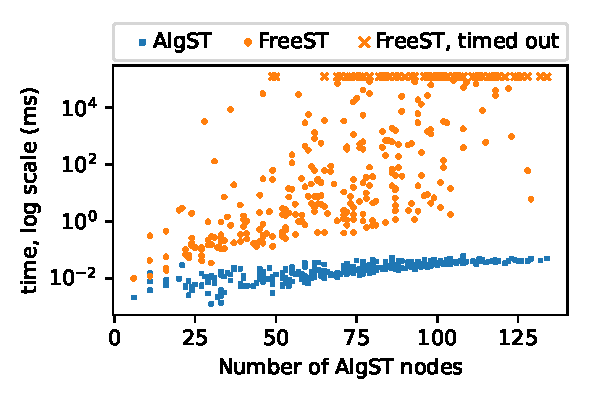
\includegraphics[width=\linewidth]{img/fig-pos.pdf}
    \caption{equivalent test cases}
    \label{fig:time-positiv}
  \end{subfigure}%
  \begin{subfigure}{.5\textwidth}
    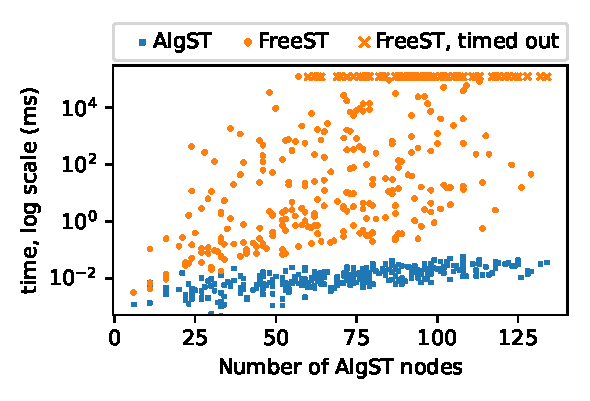
\includegraphics[width=\linewidth]{img/fig-neg.pdf}
    \caption{non-equivalent test cases}
    \label{fig:time-negative}
  \end{subfigure}
  \caption{Execution time of the \algst and FreeST type equivalence algorithms on the equivalent and non-equivalent test cases, represented in log scale as a function of the number of \algst nodes in the AST.}
  \label{fig:timings}
\end{figure}

%%% Local Variables:
%%% mode: latex
%%% TeX-master: "main"
%%% End:

\section{Related Work}
\label{sec:related}

This survey of related work concentrates on binary session types and their
treatment of recursion. Many works in the area concentrate on different aspects
and treat recursion informally as an add-on. In particular, the early work of
\citet{DBLP:conf/parle/TakeuchiHK94,DBLP:conf/concur/Honda93} did not consider
recursive types.
%
The school of session types that takes its foundations from the
sequent calculus for dual intuitionistic logic
\cite{DBLP:conf/concur/CairesP10,DBLP:journals/mscs/CairesPT16}
initially focuses on finite behaviors. While
recursion would break the logical consistency of their system, they
consider dependently typed variants that include replication
\cite{DBLP:conf/cpp/PfenningCT11}. 

\smallskip
\emph{Session type systems with recursion.}
Generally, recursive types come in two flavors, equirecursive and
isorecursive \cite{DBLP:conf/lics/AbadiF96}, and the impact of
these different approaches on type checking is well-studied
\cite{DBLP:books/daglib/0005958}. They have been found to be equally 
expressive \cite{DBLP:journals/pacmpl/PatrignaniMD21}. Most
session type systems in the literature support equirecursive session
types restricted to tail recursion and treat them informally.

Recursive types have first been introduced to session types by
\citet{DBLP:conf/esop/HondaVK98} in the context of $\pi$-calculus. Their
system relies on equirecursion and is syntactically restricted to
tail recursion.
\citet{DBLP:conf/esop/GayH99,DBLP:journals/acta/GayH05} study
subtyping in the same setting using a coinductive definition. 
% They
% define an algorithm for subtyping and develop a sound type checker.
% Most subsequent work refers to this treatment and the algorithm
% extends to their setting.
%
\citet{DBLP:conf/ppdp/CastagnaDGP09} consider recursive session types
as infinite regular trees. Their types are tagless in the sense that
choices are made according to the set of accepted values and the viability
of the continuation.
%
The functional session type calculus of
\citet{DBLP:journals/jfp/GayV10} includes subtyping and equirecursive
types, but the latter are restricted to tail-recursive session types.
%
Fundamentals of session types \cite{DBLP:journals/iandc/Vasconcelos12}
proposes a range of $\pi$-calculus-based systems with increasing
complexity. One particular focus is the treatment of replication and unrestricted
channel ends, which requires recursive types. In this work, recursive
types are modeled by infinite regular trees, represented using the
familiar $\mu$ notation with contractive, tail recursive bodies.
% no subtyping

\citet{DBLP:conf/esop/ToninhoCP13} extend the linear-logic based line
of work and focus on the combination of functions and processes
including recursive processes and consequently recursive
types for processes and functions. The examples indicate the equirecursive variant.
Apparently, there is no restriction in the use of recursion and
sequencing is implemented using the tensor $\otimes$.
% Saving some space; also I do not quite understand the restriction
% However, linearity stops them to write a type
% like $\alpha\otimes\alpha$ when $\alpha$ is a session type:
% operationally, it would mean that a process spawns a copy of itself,
% which is not possible in their system (unless via replication, which
% is modeled with a different logical connective).
%
\citet{DBLP:conf/tgc/ToninhoCP14} cover a different aspect of
equirecursion. They consider corecursive protocol definitions and
analyze their productivity. The main question they pursue is when a
corecursive protocol produces the next value after finitely many
internal steps.
%
SILL \cite{DBLP:conf/fossacs/PfenningG15} is a process-based language design that
integrates linear and affine types as well as synchronous and
asynchronous communication. It builds directly on the linear logic interpretation of session
types. Its examples make use of polymorphism and equirecursive types in the form of tail
recursive type equations, neither of which are reflected in the type
theoretical presentation.
% Subsequent work on manifest sharing also
% takes polymorphism and equirecursion for granted \cite{DBLP:journals/pacmpl/BalzerP17}.
%
\citet{DBLP:conf/concur/BartolettiSZ14} offer a semantic analysis of
session types on the basis of labeled transition systems. Their
system features equirecursion in tail position.


% \begin{itemize}
% \item X equi, regular, pi-calculus \cite{DBLP:conf/esop/HondaVK98},
%   first with recursion?
% \item X equi, regular, pi-calculus, subtyping \cite{DBLP:conf/esop/GayH99}
% \item X equi, regular \cite{DBLP:journals/jfp/GayV10}
% \item X equi, regular, pi-calculus ``fundamentals''
%   \cite{DBLP:journals/iandc/Vasconcelos12}
% \item X equi, regular, process and functional
%   \cite{DBLP:conf/esop/ToninhoCP13}
% \item X equiv, regular, process \cite{DBLP:conf/tgc/ToninhoCP14}: this
%   is really corecursion, focuses on productivity where a process is
%   guaranteed to take finitely many internal steps and then engages in
%   the next communication
% \item equi, regular, pi-calculus \cite{DBLP:journals/corr/Dardha14}
%   (focus on encoding of recursive sessions in recursive linear pi
%   calculus, duality and recursion)
% \item X equi, regular, lts \cite{DBLP:conf/concur/BartolettiSZ14}
% \item X SILL: implicit use of regular equirecursion \cite{DBLP:conf/fossacs/PfenningG15}
% \item X iso(?), regular \cite{DBLP:conf/icfp/LindleyM16}
% \item X equi, regular \cite{DBLP:journals/pacmpl/BalzerP17}
% \item equi, regular \cite{lindley17:_light_funct_session_types}
% \item Padovani's FUSE with OCaml implementation. 
% \item equi, regular \cite{DBLP:conf/esop/VasconcelosCAM20}
% \item infinite regular trees \cite{DBLP:journals/pacmpl/CicconeP22}
% \item X defined by different kinds of systems of equations \cite{DBLP:conf/fossacs/GayPV22}
% \end{itemize}


\citet{DBLP:conf/icfp/LindleyM16} define two
functional session type systems with recursion, $\mu$GV and $\mu$CP, and show that
they are related by typing- and semantics-preserving translations. So
we only compare to $\mu$GV in the following. $\mu$GV is based on
a simply-typed linear lambda calculus extended with notions of recursion and
corecursion. These are defined as least and greatest (respectively) fixed points of
strictly positive functors --- analogous to a logically
meaningful version of algebraic (co-) datatypes --- with generic fold and
unfold operators. Finally, they lift this isorecursive treatment of
recursive data to the level of session types by encoding branching and
recursion, mapping the corresponding data functors over session
types and wrapping them in promises.
We conclude that $\mu$GV features session types with isorecursion and
that it could be used to encode the simply-typed fragment of \algst,
but without parameterized data types and without the over
direction. Where $\mu$GV uses promises (i.e., a separate channel) to encode the argument to the
fold of the recursive type (i.e., the constructor arguments of an
algebraic datatype), \algst transmits the body of the fold on the same
channel, thus avoiding the overhead of channel creation.
Moreover, $\mu$GV is mainly a theoretical contribution
whereas a full implementation of \algst is available.

\smallskip
\emph{Context-free and nested session type systems.}
\citet{DBLP:conf/icfp/ThiemannV16} proposed
context-free session types to enable the type-safe encoding of
non-regular protocols like the serialization of tree structures or the
stack protocol from the introduction without encurring the overhead of
session initiation. They changed the asymmetric structure of the
traditional session type syntax $\TIn TS$ and $\TOut TS$, where an
item of type $\typec T$ is communicated and the session continues with
$\typec S$,
to a symmetric structure where session types can be built from the
atomic transmissions, $\TGIn T$ and $\TGOut T$, choice and branching,
$\TChoice{S_1}{S_2}$ and $\TBranch{S_1}{S_2}$,  and a monoidal sequential
composition operator $\TSeq{S_1}{S_2}$ with unit $\TSkip$. 
% For example, here
% is the type for transmitting a binary tree
% (\cf \cref{sec:algebr-datatyp-as}) in their system:
% $ \typec{\mu X.} \TChoice{\TGOut\TInt}{(\TSeq XX)}$.
This design,
together with equirecursive sessions, leads to a number of technical
problems. First, types come with a non-trivial equational theory:
sequential composition forms a monoid with unit $\TSkip$ and it
distributes over choice and branching. Second, polymorphic recursion
is needed as a recursive call may have to be instantiated with
different continuation sessions. Third, the interaction between
equirecursion and the omission of the restriction to tail recursion
gives rise to a difficult, but decidable, type equivalence relation.
%
Subsequent work investigated tractable algorithms for type
equivalence
\cite{DBLP:journals/corr/abs-1904-01284,DBLP:conf/tacas/AlmeidaMV20}.
\citet{DBLP:journals/corr/abs-2106-06658} integrate context-free
session types with explicit polymorphism in the style of
System~F. Recent work extends this approach with higher-order types
\cite{DBLP:journals/corr/abs-2203-12877}.

\citet{DBLP:conf/esop/Padovani17,DBLP:journals/toplas/Padovani19}
proposes a different approach to context-free session types embodied
in a functional session calculus called \fuse. This calculus uses the
type language of context-free session types, but
sidesteps the problems with the sequencing operator and type
equivalence by introducing a resumption operator $\{e\}_c$ that
deconstructs a sequence of sessions on channel $c :
\TSeq{S_1}{S_2}$. It does so by retyping the channel to $c : \typec{S_1}$ for
evaluating $e$, which must return the same channel after finishing
$\typec{S_1}$.
More formally, the resumption obeys some kind of frame rule: if  $c :
\typec{S_1} \vdash e : \typec{T \times \TOne}$, then
$c : \TSeq{S_1}{S_2} \vdash \{e\}_c : \typec{T \times S_2}$. The
resumption temporarily removes the continuation
$\typec{S_2}$ from the session type and sticks it back on
afterwards. The type system has means to make sure that the channel returned by $e$ is
identical to $c$, which is required for soundness. The type $\TOne$
does not signify the end of the session, but rather that some known
part of the session has been processed and the session will be
continued in the context (of the resumption).
%
The management of the choice and branch operations is very close to
\algst. \fuse implements choice by transmitting the constructor tag in
a variant type that selects the different continuations. Its branch
operator matches on the received constructor and thus selects the
desired continuation. However, the handling of protocol constructors
in \algst includes the construction of the continuation type from the
types and directions given in the protocol declaration. \fuse has no
equivalent to a protocol declaration nor to the type operator
\lstinline+-+ to swap the direction of a transmission.
%
\citet{DBLP:journals/toplas/Padovani19} implements
\fuse in OCaml and demonstrates that context-free session types
are amenable to type inference, if the programmer helps with judicious
placement of resumptions. Support for equirecursion is already built into  OCaml's type inference
engine. It is also shown that subtyping is undecidable.

\citet{DBLP:conf/esop/DasDMP21} propose the metatheory of 
nested session types featuring parametrized definitions of session types
with nested polymorphic recursion. 
At first glance, the nested session type 
$\syntax{List}[\alpha] = \oplus\{\syntax{nil}\colon \syntax{end}, \syntax{cons}\colon \alpha \otimes \syntax{List}[\alpha]\}$
is very similar to the algebraic protocol
$\protocolk\ \TPApp{\syntax{List}}\alpha = \termc{\syntax{Nil}}\ |\
\termc{\syntax{Cons}}\ \alpha\ (\typec{\syntax{List}}\ \alpha)$, but
there are significant differences. On the
algebraic side, we can materialize the \typec{\syntax{List}} protocol in a type  
that sends or receives a list of integers, while the nested type $\syntax{List}$ is 
already committed to a concrete direction.
%
Although type nesting enables to capture the modularity characterizing 
algebraic sessions, there are several features that distinguish AlgST from 
nested session types:
Das et al. propose a structural and equirecursive, rather than a
nominal, view of type definitions, and interpret types coinductively, rather than inductively.
These features have significant impact on the complexity of the 
equivalence problem for nested session types and on its implementation:
Das et al. present a sound but incomplete algorithm for type equivalence.
By considering a nominal interpretation of algebraic session types, we reduced the 
complexity of the equivalence problem from 
doubly-exponential~\cite{DBLP:conf/esop/DasDMP21} to 
linear and designed a sound and complete algorithm to verify type
equivalence. The examples in section~2 of
\citet{DBLP:conf/esop/DasDMP21} translate into \algst and type check with our implementation.

\citet{DBLP:conf/fossacs/GayPV22} consider equirecursive protocols
defined by different kinds of systems of equations (with and without
parameters). Imposing different restrictions on the parameterization
yields different classes of protocols with decision problems for type
equivalence ranging from polytime to undecidable. Their largest
decidable class of pushdown session types is shown to be equivalent to
nested session types, which we can model with \algst.

Compared to all competiting systems \cite{DBLP:journals/pacmpl/ThiemannV20,DBLP:journals/corr/abs-2106-06658,DBLP:journals/toplas/Padovani19,DBLP:conf/esop/DasDMP21}, \algst's materialization and
directional operators are unique. These
operators enable the construction of protocols without committing to a
particular direction. 

%%% MPST:
%%% (equi, regular) Less is more: multiparty session types revisited

% \paragraph{Protocol composition}
% \label{sec:protocol-composition}

% \citet{DBLP:journals/corr/abs-2203-02461} define a notion of protocol
% composition which interleaves two or more protocols. To
% restrict this liberal approach to sensible interleavings, protocols
% are extended with an assertion language that specifies safe
% interleavings. Interleaving composition is complementary to our
% modular approach to protocol construction: we combine subprotocols
% rather than interleave them.

\smallskip
\emph{Linear and unrestricted types.}
Our 
%formal 
calculus is mostly linear, except that we
%. The only exception we make is to
allow unrestricted bindings for recursive functions, which would be
rendered useless otherwise. 
%On the other hand, we want to speak about
%recursive protocols, so we felt like recursive functions are needed in
%the formal development. 
Our implementation goes well beyond that in
allowing fully fledged unrestricted computations besides ensuring that
session typed channels are treated linearly.
% That said, all related work is closer to our implementation than to
% the formal calculus.
%
There is some work on recursion and linearity in the context of lambda calculus
\cite{DBLP:journals/lisp/AlvesFFM10}
%. This work 
adding iterators on
linear natural numbers to the calculus, thereby avoiding the need for
a rule like {\rulenameexpUVar}.
%, which we need to bind the recursive function to a name.

System F\degree~\cite{DBLP:conf/tldi/MazurakZZ10}
extends System F with kinds to integrate polymorphism with linear and
unrestricted types. This work serves as a blueprint for much
subsequent work in this area including LFST and FreeST (see below), as well as our
implemented language.
They categorize all objects, including functions, into one-use or
many-use resources. This style can be traced back to 
\citet{walker:substructural-type-systems}. 
% One example in the paper applies the language to protocols built with
% linear capabilities, reminiscent of session types.
%
LFST \cite{lindley17:_light_funct_session_types} formalizes the
session type system of Links, which features a mix of linear and
unrestricted types, embedding a standard functional programming
language. The substructural behavior of types is specified by a
sophisticated kind structure.  The kinding used in our implementation
is inspired by LFST, though LFST has additional kinds to describe row
types that we do not support.
%
\citet{DBLP:journals/corr/abs-2106-06658}
consider an integration of context-free session types with
System~F. Their type system includes a kinding discipline that manages
linear and unrestricted versions of ordinary types and
message types (possible payloads for the send and receive
operations). Our implemented system extends the kind structure in a
similar way.

Linear Haskell (LH) \cite{DBLP:journals/pacmpl/BernardyBNJS18}
is a proposal to integrate linear types with stock functional
programming. While the work discussed so far characterizes resources,
LH supports the lollipop type $S \multimap T$ which classifies
functions that use their argument exactly once. Originally, LH forced
the programmer to allocate resources using continuations. This restriction
has been fixed in subsequent work \cite{DBLP:journals/pacmpl/SpiwackKBWE22}.
%
There is further work on integrating linear and dependent types (e.g.,
\cite{DBLP:conf/popl/KrishnaswamiPB15}) which relies on
bifurcating the language in two calculi connected by an adjunction.

% We believe that \algst definitions that do not make
% significant use of negation on protocols

%%% Local Variables:
%%% mode: latex
%%% TeX-master: "main"
%%% End:


% \paragraph{Further work on duality and recursion}

% The problem with duality and recursion mentioned in
% \cref{sec:what-about-inter} was first reported by
% \citet{DBLP:journals/corr/abs-1202-2086}. % (Bono and Padovani, 2012)
% It was further studied and fixed by \citet{BernardiH14, BernardiH16}. %(Bernardi Hennessy, 2014)
% \citet{DBLP:conf/icfp/LindleyM16} propose a different solution using
% covariables. A recent study closes the matter \cite{DBLP:journals/corr/abs-2004-01322}.



% (Gay and Thiemann and Vasconcelos, 2020)
% \cite{DBLP:journals/corr/Dardha14}

% \paragraph{Not recursive}
% \begin{itemize}
% \item Towards Races in Linear Logic (Kokke, Morris, Wadler)
% \item Exceptional GV (Fowler etal)
% \item Gradual Session Types 
% \item Bernardo Toninho, Nobuko Yoshida: Interconnectability of
%   Session-Based Logical Processes
% \item Bernardo Toninho, Nobuko Yoshida: Depending on Session-Typed
%   Processes
% \item Sam Lindley, J. Garrett Morris: Embedding session types in Haskell.
% \item Lindley and Morris, Semantics for Propositions as Sessions, ESOP
%   2015
% \item Mazurak and Zdancewic, Lolliproc: to Concurrency from Classical
% Linear Logic via Curry-Howard and Control, ICFP 2010
% \item Perez and Caires and Pfenning and Toninho, Linear logical
%   relations and observational equivalences for session-based
%   concurrency, I\&C 2014
% \item Riccardo Pucella and Jesse A. Tov, Haskell Session Types with
%   (Almost) No Class, 2008
% \item X An interaction-based language and its typing system
% Kaku Takeuchi, Kohei Honda \& Makoto Kubo, PARLE 1994 \cite{DBLP:conf/parle/TakeuchiHK94}
% \end{itemize}

%%% Local Variables:
%%% mode: latex
%%% TeX-master: "main"
%%% End:

\section{Conclusion}
\label{sec:conclusion}

Algebraic protocols combine naming and recursion with choice %/branch
and sequence type constructors known from session types. Like algebraic datatypes,
they offer parameterization and mutual recursion. Unlike previous work on
session types, algebraic
protocols do not commit to a particular direction of communication,
even if direction reversal can be specified at the type level. Algebraic protocols
and session types subsume the expressive power of context-free and nested
session type systems while reducing the complexity of type checking
from doubly-exponential to linear time.

%%% Local Variables:
%%% mode: latex
%%% TeX-master: "main"
%%% End:


\section*{Acknowledgements}
We thank the reviewers for their suggestions that greatly
contributed to a more solid version of the paper. Support for this research was provided by the
Fundação para a Ciência e a Tecnologia through project SafeSessions, ref.\
PTDC/CCI-COM/6453/2020, and the LASIGE Research Unit, ref.\ UIDB/00408/2020 and
ref.\ UIDP/00408/2020, and by the COST Action EuroProofNet (CA20111).

\section*{Software Availability}
\label{sec:artifact}

The proposed system and implementation are publicly available as an artifact \cite{artifact}. The interested reader can follow the steps in the artifact documentation to set up a pre-built docker image or a self-built docker image. Besides the implementation of the type checker and the interpreter, we provide programs for all the examples in the paper and examples that establish a comparison with related work \cite{DBLP:conf/esop/DasDMP21,DBLP:conf/icfp/ThiemannV16}. In the artifact, the reader can also find instructions on how to reproduce our benchmarking results for type equivalence.

%%% Local Variables:
%%% mode: latex
%%% TeX-master: "main"
%%% End:

% \section{Questions}
\label{sec:questions}

Proposition: Every nominal session typed program can be translated into a
context-free session typed program.

Conjecture: Every regular session typed program (without subtyping)
can be translated into a nominal session typed program.

This is non-trivial because regular session types
have more liberal, structural matching of recursive types. To this
end, one would have to define a normal form for recursive session
types such that type matching is decided by comparing normal
forms. The normal form can be rendered directly as a nominal type.

Conjecture: There is a context-free session-typed program that cannot
be translated to a nominal session typed program.

%%% Local Variables:
%%% mode: latex
%%% TeX-master: "main"
%%% End:

\bibliographystyle{plainnat}
\bibliography{biblio}

\newpage
\appendix
\section{Frequently Asked Questions}
\label{sec:freq-asked-quest}

\subsection{Session types vs.\ protocol types}
\label{sec:what-diff-betw-1}
 A session type can be assigned to a channel end to describe
the entire communication behavior of this channel up to its closing. Thus, a
session type classifies a run-time value, namely a channel end.
A protocol type does not correspond to any run-time value.  It
describes composable behavior for bidirectional communication. A protocol
type becomes part of a session type by binding it to a particular
direction with the $!$ and $?$ operators.

In a sense, a protocol type describes a composable part of a
communication protocol or the difference between two session
types. This view is emphasized by our pervasive use of channel passing
style. 

\subsection{Negated recursion}
\label{sec:what-about-protocol}
It is possible to define an algebraic protocol that negates the polarity of its recursive use.
Such a protocol is fine, though unusual as it changes
direction with every unfolding of the recursion. Here is an example:
\begin{lstlisting}
protocol Flipper = Flipper -Int -Flipper
\end{lstlisting}
A server for \lstinline+Flipper+ can be implemented with a pair of
mutually recursive functions or even with just one function:
\begin{lstlisting}
flipper : !Flipper.EndT -> Unit
flipper c = let c = select Flipper [EndT] c in
            let (x, c) = receive [Int, ?Flipper.EndT] c in
	    match c with {
	      Flipper c -> send [Int, !Flipper.EndT] x c |> flipper }
\end{lstlisting}

\subsection{Mutual recursion}
\label{sec:do-you-support}
Mutually recursive protocols pose no problem. In general, the server
would be implemented by mutually recursive functions.
% In our recoding of the example in
% \cref{sec:what-about-protocol}, a single recursive function is sufficient:
% \begin{lstlisting}
% protocol Flip = Flip -Int Flop
% protocol Flop = Flop Int Flip

% flipflop : !Flip.End -> End
% flipflop c = let c = select Flip [End] c in
%             let (x, c) = receive [Int, !Flop.End] c in
% 	    select Flop [End] c
% 	    |> send [Int, !Flip.End] x []
%             |> flipflop
% \end{lstlisting}
\begin{lstlisting}
protocol Flip = Flip -Int Flop
protocol Flop = Flop Int Flip

flip : !Flip.EndT -> Unit
flip c = select Flip [EndT] c |> receive [Int, !Flop.EndT] |> flop

flop : (Int, !Flop.EndT) -> Unit
flop p = let (x, c) = p in
         select Flop [EndT] c |> send [Int, !Flip.EndT] x |> flip
\end{lstlisting}
\subsection{Duality vs.\ polarities}
\label{sec:what-diff-betw}
The \lstinline+Dual+ operator works on \emph{session types} and it inverts
the direction of communication from the outside. Intuitively, the
\lstinline+Dual+ operator traverses the spine of a session type and
flips all $!$ to $?$ and vice versa. It does \textbf{not} enter the
type of the message ``payload''. For example (with $\typec T$ the
payload type and $\typec S$ the continuation session):
\begin{align*}
  \TDual{(\TIn TS)} &\equiv \TOut T{\TDual S} &   \TDual{(\TOut TS)} &\equiv \TIn T{\TDual S}
\end{align*}
In contrast, the polarity operator \lstinline+-+ works on
\emph{protocol types} and inverts the direction of communication from
the inside. This inversion happens at the boundary where a protocol
type $\proto$ is turned into a payload type for a session:
\begin{align*}
  \TIn {(\TMinus P)}S &\equiv \TOut P S &\TOut {(\TMinus P)}S &\equiv \TIn P S
\end{align*}
The soundness of the type system guarantees that the direction of communication is
finally settled by the time we get to a primitive sending or receiving operation.

Like \lstinline+Dual+, the \lstinline+-+ operator is involutory:
\begin{align*}
  \TDual{(\TDual{S})} &\equiv \typec{S} &   \TMinus{(\TMinus T)} &\equiv \typec{T}
\end{align*}

\subsection{Recursion and duality}
\label{sec:what-about-inter}
\citet{BernardiH14,BernardiH16} discovered a problem in the interaction
between duality and recursive session types, which is exposed most
concisely by the recursive type $\typec{T =\mu X. !X.X}$.
The dual of this type is $\TDual{(\mu X. !X.X)} = \typec{\mu
  X.\TIn{(\mu X. !X.X)}X}$, which can be seen by dualizing the type's
expansion
\begin{equation*}
  \TDual{(\mu X. !X.X)} = \TDual{(!(\mu X.!X.X). (\mu X.!X.X))} \\
                        = \TIn{(\mu X.!X.X)}{\TDual{(\mu X.!X.X)}}
\end{equation*}
Using equations we could define the type $\typec T$ by $\typec{T = \TOut{T}T}$.
Translated to algebraic session types, the protocol underlying $\typec T$ is as follows:
\begin{lstlisting}
protocol X = Mu T X
type T = !X.EndT

selectMu : T -> !T.T
selectMu c = select Mu [EndT] c

dualT : Dual T -> ?X.EndT
dualT c = c

matchMu : Dual T -> ?T.(Dual T)
matchMu c' = match c' with { Mu c' -> c' }
\end{lstlisting}
This behavior matches exactly the outcome for $\typec T$ according to
\citet{BernardiH16}. The function \lstinline+selectMu+ performs the
unfolding of $\typec T$ whereas \lstinline+matchMu+ performs the
unfolding of $\TDual T$. The type of the identity function
\lstinline+dualT+ shows that \lstinline+Dual T = ?X.EndT+. 

\subsection{Efficiency of generic servers}
\label{sec:are-generic-servers}
In \cref{sec:toolb-gener-serv}, we explore an example with generic servers 
to showcase the expressivity of the proposed parametric protocols.
The example has a significant overhead as there are many tagging
operations compared to a manually crafted version.  

The present work is a first step and does not offer a solution
supported by formal theorems. But, let us call a protocol $\proto$
\emph{tagless} if it is non-recursive and declares a  single
constructor tag $\constr\ T_1\dots T_n$. In analogy to Haskell's
\texttt{newtype}, an implementation can reduce the
run-time cost of a tagless protocol to zero by omitting the select and
match operations. 

\subsection{Equirecursive vs. isorecursive session types}
\label{sec:this-session-types}
Most work on session types is using equirecursive types for two reasons. One is historic:
\citet{DBLP:conf/esop/GayH99,DBLP:journals/acta/GayH05} were the first
to study coinductively defined relations on (tail-) recursive session types. They defined the (by now)
standard notion of subtyping and showed that it is
decidable. Subsequent work has built on top of their results. The
other reason is that ``The equirecursive interpretation of a session type guarantees that no
message is required for the unfolding of a recursive type.'' (\citet{DBLP:journals/pacmpl/BalzerP17})

Algebraic protocols conflate the unfolding of the recursion with
the branching, just like algebraic datatypes do.
For protocols that have finite runs, algebraic protocol do not cause extra messages.
As such protocols use recursion guarded by branching, a
message to decide the branching is needed anyway.

The protocol \lstinline+Stream a+ in \cref{sec:param-prot} does cause
extra messages as it (roughly) corresponds to an isorecursive reading of the type $\mu X. !a.X$.

\subsection{Subtyping, type classes, type inference}
\label{sec:can-you-do}

Subtyping is undecidable for context-free session types
\cite{DBLP:journals/toplas/Padovani19}. However, as \algst's session
typing relies mostly on nominal types, there is scope for decidable
subtyping. We have a concrete proposal, but it is not implemented
and its metatheory has not been checked, yet.

The types \lstinline+Send a+ and \lstinline+Recv a+ for sending and
receiving data of type \lstinline+a+ in \cref{sec:transm-param-data}
look like types for a dictionary in a language with type classes or
traits
\cite{DBLP:journals/toplas/HallHJW96,steve18:_rust_progr_languag}. 
%
In future work we plan to explore the addition of implicit arguments as
in Scala \cite{DBLP:journals/pacmpl/OderskyBLBMS18}. 

Type inference is future work.

\subsection{Settling of direction}
\label{sec:settling-direction}
It might be confusing to see a type like $\TIn TS$ and $\TOut TS$, but
with the possibility that the direction changes later on. However,
this behavior is completely predictable. As long as $\typec T$ is a
protocol type variable  $\alpha : \kindp$, the direction can change
because $\alpha$ could be substituted by some protocol $\TMinus {T'}$. 
As soon as $\typec T$ is an ordinary type of kind $\kindt$ (even if
$\typec T$ is a variable), the direction is fixed. For example, in the
type of primitive send
\lstinline+forall(a:M). forall(s:S).  a -> !a.s -> s+, the payload type
\lstinline+a+ has kind $\kindm$, so the direction is fixed. \\

%%% Local Variables:
%%% mode: latex
%%% TeX-master: "main"
%%% End:

\section{A Toolbox for Generic Servers}
\label{sec:toolb-gener-serv-1}


Analogously to the \lstinline+Stream+ protocol, we can define a protocol
and a generic server for finite repetion of a subsidiary protocol:
\begin{lstlisting}
protocol Repeat x = More x (Repeat x) | Quit

repeat : forall(p:P). Service p -> Service (Repeat p)
repeat [p] serveP [s] c = match c of {
  Quit c -> c,
  More c -> serveP [?Repeat p.s] c |> repeat [p] serveP [s]
}
\end{lstlisting}
This protocol may then be used similarly to  \lstinline+Stream+:
\begin{lstlisting}
repeatArith = repeat [Arith] serveArith
\end{lstlisting}
We can define an active version that offers the subprotocol $n$ times
and use that with \lstinline+Arith+, too:
\begin{lstlisting}
repeatActive : Int -> forall(p:P). Service p -> Service -(Repeat -p)
repeatActiveArith : Int -> Service -(Repeat -Arith)
\end{lstlisting}
While the implementation is straightforward, the astute reader might
ask why we provide the negative parameter to \lstinline+Service+ in
\lstinline+Service -(Repeat -p)+. In particular, could we not use the
\lstinline+Dual+ operator to switch the direction of the service?

To see the problem with this proposal, let's expand the two candidates:
\begin{lstlisting}
Dual (Service (Repeat -p)) = Dual (forall(s:S). ?Repeat -p.s -> s)
\end{lstlisting}
This proposal is doomed because the use of \lstinline+Dual+ on the
right side is not well-kinded, as neither the
universal type nor the function types are session types in our
system.
% Even applying \lstinline+Dual (?Repeat -p. s)+ results in
% \lstinline+!Repeat -p. Dual s+ with a dualized continuation.

\begin{lstlisting}
Service -(Repeat -p) = forall(s:S). ?- (Repeat -p). s -> s
                     = forall(s:S). !Repeat -p. s -> s
\end{lstlisting}
The negative parameter swaps the receiving operator in
\lstinline+Service+ to sending with surgical precision.


%%% Local Variables:
%%% mode: latex
%%% TeX-master: "main"
%%% End:

\section{Proofs for Types}

\begin{example}
  We generalize the example from the introduction to a
  parametric stack protocol.
\begin{lstlisting}
protocol Stack a = Pop -a | Push a (Stack a) (Stack a)
\end{lstlisting}
  We set  $ \Delta = \types{Neg} : \kindp \to \kindp, \types{a} :
  \kindp$ and obtain
  the straightforward derivation
  \begin{mathpar}
    \inferrule*{
      \inferrule*
      {\inferrule*
      {\typeSynth{ \types{a} }{\kindp}}
      {\typeAgainst{ \types{a} }{\kindp}}}
      {\typeAgainst{ \types{-a} }{\kindp}} \\
      \inferrule*
      {\typeSynth{ \types{a} }{\kindp}}
      {\typeAgainst{ \types{a} }{\kindp}} \\
      \inferrule*
      {\inferrule*
        {\types{Stack} : {\kindp} \to \kindp \in \Delta \\
          \inferrule*
          {\typeSynth{\types{a}}{\kindp}}
          {\typeAgainst{\types{a}}{\kindp}}}
        {\typeSynth{ \types{Stack~a}}{\kindp}}}
      {\typeAgainst{ \types{Stack~a}}{\kindp}}
    }
    {
      \typeSynth[]{ \types{Stack} }{\kindp \to \kindp}
    }
  \end{mathpar}
  The three subderivations correspond to the arguments of the protocol
  constructors. We conclude that the definition of the protocol 
  \lstinline+Stack a+ is well-formed.
\end{example}

\begin{lemma}[Properties of the materialization and directional operators]\
  \label{lem:ops-dual}
  \begin{enumerate}
    \item\label{it:dual-norm} $\isConv{\TDual{(\tosession TS)}}{\tosession{\polarizedparam{-}{T}}{\TDual{S}}}\kinds$
    \item\label{it:plus-minus} $\polarizedparam{-}{\polarizedparam{+}{T}} = \polarizedparam{-}{T}$
    \item\label{it:minus-minus} $\polarizedparam{-}{\polarizedparam{-}{T}} = \polarizedparam{+}{T}$
  \end{enumerate}
\end{lemma}
\begin{proof}\
  \begin{enumerate}
  \item By case analysis on the definition of the
    $\tosessionop$ operator (\cref{fig:type-polarized-operator}).

    Case $\typec T = \pneg U $.
    %$\isConv{\TDual{(\tosession {-T}S)}}{\tosession{\polarizedparam{-}{-T}}{\TDual{S}}}\kinds$.
    Since $\tosession {\pneg U}S = \TIn{U}{S}$, rule \rulenametconvDualInM gives
    $\isConv{\TDual{(\tosession {\pneg U}S)}}{\TOut{U}{\TDual S}}\kinds$. Observing that
    $\polarizedparam{-}{-U}=\polarizedparam{+}{U}=\typec U$ we conclude that
    $\tosession{\polarizedparam{-}{\pneg U}}{\TDual{S}}=\TOut{U}{\TDual S}$.

    Case $\typec T \neq \pneg U $
    %$\isConv{\TDual{(\tosession {T}S)}}{\tosession{\polarizedparam{-}{T}}{\TDual{S}}}\kinds$.
    Since $\tosession {T}S = \TOut{T}{S}$, rule \rulenametconvDualOutM gives
    $\isConv{\TDual{(\tosession {T}S)}}{\TIn{T}{\TDual S}}\kinds$. Conclude observing
    that $\polarizedparam{-}{T}=\typec{-T}$.
    \item The proof follows by case analysis on the definition of the directional operators.

    Case $\typec T = \pneg U $. We have:
    $\polarizedparam{-}{\polarizedparam{+}{\pneg U}} = \polarizedparam{-}{\polarizedparam{-}{U}}
    = \polarizedparam{-}{\pneg{U}}$.

    Case $\typec T \neq \pneg U $. We have:
    $\polarizedparam{-}{\polarizedparam{+}{T}} = \polarizedparam{-}{T}$.

    \item The proof follows by case analysis on the definition of the directional operators.

    Case $\typec T = \pneg U $. We have:
    $\polarizedparam{-}{\polarizedparam{-}{\pneg U}} = \polarizedparam{-}{\polarizedparam{+}{U}}
    = \polarizedparam{-}{U} = \pneg U = \polarizedparam{+}{\pneg U}$.

    Case $\typec T \neq \pneg U $. We have:
    $\polarizedparam{-}{\polarizedparam{-}{T}} = \polarizedparam{-}{\pneg T}= \polarizedparam{+}{T}$.
  \end{enumerate}
\end{proof}

\begin{lemma}[Agreement for type conversion]
  \label{it:agreement-type-conv}
  If $\isConv T U \kind$, then $\typeAgainst T \kind$ and
  $\typeAgainst U \kind$.
\end{lemma}
\begin{proof}
  By rule induction on the hypothesis.
\end{proof}


We start by specifying the syntax of types in normal form. Normal forms for well-formed types
are $\typec{Q}$ as defined by the following grammar:
%
\begin{align*}
  \typec{Q} &\grmeq \typec{R} \grmor \pneg{R}
  \\
  \typec{R} &\grmeq
  % functional types
  \TUnit \grmor \TFun[]{R}{R} \grmor \TPair{R}{R} \grmor
  \TForall \alpha \kind {R} \grmor \typec\alpha
  % session types
  \grmor \TIn{R}{R} \grmor \TOut{R}{R}
  \grmor \TEndW \grmor \TEndT  \grmor
  \TDual{\alpha}
  % protocol and data types
  \grmor \TPApp \proto {\overline{Q}}
\end{align*}


\begin{proposition}[Kind preservation]
  ~\label{lemma:kind-preservation}
  \begin{enumerate}
  \item For all $\typeSynth T\kind$,  $\isConv{\Normal[+] T}T\kind$.
  \item For all $\typeSynth T\kinds$,  $\isConv{\Normal[-] T}{\TDual T}\kinds$.
  \end{enumerate}
\end{proposition}
\begin{proof}
  See Agda development \texttt{nf-sound+} and \texttt{nf-sound-}.
\end{proof}

\begin{proof}[Proof of \cref{thm:soundness-type-equiv} (Soundness)]
  \Cref{it:soundness-type-equiv-t}. Suppose that $\Normal[+] T =_\alpha \Normal[+] U$. From
  \cref{lemma:kind-preservation}, we have  $\isConv{\Normal[+]
    T}T\kind$ and  $\isConv{\Normal[+] U}U\kind$. Conclude by symmetry
  and transitivity of conversion as type equality is in $\equiv$.
  % 
  The proof for \cref{it:soundness-type-equiv-s} is analogous.
\end{proof}

\begin{proof}[Proof of \cref{thm:completeness-type-equiv} (Completeness)]
  See Agda development \texttt{nf-complete} and \texttt{nf-complete-}.
\end{proof}

To obtain a complexity bound for the computation of a normal form,
we exploit its syntactic form.
\begin{lemma}
  \label{lemma:syntax-of-type-normal-forms}
  If $\Normal[\pm]T = \typec{T'}$, then $\typec{T'}$ is described by $\typec{Q}$.
\end{lemma}
\begin{proof}
  See Agda development \texttt{nf-normal}.
\end{proof}
\begin{proposition}
  For each $\typeSynth T\kind$,
  the worst case running time of $\Normal[\pm]T$ is in $O(|\typec{T}|)$.
\end{proposition}
\begin{proof}
  A run of $\Normal T$ visits each of the $|\typec{T}|$ nodes in the input type
  once. At each node, it either reconstructs the type from the normal forms of
  the sub-terms in $O(1)$ time, or (in the transmission rules) it applies
  polarity correction to normal forms. By
  Lemma~\ref{lemma:syntax-of-type-normal-forms}, a normal form starts with at
  most one negative polarity, so correction takes at most two steps, at cost
  $O(1)$.
\end{proof}

\begin{proof}[Proof of \cref{thm:complexity} (Time complexity of type equivalence)]
  A corollary of \cref{lemma:syntax-of-type-normal-forms}.
\end{proof}

%%% Local Variables:
%%% mode: latex
%%% TeX-master: "main"
%%% End:

\section{Proofs for expressions and processes}
\label{sec:appendix-exps-procs}
\label{sec:proofs}

% In this section we present examples and the proofs of the main results 
% of our work, along with some auxiliary lemmas. We preserve the structure 
% of the paper, split into subsections, to facilitate the mapping between 
% the supplementary material and the main document

\begin{figure}[t!]
  \declrel{Labelled transition system for expressions}{$\trans e \lambda e$}
  \begin{mathpar}
    \inferrule[Act-App]{}{\trans{\appe{(\abse{x}{T}{e})}{v}}{\beta}{\termc{e}\esubs{v}{x}}}
    
	\inferrule[Act-TApp]{}{\trans{\tappe{(\tabse{\alpha}{\kind}{v})}{T}}{\beta}{\termc{v}\tsubs{T}{\alpha}}}

	\inferrule[Act-Let]{}{\trans{\lete{x}{y}{{\paire uv}}{e}}{\beta}{\termc{e}\esubs{u}{x}\esubs{v}{y}}}

	\inferrule[Act-Let*]{}{\trans{\letu{\unitk}{e}}{\beta}{\termc{e}}}

    \inferrule[Act-Rec]{}{\trans{\appe{({\rece xTv})}
        u}{\beta}{\appe{(\termc{v}\esubs{\rece xTv}{x})}u}}

    \inferrule[Act-Fork]{}{\trans{\appe{\forkk}{v}}{\forkl{v}} \unitk}
	
	\inferrule[Act-New]{}{\trans{\tappe \newk T}{\newl xyT}{\paire xy}}

	\inferrule[Act-Rcv]{}{\trans{\appe{\tappe{\tappe \receivek T}{U}}{x}}{\receivel xv}{\paire{v}{x}}}
	
	\inferrule[Act-Send]{}{\trans{\appe{\appe{\tappe{\tappe \sendk T}{U}}{v}}{x}}{\sendl xv}{x}}
	
	\inferrule[Act-Match]{}{\trans{\matchwithe xCyeiI}{\receivel
        x{C_k}}{e_k\esubs x{y_k}}}

	\inferrule[Act-Sel]{}{\trans{\appe{\tappe{\selecte{C}}{\overline T}}{x}}{\sendl x{C}}{x}}
	
	\inferrule[Act-Wait]{}{\trans{\waite{x}}{\closel x}\unitk}

	\inferrule[Act-Term]{}{\trans{\closee{x}}{\openl x}{\unitk}}

	\inferrule[Act-AppL]{\trans{e_1}{\lambda}{e_2}}
	{\trans{\appe{e_1}{e_3}}{\lambda}{\appe{e_2}{e_3}}}
	
	\inferrule[Act-AppR]{\trans{e_1}{\lambda}{e_2}}
	{\trans{\appe{v}{e_1}}{\lambda}{\appe{v}{e_2}}}
	
	\inferrule[Act-TAppE]{\trans{e_1}{\lambda}{e_2}}
	{\trans{\tappe{e_1}T}{\lambda}{\tappe{e_2}T}}
	
	% \inferrule[Act-LetE]{\trans{e_1}{\lambda}{e_2}}{\trans{\lete xy{e_1}{e_3}}{\lambda}{\lete xy{e_2}{e_3}}}
	%
	% \inferrule[Act-LetE*]{\trans{e_1}{\lambda}{e_2}}{\trans{\letu {e_1}{e_3}}{\lambda}{\letu{e_2}{e_3}}}

	\inferrule[Act-PairL]{\trans{e_1}{\lambda}{e_2}}
	{\trans{\paire{e_1}{e_3}}{\lambda}{\paire{e_2}{e_3}}}	
	
	\inferrule[Act-PairR]{\trans{e_1}{\lambda}{e_2}}
	{\trans{\paire{v}{e_1}}{\lambda}{\paire{v}{e_2}}}

	\inferrule[Act-MatchE]{\trans{e_1}{\lambda}{e_2}}
	{\trans{\matchwithe{e_1}CxeiI}{\lambda}{\matchwithe{e_2}CxeiI}}

	\inferrule[Act-LetE]{\trans{e_1}{\lambda}{e_2}}{\trans{\lete xy{e_1}{e_3}}{\lambda}{\lete xy{e_2}{e_3}}}

	\inferrule[Act-LetE*]{\trans{e_1}{\lambda}{e_2}}{\trans{\letu {e_1}{e_3}}{\lambda}{\letu{e_2}{e_3}}}
  \end{mathpar}
  \caption{Labelled transition system for expressions}
  \label{fig:lts-exps}
\end{figure}

%%% Local Variables:
%%% mode: latex
%%% TeX-master: "main"
%%% End:


\begin{lemma}\
  \label{lem:synth-against-nf}
  \begin{enumerate}
       \item\label{it:synth-nf} If $\expSynth{\Gamma_1} eT{\Gamma_2}$ and $\isCtx[\Delta]{\Gamma_1}{\kindt}$, 
       then $\isCtx[\Delta]{\Gamma_2}{\kindt}$ and $\typec T$ is in normal form.
       \item\label{it:against-nf}  If $\expAgainst{\Gamma_1} eT{\Gamma_2}$ and $\isCtx[\Delta]{\Gamma_1}{\kindt}$
       and $\typec T$ is in normal form, then $\isCtx[\Delta]{\Gamma_2}{\kindt}$.
  \end{enumerate}
  \begin{proof}\
  \begin{enumerate}
       \item By rule induction on the first hypothesis.
       \item Using \cref{it:synth-nf} and observing that a type $\typec U$ such that 
       $\hl{\typec U \subt \typec T}$ is also in normal form.
  \end{enumerate}         
  \end{proof}
\end{lemma}

%% section 5
% \subsection{Metatheory}

\begin{figure}[t!]
    \declrel{Labelled transition system for contexts}{$\Gamma\lts{\lambda} \Gamma$\quad $\Gamma\lts{\pi} \Gamma$}
\begin{mathpar}
    \inferrule[L-Rcv]
    {\expAgainst[\Empty]{\Gamma}{v}{T}{\Empty}}
    {\transCtx{\ebind{x}{\TIn{T}{S}}}{\receivel{x}{v}}{\Gamma,\ebind{x}{S}}}
    
    \inferrule[L-Send]
    {\expAgainst[\Empty] \Gamma v T \Empty}
    {\transCtx{\Gamma, \ebind{x}{\TOut{T}{S}}}{\sendl{x}{v}}{\ebind{x}{S}}}
    
    \inferrule[L-Match]
    {\protocolsfull}
    {\transCtx{\ebind{x}{\TIn{(\TPApp \proto{\overline{U}})}{S}}}{\receivel{x}{C_k}}{\ebind{x}{\matchin[k]}}}
    
    \inferrule[L-Sel]
    {\protocolsfull}
    {\transCtx{\ebind{x}{\TOut{(\TPApp \proto{\overline{U}})}{S'}}}{\sendl{x}{C_k}}{\ebind{x}{\matchout[k]}}}
    
    \inferrule[L-Wait]{}
    {\transCtx{\ebind{x}{\TEndW}}{\closel{x}}{\Empty}}
    
    \inferrule[L-Term]{}
    {\transCtx{\ebind{x}{\TEndT}}{\openl{x}}{\Empty}}
    
    \inferrule[L-Beta]{}
    {\transCtx{\Empty}{\beta}{\Empty}}
    
    \inferrule[L-Fork]
    {\expAgainst[\Empty]{\Gamma}{v}{\TFun[]\TUnit\TUnit}{\Empty}}
    {\transCtx{\Gamma}{\forkl{v}}{\Empty}}
    
    \inferrule[L-New]{}
    {\transCtx{\Empty}{\newl xyT}{\ebind{x}{\Normal[+] T}, \ebind{y}{\Normal[-]{T}}}}
    
    \inferrule[L-Tau]{}
    {\transCtx{\Empty}{\tau}{\Empty}}
    
    \inferrule[L-OpenL]{}
    {\transCtx{\ebind{x}{\TOut{T}{S}}}{\scopel abxa}{\ebind{b}{\Normal[-]{T}},\ebind{x}{S}}}
\quad
    \inferrule[L-OpenR]{}
    {\transCtx{\ebind{x}{\TOut{T}{S}}}{\scopel abxb}{\ebind{a}{\Normal[-]{T}},\ebind{x}{S}}}
\quad
    \inferrule[L-Par]
    {\transCtx{\Gamma_1}{\pi_1}{\Gamma_3}
    \and \transCtx{\Gamma_2}{\pi_2}{\Gamma_4}}
    {\transCtx{\Gamma_1,\Gamma_2}{\parl{\pi_1}{\pi_2}}{\Gamma_3,\Gamma_4}}
\end{mathpar}
\caption{Labelled transition system for typing contexts}
\label{fig:lts-ctx}
\end{figure}
%%% Local Variables:
%%% mode: latex
%%% TeX-master: "main"
%%% End:


% \paragraph{Preliminaries} We start with some basic results.

\begin{lemma}[Properties of normalization]\
  \label{lem:norm-st}
  % Let $\typeSynth U \kind$.
  \begin{enumerate}
  \item\label{it:anti-plus} If $\typeSynth{\Normal[+] T} \kind$, then
    $\typeAgainst T \kind$.
  \item\label{it:anti-minus} If $\typeSynth{\Normal[-] T} \kind$, then
    % $\kind = \kinds$ and 
    $\typeAgainst T \kinds$.
  \item\label{it:anti-tosession} If $\typeSynth{\tosession TS} \kind$, then
    % $\kind = \kinds$ and 
    $\typeAgainst T \kindp$ and $\typeAgainst S \kinds$.
  \item\label{it:anti-pm} If $\typeSynth{\polarizedparam \pm T} \kind$,
    then $\typeAgainst T \kind$.
  \end{enumerate}
\end{lemma}
%
\begin{proof}
  The proof is by mutual induction on the various hypotheses. Most cases follow
  by a straightforward induction. We detail the case for
  $\Normal[-]{\typec{\TIn TS}} = \TFOut{\Normal[+]T}{\Normal[-]S}$.
  \Cref{it:anti-tosession} gives
  $\typeAgainst {\polarizedparam +{\Normal[+]T}} \kindp$ and
  $\typeAgainst {\Normal[-]S} \kinds$. Rule \rulenametypeSub gives
  $\typeSynth {\polarizedparam +{\Normal[+]T}} \kindp$ and
  $\typeSynth {\Normal[-]S} \kinds$. \Cref{it:anti-pm} gives
  $\typeSynth {\Normal[+]T} \kindp$. Again rule \rulenametypeSub gives
  $\typeAgainst {\Normal[+]T} \kindp$. \Cref{it:anti-plus} gives
  $\typeSynth T \kindp$. Once again, rule \rulenametypeSub gives
  $\typeAgainst T \kindp$. From $\typeAgainst {\Normal[-]S} \kinds$, induction
  gives $\typeSynth S \kinds$ and \rulenametypeSub gives
  $\typeAgainst S \kinds$. Finally, rule \rulenametypeDotIn gives
  $\typeSynth{\TIn TS}\kinds$ and rule \rulenametypeSub yields
  $\typeAgainst{\TIn TS}\kinds$.
\end{proof}

\begin{lemma}[Substitution]
  \label{lem:substitution}\
    \begin{enumerate}
    \item\label{it:substitution-tt} If $\typeSynth[\Delta,\tbind\alpha\kind]{T}{\kind'}$ and $\typeAgainst{U}{\kind}$, then
      $\typeSynth{T\tsubs U\alpha}{\kind'}$.
    \item\label{it:substitution-et} If $\expSynth[\Delta,\tbind\alpha\kind]{\Gamma_1}{e}{T}{\Gamma_2}$ and $\typeAgainst{U}{\kind}$,
      then $\expSynth{\Gamma_1}{e\tsubs{U}{\alpha}}{\Normal[+]{T\tsubs{U}{\alpha}}}{\Gamma_2}$.
    \item\label{it:substitution-ee} If $\expSynth{\Gamma_1,\ebind xU}{e}{T}{\Gamma_2}$ and
      $\expAgainst{\Gamma_3}{v}{U}{\Empty}$, then
      $\expSynth{\Gamma_1,\Gamma_3}{e\esubs vx}{T}{\Gamma_2}$.
    \item\label{it:substitution-ee2} If $\expSynth{\Gamma_1,\eubind x{U}}{e}{T}{\Gamma_2,\eubind x{U}}$ and
      $\expAgainst{\Gamma_3}{v}{U}{\Empty}$, then
      $\expSynth{\Gamma_1,\Gamma_3}{e\esubs vx}{T}{\Gamma_2}$.
    \end{enumerate}
  \end{lemma}
  \begin{proof}
    The proof follows by mutual induction on the first hypothesis.
  \end{proof}

\begin{lemma}[Agreement]
  \label{lem:agreement}
  Let $\isCtx{\Gamma_1}{\kindt}$.
  \begin{enumerate}
  \item\label{it:agreement-expL} If $\expSynth{\Gamma_1,\ebind xT}{e}{U}{\Gamma_2}$, then $\typeAgainst{T}{\kind}$.
  \item \label{it:agreement-expR} If $\expSynth{\Gamma_1}{e}{T}{\Gamma_2}$, then $\typeAgainst{T}{\kind}$.
  \item\label{it:agreement-proc} If $\isProc[\Gamma_1,\ebind xT] p$, then $\typeAgainst[\Empty]{T}{\kind}$.
\end{enumerate}
\end{lemma}
%
\begin{proof}\
  \begin{enumerate}
    \item By rule induction on the first hypothesis.
    \item By rule induction on the first hypothesis, using~\cref{lem:substitution} and \cref{it:agreement-type-conv}.
    \item By rule induction on the first hypothesis, using \rulenameexpCheck and~\cref{it:agreement-expL}.
  \end{enumerate}
\end{proof}

Monotonicity tells us that resources are not created during the process of type
checking.

\begin{lemma}[Monotonicity]
  \label{lem:monotonicity}
  If $\expSynth{\Gamma_1} vT {\Gamma_2}$, then $\Gamma_2\subseteq\Gamma_1$.
\end{lemma}
%
\begin{proof}
  A straightforward rule induction on the hypothesis. The base cases are E-Const
  and E-Var. The cases for E-Abs, E-TAbs, E-Pair and E-TApp follow by induction
  and transitivity of the subset relation.
\end{proof}

\begin{lemma}[Strengthening]\
  \label{lem:strengthening}
  \begin{enumerate}
  \item If $\typeSynth[\Delta, \tbind{\alpha}{\kind}]{T}{\kind'}$ and $\typec \alpha\not\in \FVT{\typec T}$,
    then $\typeSynth[\Delta]{T}{\kind'}$.
  \item
    If $\expSynth{\Gamma_1,\ebind xU}{e}{T}{\Gamma_2,\ebind xU}$, then
    $\expSynth{\Gamma_1}{e}{T}{\Gamma_2}$.
  % \item If $\expAgainst{\Gamma_1,\ebind xU}{e}{T}{\Gamma_2,\ebind xU}$, then
  %   $\expAgainst{\Gamma_1}{e}{T}{\Gamma_2}$.
  \end{enumerate}
\end{lemma}
\begin{proof}\
\begin{enumerate}
  \item The proof is by induction hypothesis on the first hypothesis, using \rulenametypeSub.
  \item The proof is by induction hypothesis on the first hypothesis.
\end{enumerate}  
\end{proof}

\begin{lemma}[Weakening]\
  \label{lem:weakening}
  % \begin{enumerate}
  % \item
    If $\expSynth{\Gamma_1}{e}{T}{\Gamma_2}$, then
    $\expSynth{\Gamma_1,\ebind xU}{e}{T}{\Gamma_2,\ebind xU}$.
  % \end{enumerate}
\end{lemma}
\begin{proof}
  The proof follows by induction on the hypothesis.
\end{proof}

% \begin{lemma}[Deprecated; a corollary of \cref{lem:strengthening}; we may not
%   need it, state it direclty in proofs]\
%   \begin{enumerate}
%   \item If $\expSynth{\Gamma_1}{v}{T}{\Gamma_2}$, then
%     $\Gamma_1 = \Gamma_2,\Gamma_3$ and $\expSynth{\Gamma_3}{v}{T}{\Empty}$.
%   \item If $\expAgainst{\Gamma_1}{v}{T}{\Gamma_2}$, then
%     $\Gamma_1 = \Gamma_2,\Gamma_3$ and $\expAgainst{\Gamma_3}{v}{T}{\Empty}$.
%   \end{enumerate}
% \end{lemma}

\paragraph{Preservation and progress} We now prove the main results.

\begin{proof}[Proof of \cref{thm:preservation} (Preservation)]\

  The proof follows by mutual rule induction on the first hypothesis. 
  \begin{enumerate}
    \item 
    Rule Act-App. In this case, $\trans{\appe{(\abse{x}{U}{e})}{v}}{\beta}{\termc{e}\esubs{v}{x}}$
    and $\Gamma_2 = \Gamma_2' = \Empty$. Inversion of \rulenameexpApp on 
    $\expSynth{\Gamma_1,\Gamma_3}{\appe{(\abse{x}{U}{e})}{v}}{\typec T}{\Gamma_3}$
    yields (a) $\expSynth{\Gamma_1,\Gamma_3}{\abse{x}{U}{e}}{\TFun[]{V}{T}}{\Gamma'}$
    and
    (b) $\expAgainst{\Gamma'}vV{\Gamma_3}$. By monotonicity (\cref*{lem:monotonicity}), we 
    know that $\Gamma_3\subseteq \Gamma'$; say that $\Gamma' = \Gamma_1',\Gamma_3$.
    Applying inversion of \rulenameexpAbs on (a) and
    strengthening (\cref{lem:strengthening}) on (b), we get 
    $\expSynth{\Gamma_1,\Gamma_3,\ebind x{\Normal[+]U}}{e}{T}{\Gamma_1',\Gamma_3}$ and
    $\expAgainst{\Gamma_1'}{v}{V}{\Empty}$ (and $\typec V = \Normal[+] U$). By \rulenametconvReflex and
    agreement (\cref{lem:agreement}) on the second hypothesis, we know that $\isEquiv TT$.
    Conclude applying the substituion lemma 
    (\cref{lem:substitution},~\cref{it:substitution-ee}) and weakening (\cref{lem:weakening}).
    
    Rule Act-TApp. Again, $\Gamma_2 = \Gamma_2' = \Empty$. Apply inversion  of \rulenameexpTApp on the 
    second hypothesis, followed by inversion of \rulenameexpTAbs and conclude 
    with~\cref{lem:substitution},~\cref{it:substitution-et}, using $\typec {T'} = \typec T$.
    
    Rule Act-Let. Apply inversion of \rulenameexpLet to the second hypothesis, followed by inversion of \rulenameexpPair,
    then apply substitution (\cref{lem:substitution},~\cref{it:substitution-ee}) and conclude using $\typec {T'} = \typec T$.
    
    Rule Act-Let*. In this case, $\trans{\letu{\unitk}{e}}{\beta}{\termc{e}}$ and $\Gamma_2 = \Gamma_2' = \Empty$.
    Using inversion of \rulenameexpConst and \rulenameexpCheck for $\unitk$, we know that premises 
    to \rulenameexpLetUnit include 
    $\expSynth{\Gamma_1,\Gamma_3}{e}{\typec T}{\Gamma_3}$, which is what we want to prove, since $\hl{\typec{T} \subt \typec{T}}$.
    
    Rule Act-Rec. Again, $\Gamma_2 = \Gamma_2' = \Empty$. Premises to rule \rulenameexpApp 
    are $\expSynth{\Gamma_1,\Gamma_3}{{\rece xVv}}{\TFun[]{U}{T}}{\Gamma_1,\Gamma_3}$
    and $\expAgainst{\Gamma_1,\Gamma_3}uU{\Gamma_3}$. Applying inversion of \rulenameexpRec on the former, conclude 
    that $\Normal[+]V= \TFun[]{U}{T}$ and then apply inversion of \rulenameexpCheck and the substitution lemma (\cref{lem:substitution}) to 
    get $\expSynth{\Gamma_1,\Gamma_3}{v\esubs{\rece xVv}x}{\TFun[]{U}{T}}{\Gamma_1,\Gamma_3}$. Conclude
    applying \rulenameexpApp and using the fact that $\hl{\typec{T} \subt \typec{T}}$.

    Rule Act-Fork. Inversion of \rulenameexpApp
    yields $\expSynth{\Gamma_1,\Gamma_2,\Gamma_3}{\forkk}{\TFun[]UT}{\Gamma'}$ and
    $\expAgainst{\Gamma'}vU{\Gamma_3}$. Applying \rulenameexpConst on the former we know that
    $\Gamma' = \Gamma_1,\Gamma_2,\Gamma_3$, $\typec U= \TFun[]{\TUnit}{\TUnit}$ and $\typec T=\TUnit$.
    By L-Fork we know that $\expAgainst{\Gamma_2}v{\TFun[]{\TUnit}{\TUnit}}{\Empty}$
    and $\Gamma_1 = \Empty$ in this case. By applying \rulenameexpConst for $\unitk$
    we conclude that $\expSynth{\Gamma_3}\unitk\TUnit{\Gamma_3}$, as we wanted.

    Rule Act-New. In this case, $\trans{\tappe \newk U}{\newl xyU}{\paire xy}$.
    By L-New, we know that $\Gamma_2 = \Empty$ and $\Gamma_2' = \ebind{x}{\Normal[+]{U}}, \ebind{y}{\Normal[-]{U}}$.
    Inversion of \rulenameexpTApp and \rulenameexpConst on the second hypothesis yields
    $\typec T=\TPair{\Normal[+]U}{\Normal[-]{U}}$ and $\Gamma_1 = \Empty$. Using 
    \rulenameexpVar and \rulenameexpPair we conclude that 
    $\expSynth{\Gamma_3,\ebind{x}{\Normal[+]{U}},\ebind{y}{\Normal[-]{U}}}{\paire{x}{y}}{\TPair{\Normal[+]{U}}{\Normal[-]{U}}}{\Gamma_3}$.
    
    Rule Act-Rcv. In this case, $\trans{\appe{\tappe{\tappe \receivek U}{V}}{x}}{\receivel xv}{\paire{v}{x}}$.
    By L-Rcv, $\Gamma_2 = \ebind{x}{\TIn{U}{S}}$ and $\Gamma_2' = \ebind{x}{S}, \Gamma$, 
    where $\Gamma$ is such that $\expAgainst[\Empty]{\Gamma}{v}{U}{\Empty}$. 
    Inversion of \rulenameexpApp on the second hypothesis yields 
    $\expSynth{\Gamma_1,\ebind{x}{\TIn{U}{S}}, \Gamma_3}{\tappe{\tappe \receivek U}{V}}{\TFun[]{W}{T}}{\Gamma_1'}$ and 
    $\expAgainst{\Gamma_1'}{x}{W}{\Gamma_3}$. Inversion of \rulenameexpVar on the latter
    yields $\Gamma_1' = \ebind{x}{\TIn{U}{S}}, \Gamma_3$ and $\typec{W}=\TIn{U}{S}$.
    Inversion of \rulenameexpTApp applied twice, followed by \rulenameexpConst enables us to 
    conclude that $\Gamma_1 = \Empty$ and $\typec{T}=\TPair{U}{S}$. Using L-Rcv, \rulenameexpCheck and
    weakening we know that $\expSynth{\ebind{x}{S},\Gamma,\Gamma_3}vU{\ebind{x}{S},\Gamma_3}$, using \rulenameexpVar
    and weakening we get $\expSynth{\ebind{x}{S},\Gamma_3}xS{\Gamma_3}$. Conclude applying \rulenameexpPair and
    recalling that $\hl{\typec{\TPair{U}{S}} \subt \typec{T}}$.

    Rule Act-Send. In this case, $\trans{\appe{\appe{\tappe{\tappe \sendk U}{S}}{v}}{x}}{\sendl xv}{x}$.
    By L-Send, $\Gamma_2 = \Gamma, \ebind{x}{\TOut{U}{S}}$ where $\Gamma$ is 
    such that $\expAgainst[\Empty] \Gamma v U \Empty$. Proceed similarly to the previous case, 
    applying inversion of \rulenameexpApp twice, followed by \rulenameexpTApp and then 
    inversion of \rulenameexpConst over $\sendk$ to conclude that $\typec S=\typec T$. On the other hand, invert 
    \rulenameexpVar and L-Send with weakening applied to the other premises to conclude that 
    $\Gamma_1 = \Empty$. 
    The result follows applying \rulenameexpVar and weakening with $\Gamma_2' = \ebind{x}{T}$,
    and knowing that $\hl{\typec{T} \subt \typec{T}}$.

    Rule Act-Match. In this case, $\trans{\matchwithe xCyeiI}{\receivel
    x{C_k}}{e_k\esubs x{y_k}}$. By L-Match, we have $\Gamma_2 = \ebind{x}{\TIn{(\TPApp P{\overline{U}})}{S'}}$
    for $\protocolsfull$. Premises to \rulenameexpMatch include
    (a) $\expSynth {\Gamma_1,\ebind{x}{\TIn{(\TPApp P{\overline{U}})}{S'}}, \Gamma_3} x {\TIn{(\TPApp P{\overline{U}})}{S'}} {\Gamma_1,\Gamma_3}$,
    (b) $\expSynth {\Gamma_1,\Gamma_3,\ebind{y_i}{\matchin}} {e_i} {V_i} {\Gamma_i}$ and
    (c) $\hl{\typec{V} = \bigsqcup_{i \in I} \typec{V_i}}$ and $\hl{\Gamma_3 = \bigsqcup_{i \in I} \Gamma_i}$.
    By L-Match we know that $\Gamma_2' = \ebind{x}{\matchin[k]}$.
    Applying \rulenameexpVar and \rulenameexpCheck we get (d) $\expAgainst{\ebind{x}{\matchin[k]}}x{\matchin[k]}{\Empty}$.
    Conclude applying the substitution lemma (\cref*{lem:substitution}) to (b) and (d), and using \hl{\rulenameexpCheck} with the definition of the least upper bound.

    Rule Act-Sel. We have $\trans{\appe{\tappe{\selecte{C}}{\overline U}}{x}}{\sendl x{C}}{x}$.
    Using L-Sel, we know that
    $\Gamma_2 = \ebind{x}{\TOut{(\TPApp P{\overline{U}})}{S'}}$ for $\protocolsfull$.
    Use inversion of \rulenameexpApp and \rulenameexpTApp on the second hypothesis to conclude that 
    $\typec T = \TFOut{\overline{T_k}\tsubs{\overline U}{\overline\alpha}}{S'}$. Using inversion of 
    \rulenameexpVar conclude that $\Gamma_1 = \Empty$. Finally, use \rulenameexpVar
    and weakening (\cref{lem:weakening}) to get 
    $\expSynth{\ebind{x}{\matchout[k]},\Gamma_3}x{\TFOut{\overline{T_k}\tsubs{\overline U}{\overline\alpha}}{S'}}{\Gamma_3}$.
    Conclude observing that 
    $\isEquiv{\TFOut{\overline{T_k}\tsubs{\overline U}{\overline\alpha}}{S'} \,\blk{=}\, \typec T}{T}$.

    Rule Act-Wait. In this case, $\Gamma_2 = \ebind{x}{\TEndW}$ and $\Gamma_2' = \Empty$.
    Inversion of \rulenameexpApp on the second hypothesis yields 
    $\expSynth{\Gamma_1,\ebind{x}{\TEndW},\Gamma_3}{\waitk}{\TFun[] UT}{\Gamma'}$
    and $\expAgainst{\Gamma'}xU{\Gamma_3}$. Apply \rulenameexpConst to the former 
    and \rulenameexpVar to the latter to conclude that $\Gamma_1=\Empty$, $\typec{U} = \TEndW$
    and $\typec{T}=\TUnit$. The result follows using \rulenameexpConst on $\unitk$ and weakening (\cref*{lem:weakening}),
    using $\typec{T'} = \typec   T$.

    Rule Act-Term is similar.

    Rule Act-AppR. In this case, $\trans{\appe{v}{e_1}}{\lambda}{\appe{v}{e_2}}$.
    Using the second hypothesis
    %, $\expSynth{\Gamma_1,\Gamma_2,\Gamma_3}{\appe{v}{e_1}}{T}{\Gamma_3}$, 
    and rule \rulenameexpApp
    we know that 
    (a) $\expSynth{\Gamma_1,\Gamma_2,\Gamma_3}{v}{\TFun[]{U}{T}}{\Gamma_1',\Gamma_2,\Gamma_3}$
    and (b) $\expAgainst{\Gamma_1',\Gamma_2,\Gamma_3}{e_1}{U}{\Gamma_3}$.
    By induction hypothesis on~\cref*{it:pres-against}, using (b), we get 
    $\expAgainst{\Gamma_1',\Gamma_2',\Gamma_3}{e_2}{U}{\Gamma_3}$. Applying weakening and strengthening 
    to (a) we get $\expSynth{\Gamma_1,\Gamma_2',\Gamma_3}{v}{\TFun[]{U}{T}}{\Gamma_1',\Gamma_2',\Gamma_3}$
    Apply E-App to conclude that $\expSynth{\Gamma_1,\Gamma_2',\Gamma_3}{\appe{v}{e_2}}{T}{\Gamma_3}$.

    Rules Act-AppL, Act-TAppE, Act-LetE, Act-LetE*, Act-PairL, Act-PairR, Act-MatchE are similar.

    \item  
    Inversion of \rulenameexpCheck on the second hypothesis yields 
    $\expSynth{\Gamma_1,\Gamma_2,\Gamma_3}{e_1}{U}{\Gamma_3}$ and $\hl{\typec U \subt \typec T}$.
    By induction hypothesis on~\cref*{it:pres-synth} we know that 
    $\expSynth{\Gamma_1,\Gamma_2',\Gamma_3}{e_2}{U'}{\Gamma_3}$ with 
    $\hl{\typec{U'} \subt \typec{U}}$. By transitivity of subtyping 
    we know that $\hl{\typec{U'} \subt \typec{T}}$. Using \rulenameexpCheck
    we conclude that $\expAgainst{\Gamma_1,\Gamma_2',\Gamma_3}{e_2}{T}{\Gamma_3}$.
    % We detail the case for rule Act-Rcv. In this case, we have 
    % $\trans{\appe{\tappe{\tappe \receivek T}{U}}{x}}{\receivel xv}{\paire{v}{x}}$.
    % Applying rule \rulenameexpCheck to the first hypothesis, we get 
    % $\expSynth{\Gamma_1,\Gamma_2,\Gamma_3}{\appe{\tappe{\tappe \receivek T}{U}}{x}}{T}{\Gamma_3}$
    % and $\isEquiv TT$. By induction hypothesis on~\cref*{it:pres-synth}, we 
    % have $\expSynth{\Gamma_1,\Gamma_2',\Gamma_3}{\paire{v}{x}}{T}{\Gamma_3}$.
    % Conclude applying \rulenameexpCheck.
    \item  Rule Act-Session. Inversion of Act-Session yields $\trans{\termc{e_1}}{\sigma}{\termc{e_2}}$
    and inversion of P-Exp on the second hypothesis implies $\expAgainst[\Empty]{\Gamma_1,\Gamma_2} {\termc{e_1}} {\TUnit} {\Empty}$.
    Applying induction hypothesis on~\cref{it:pres-against} we get 
    $\expAgainst[\Empty]{\Gamma_1,\Gamma_2'} {\termc{e_2}} {\TUnit} {\Empty}$. Conclude applying P-Exp.
    
    Rule Act-Beta is similar, considering $\Gamma_2 = \Gamma_2' = \Empty$, as prescribed by L-Tau and L-Beta.

    Rule Act-Fork. Inversion of Act-Fork on the first hypothesis and
    of P-Exp on the second hypothesis 
    yields (a) $\termc{e_1}\lts{\forkl{v}}{\termc{e_2}}$ and
    (b) $\expAgainst[\Empty]{\Gamma_1} {\termc{e_1}} {\TUnit} {\Empty}$.
    By L-Fork we know that (c) $\transCtx{\Gamma_1}{\forkl{v}}{\Empty}$
    and (d) $\expAgainst[\Empty]{\Gamma_1}{v}{\TFun[]\TUnit\TUnit}{\Empty}$.
    Applying induction hypothesis on~\cref{it:pres-against} to (a), (b) and (c) we get 
    $\expAgainst[\Empty]{\Empty} {\termc{e_2}} {\TUnit} {\Empty}$.
    Inversion of \rulenameexpCheck on (d) and \rulenameexpConst for $\unitk$
    enables the application of \rulenameexpApp to deduce
    $\expSynth[\Empty]{\Gamma_1} {\appe{v}{\unitk}} {\TUnit} {\Empty}$.
    Conclude using \rulenameexpCheck, P-Exp and P-Par.

    Rule Act-New. By L-Tau, $\Gamma_2 = \Empty$. Inversion of P-Exp on the second hypothesis 
    yields $\expAgainst[\Empty]{\Gamma_1} {\termc{e_1}} {\TUnit} {\Empty}$. Applying inversion of 
    Act-New and induction hypothesis on~\cref{it:pres-against} we get 
    $\expAgainst[\Empty]{\Gamma_1, \ebind{x}{\Normal[+]T}, \ebind{y}{\Normal[-]T}} {\termc{e_2}} {\TUnit} {\Empty}$.
    Using P-Exp we know that \linebreak $\isProc[\Gamma_1, \ebind{x}{\Normal[+]T}, \ebind{y}{\Normal[-]T}]{\expp{e_2}}.$
    Conclude using P-New.

    Rule Act-JoinL. Inversion of P-Par dictates a context split: 
    $\isProc[\Gamma_1, \Gamma_2^1]{p_1}$ and $\isProc[\Gamma_1, \Gamma_2^2]{p_2}$.
    Using inversion of L-Par and applying induction hypothesis on \cref{it:pres-proc} 
    we get $\isProc[\Gamma_1, \Gamma_3]{q_1}$ and $\isProc[\Gamma_1, \Gamma_4]{q_2}$,
    where $\Gamma_2' = \Gamma_3,\Gamma_4$.
    Conclude with P-Par and L-Par.

    Rule Act-JoinR is similar.

    Rule Act-Msg. In this case, $\trans{\newp xy{p_1}}{\tau}{\newp xy{p_2}}$.
    By inversion of Act-Msg, we know that $\trans{p_1}{\parl{\receivel xv}{\sendl yv}}{p_2}$. 
    For a $\tau$-transition, the second hypothesis reads as $\isProc[\Gamma_1]{\newp xy{p_1}}$
    (recall rule L-Tau). By P-New, we have 
    $\isProc[\Gamma, \ebind x{\Normal[+]{T}} , \ebind y{\Normal[-]{T}}]{p_1}$.
%    $\isProc[\Gamma_1, \ebind xT , \ebind y{\TDual{T}}]{p_1}$.
    By L-Par, L-Rcv and L-Send, we know that 
    $\Normal[+]{T}= \TIn{U}{S}$
    and 
    $\transCtx{\Gamma_1, \ebind{x}{\TIn{U}{S}}, \ebind{y}{\TOut{U}{\Normal[-]{S}}}}{\parl{\receivel{x}{v}}{\sendl{y}{v}}}{\Gamma_1, \ebind{x}{S},\ebind{y}{\Normal[-]{S}}}$
    and $\expAgainst[\Empty]{\Gamma_1}{v}{U}{\Empty}$.
    Applying induction hypothesis on~\cref*{it:pres-proc} we get 
    $\isProc[\Gamma_1, \ebind xS , \ebind y{\Normal[-]{S}}]{p_2}$.
    Conclude applying P-New.

    Rule Act-Bra. Premises to P-New include 
    (a) $\isProc[\Gamma_1, \ebind x{\Normal[+]{T}} , \ebind y{\Normal[-]{T}}]{p_1}$.
    By L-Match, L-Sel and L-Par we know that $\Normal[+]{T} = \TIn{(\TPApp{P}{\overline U})}{S'}$
    where $\protocolsfull$ and $\termc{C} = \termc{C_k}$ for some $k\in I$. Thus, we can rewrite (a)
    as  $\isProc[\Gamma_1, \ebind x{\TIn{(\TPApp{P}{\overline U})}{S'}} , \ebind y{\TOut{(\TPApp{P}{\overline U})}{\Normal[-]{S'}}}]{p_1}$.
    Inversion of Act-Bra yields $\trans{p_1}{\parl{\receivel xC}{\sendl yC}}{p_2}$.
    Applying induction hypothesis on~\cref*{it:pres-proc} we get
    $\isProc[\Gamma_1, \ebind x{\matchin[k]} , \ebind y{\TFOut {\overline{T_{k}}\tsubs{\overline U}{\overline\alpha}}{\Normal[-]{S'}}}]{p_2}$. 
    Apply \cref{lem:ops-dual}, \cref{it:dual-norm} and P-New to conclude.


    Rule Act-Wait. Premises to P-New include 
    $\isProc[\Gamma_1, \ebind x{\Normal[+]{T}} , \ebind y{\Normal[-]{T}}]{p_1}$.
    By L-Par, L-Wait and L-Term, we know that $\Normal[+]{T} = \TEndW$.
    Applying induction hypothesis on~\cref*{it:pres-proc} we get  
    $\isProc[\Gamma_1]{p_2}$.

    Rule Act-ParL. Inversion of Act-ParL yields $\trans{p_1}{\pi}{p_2}$. Premises to P-Par
    are (a) $\isProc[\Gamma_1, \Gamma_2^1]{p_1}$ and (b) $\isProc[\Gamma_1, \Gamma_2^2]{q_1}$, 
    where $\Gamma_2= \Gamma_2^1, \Gamma_2^2$.
    Applying induction hypothesis on~\cref*{it:pres-proc} to (a) we get $\isProc[\Gamma_1,\Gamma_3]{p_2}$,
    where $\transCtx{\Gamma_2^1}{\pi}{\Gamma_3}$. Conclude using (b) and applying P-Par.

    Rule Act-ParR is similar.

    Rule Act-Res. Premises to Act-Res are $\trans{p_1}{\pi}{p_2}$ and $\termc x,\termc y\not\in\FVL\pi$.
    Since $\termc x,\termc y\not\in\FVL\pi$, we know that $\transCtx{\Empty}{\pi}{\Empty}$.
    Premises to P-New include 
    $\isProc[\Gamma_1, \ebind x{\Normal[+]{T}} , \ebind y{\Normal[-]{T}}]{p_1}$.
    Induction hypothesis on~\cref*{it:pres-proc} yields   
    $\isProc[\Gamma_1, \ebind x{\Normal[+]{T}} , \ebind y{\Normal[-]{T}}]{p_2}$.
    Conclude using P-New.
    
    Rule Act-OpenL. By L-OpenL we know that $\Gamma_2 = \ebind{x}{\TOut{T}{S}}$.
    Inversion of P-New yields \linebreak
    $\isProc[\Gamma_1, \ebind x{\TOut{T}{S}} , \ebind{a}{\Normal[+]{U}}, \ebind b{\Normal[-]{U}}]{p_1}$.
    Inversion of L-Send, \rulenameexpCheck and \rulenameexpVar yields ${\Normal[+]{U}} = \typec T$. By induction hypothesis
    on~\cref*{it:pres-proc}, conclude that 
    $\isProc[\Gamma_1, \ebind x{S} , \ebind b{\Normal[-]{U}}]{p_2}$.

    Rule Act-OpenR is similar.

    Rule Act-CloseL. By L-Tau, $\transCtx{\Empty}{\tau}{\Empty}$.
    Inversion of P-New yields 
    $\isProc[\Gamma_1, \ebind{x}{\Normal[+]{T}}, \ebind y{\Normal[-]{T}}]{p_1}$.
    By L-Rcv, we know that $\Normal[+]{T} = \TIn{U}{S}$. By L-Rcv, L-OpenL, L-Par
    and induction hypothesis on~\cref*{it:pres-proc} we get 
    $\isProc[\Gamma_1, \ebind x{S} , \ebind{y}{\Normal[-]{S}},\ebind b{\Normal[-]{U}},\Gamma]{p_2}$
    where $\expAgainst[\Empty]{\Gamma}{a}{U}{\Empty}$. Applying \rulenameexpCheck and 
    \rulenameexpVar we know that $\Gamma = \ebind{a}{U}$.
    Conclude applying P-New twice.

    Rule Act-CloseR is similar.
  \end{enumerate}
\end{proof}

Canonical forms tell us the form of values from the form of types.

\begin{lemma}[Canonical forms]
  \label{lem:cforms}
  Let $\expSynth{\Gamma_1} vT {\Gamma_2}$.
  \begin{enumerate}
  \item If $\typec T = \TUnit$, then $\termc v = \unitk$.
  \item If $\typec T = \TFun[] UV$, then
    $\termc v = \abse xUe$ or
    $\termc v = \rece xTe$ or
    $\termc v = \forkk$ or
    $\termc v = \waitk$ or 
    $\termc v = \terminatek$ or
    $\termc v = \tappe{\tappe{\receivek}{W}}{X}$ or
    $\termc v = \tappe{\tappe{\sendk}{W}}{X}$ or
    $\termc v = \appe{\tappe{\tappe{\sendk}{W}}{X}}{u}$ or
    $\termc v = \tappe{\selecte C}{\overline W}$.
  \item If $\typec T = \TPair UV$, then $\termc v = \paire uw$.
  \item If $\typec T = \TForall \alpha \kind U$, then
    $\termc v = \tabse \alpha \kind u$ or
    $\termc v = \receivek$ or
    $\termc v = \tappe \receivek V$ or
    $\termc v = \sendk$ or
    $\termc v = \tappe \sendk V$ or
    % $\termc v = \reck$ or
    % $\termc v = \tappe \reck V$ or
    % $\termc v = \newk$ or
    $\termc v = \tappe{\selecte C}{\overline V}$ or
    $\termc v = \selecte C$ or 
    $\termc v = \newk$.
  \item If $\typeAgainst T \kinds$, then $\termc v = \termc x$.
  % \item If $\typec T = \TEndW$ or $\typec T = \TEndT$, then $\termc v = \termc x$.
  \end{enumerate}
\end{lemma}
%
\begin{proof}%[Proof of \cref{lem:cforms} (Canonical forms)]
  A straightforward analysis of the rules that apply to judgement
  $\expSynth{\Gamma_1} vT {\Gamma_2}$. The cases for $\typec T = \TFun[] UV$ and
  $\typec T = \TForall \alpha \kind U$ come from rules \rulenameexpAbs,
  \rulenameexpTAbs as well as from the constants that bear these two types. The
  only values for session types (types of kind $\kinds$) are variables
  (representing channel ends).
\end{proof}

\begin{lemma}[Completed processes are closed]
  \label{lem:completed-closed}
  If $\termc{p}$ is completed, then $\isProc[\Empty]{p}$.
\end{lemma}

\begin{proof}[Proof of \cref{thm:progress} (Progress)]
  By mutual rule induction in the first hypothesis, in each case.

  Rules \rulenameexpConst, \rulenameexpVar, \rulenameexpAbs and
  \rulenameexpTAbs. Constants, variables, lambda abstractions and type
  abstractions are values.

  Rule \rulenameexpLetUnit. Since $\termc{e} = \letu {e_1}{e_2}$ is not a value
  it must reduce. Distinguish two cases. When $\termc{e_1}$ is a value,
  canonical forms (\cref{lem:cforms}) give $\termc{e_1} = \unitk$ and
  $\termc{e}$ has a transition by rule Act-Let*. Otherwise, the premises to rule
  \rulenameexpLetUnit include $\expAgainst{\Gamma_1^{\kinds}}{e_1}{\TUnit}{\Gamma_2}$ and
  induction gives $\trans {e_1} \lambda {e'_1}$ (because $\termc{e_1}$ is not a
  value). Hence $\termc{e}$ reduces by rule Act-LetE*.

  Rule \rulenameexpRec. Expression $\rece xTv$ is a value

  Rule \rulenameexpApp. Since $\termc{e} = \appe {e_1}{e_2}$ is not a value
  it must reduce. Distinguish two cases.
  %
  When $\termc{e_1}$ is not a value, by induction $\termc{e_1}$ reduces and so
  does $\termc{e}$ (by rule ActAppL).
  %
  When $\termc{e_1}$ is a value, canonical forms (\cref{lem:cforms}) give a
  series of cases that we analyse in turn. When $\termc{e_1}$ is an abstraction
  we further distinguish two cases. If $\termc{e_2}$ is a value, then
  $\termc{e}$ reduces by rule Act-App. Otherwise monotonicity
  (\cref{lem:monotonicity}) gives $\Gamma_2 \subseteq \Gamma_1^\kinds$ hence
  $\Gamma_2^\kinds$. The induction hypothesis allow concluding that $\termc{e}$
  reduces by rule Act-AppR.
  %
  The case for $\reck$ is similar to that of $\lambda$.
  %
  When $\termc{e_1} = \forkk$, we further distinguish two cases. When
  $\termc{e_2}$ is a value, $\termc{e}$ reduces by rule Act-Fork. Otherwise,
  using induction expression $\termc{e}$ reduces by rule Act-AppR.
  %
  When $\termc{e_1} = \waitk$, we further distinguish two cases. When
  $\termc{e_2}$ is a value, canonical forms give $\termc{e_2} = \termc{x}$,
  hence $\termc{e}$ reduces by rule Act-Wait. Otherwise,  monotonicity
  (\cref{lem:monotonicity}) places us in the induction hypothesis, hence
  $\termc{e_2}$ reduces (because it is not a value), and $\termc{e}$ reduces by
  rule Act-AppR.
  %
  The subcase for $\terminatek$ is similar.
  %
  When $\termc{e_1} = \tappe{\tappe{\receivek}{W}}{X}$, we further distinguish
  two cases. When $\termc{e_2}$ is a value, canonical forms give
  $\termc{e_2} = \termc{x}$, hence $\termc{e}$ reduces by rule Act-Rcv.
  Otherwise, monotonicity (\cref{lem:monotonicity}) places us in the induction
  hypothesis, hence $\termc{e_2}$ reduces (because it is not a value), and
  $\termc{e}$ reduces by rule Act-AppR.
  %
  The subcases for $\tappe{\tappe{\sendk}{W}}{X}$ and
  $\appe{\tappe{\tappe{\sendk}{W}}{X}}{u}$ and $\tappe{\selecte C}{\overline W}$
  are similar.

  Rule \rulenameexpTApp. These cases are analogous to those of rule
  \rulenameexpApp.

  Rule \rulenameexpPair. Distinguish three cases for
  $\termc{e} = \paire{e_1}{e_2}$. When both $\termc{e_1}$ and $\termc{e_2}$ are
  values, $\termc{e}$ is a value. When $\termc{e_1}$ is not a value, induction
  ensures that $\termc{e_1}$ reduces and thus $\termc{e}$ has a transition by
  rule Act-PairL. Finally, when $\termc{e_1}$ alone is a value, the premises to
  rule \rulenameexpPair include
  $\expSynth{\Gamma_1^{\kinds}}{e_1}{T}{\Gamma_2}$.
  % and $\expSynth{\Gamma_2}{e_2}{U}{\Gamma_3}$.
  Monotonicity (\cref{lem:monotonicity}) gives
  $\Gamma_2 \subseteq \Gamma_1^{\kinds}$, hence $\Gamma_2^{\kinds}$ and we are
  in the induction hypothesis. Conclude with rule Act-PairR.

  Rule \rulenameexpLet. Similar to \rulenameexpLetUnit.

  Rule \rulenameexpMatch. In this case $\termc{e} = \matchwithe{e'}CxeiI$. The
  premises to the rule include $\expSynth{\Gamma_1^{\kinds}}{e'}{S}{\Gamma_2}$ and
  $\Normal[+]{S}={\TIn{(\TPApp P {\overline U})}{S'}}$. Agreement
  (\cref{lem:agreement}) gives $\typeAgainst{S}{\kind}$. Distinguish two cases.
  When $\termc{e'}$ is value, normalization of session types
  (\cref{lem:norm-st}) and canonical forms (\cref{lem:cforms}) give
  $\termc{e'} = \termc{x}$ and $\termc{e}$ reduces by rule Act-Match. Otherwise,
  the result follows by induction followed by rule Act-MatchE.

  Rule P-Exp. In this case $\termc{p} = \expp e$. Distinguish two cases. When
  $\termc{e}$ is a value, canonical forms give $\termc{e} = \unitk$ and
  $\termc{p}$ is completed. Otherwise, by induction $\trans e \lambda {e'}$ and
  we further distinguish three cases according to label $\lambda$:
  
  \begin{center}
  \begin{tabular}{cc}
    $\lambda$ & LTS rule\\\hline
    $\forkl v$ & Act-Fork\\
    $\newl xyT$ & Act-New\\
    $\sigma$ & Act-Session\\
    $\beta$ & Act-Beta\\\hline
  \end{tabular}
\end{center}

  Rule P-Par. In this case $\termc{p} = \parp{p_1}{p_2}$. By induction each
  $\termc{p_i}$ is either completed, reduces or is a deadlock. We must analyse
  eight cases. When both $\termc{p_i}$ are completed, $\termc{p}$ is completed.
  When one of the $\termc{p_i}$ is a deadlock, then so is $\termc{p}$. In case
  both $\termc{p_i}$ reduce, then $\termc{p}$ reduces by ACT-JoinR (or
  Act-JoinL). Otherwise, when $\termc{p_1}$ reduces (and $\termc{p_2}$ is
  completed), $\termc{p}$ reduces with rule Act-ParL. Finally, hen $\termc{p_2}$
  reduces (and $\termc{p_1}$ is completed), $\termc{p}$ reduces with rule
  Act-ParR.

  Rule P-New. In this case $\termc{p} = \newp xy{p_1}$. The premise to the rule
is $\isProc[\Gamma, \ebind x{\Normal[+]T} , \ebind y{\Normal[-]T}]{p_1}$. Agreement
(\cref{lem:agreement}) and the fact that duality is defined on session
types alone %(\cref{lem:duality-st}) 
establish that
$(\Gamma,\ebind x{\Normal[+]T}, \ebind y{\Normal[-]T})^\kinds$. By induction $\termc{p_1}$ is
completed, reduces or is a deadlock. Because completed processes are closed
(\cref{lem:completed-closed}), $\termc{p_1}$ cannot be completed. If
$\termc{p_1}$ is deadlocked, then so is $\termc{p}$, by definition. It remains
to check the case when $\termc{p}$ is not a deadlock and reduces. Suppose that
$\trans{p_1}{\pi}{p_2}$, with $\pi$ in the progress set for
$\termc{x},\termc{y}$. Then $\termc{p}$ reduces according to the table below.
%
\begin{center}
  \begin{tabular}{cc}
    $\pi$ & LTS rule\\\hline
    $\sigma$ & Act-Session\\
    $\forkl v$ & Act-Fork\\
    $\newl abT$ & Act-New\\
    $\parl{\receivel xv}{\sendl yv}$ & Act-Msg\\
    $\parl{\receivel xC}{\sendl yC}$ & Act-Bra\\
    $\parl{\closel x}{\openl y}$ & Act-Wait\\
    $\parl{\receivel xa}{\scopel abya}$ & Act-CloseL\\
    $\parl{\receivel xb}{\scopel abyb}$ & Act-CloseR\\\hline
  \end{tabular}
\end{center}
\end{proof}

%%% Local Variables:
%%% mode: latex
%%% TeX-master: "main"
%%% End:

\section{Embedding context-free session types}
\label{sec:appendix-cfst-algst}

This section presents an informal investigation of two questions that relate \algst and
context-free session types (CFST
\cite{DBLP:journals/corr/abs-2106-06658}): can we map any \algst
program into an equivalent CFST program? And: can we map any CFST program to an
equivalent \algst program?

This investigation is necessarily informal because the features of
\algst and CFST do not line up. \algst is a minimalist mostly linear
version of System~F with products, sessions, and algebraic
protocols. CFST is also based on System~F, but has a richer kind
structure that enables unrestricted as well as linear features,
variant and record types, and the full slate of context-free session
primitives.

To enable a meaningful comparison,  we focus on the linear fragment of
CFST~\cite{DBLP:journals/corr/abs-2106-06658}
using the notation of \citet{DBLP:journals/corr/abs-2203-12877},
restricted to pairs and ignoring De Bruijn indices.
In \algst, we only consider types that are not polymorphic in
protocols because CFST has no equivalent. We add linear algebraic
datatypes to cope with variant types in CFST.

% We decided to 
% present the theory of algebraic session types in a simplified form: all types are linear, 
% we do not have records and we omitted the definition of $\datak$type definitions in 
% the formalization of our system (despite the obvious similarities with $\protocolk$ definitions). 
% For that reason, this comparison should 
% be considered in a loose, rather than in a strict, sense. In the context-free side, we 
% consider pairs instead of records as well.

% and ignore De Bruijn 
%indices (as used by Costa et al.~\cite{DBLP:journals/corr/abs-2203-12877}) because they would 
%unnecessarily burden the analysis.

%\begin{figure}[t!]
  \declrel{AlgST${}_0$ to CFST: Translation of algebraic to context-free session types}{$\algsttocfst{\typec T}=T$}
 
    \begin{mathpar}
    \algsttocfst{\TUnit} = \syntax{unit} \quad
    \algsttocfst{\TFun[]TU} = \algsttocfst {\typec{T}} \rightarrow \algsttocfst {\typec{U}} \quad
    \algsttocfst{\TPair TU} = \algsttocfst {\typec{T}} \times \algsttocfst {\typec{U}}\quad
    \algsttocfst{\TForall{\alpha}{\kindt} T} = \forall \alpha. \algsttocfst {\typec{T}}\quad
	\algsttocfst{\typec{\alpha}} = \alpha\\
	%% sessions
	\algsttocfst{\TIn{T}{U}}= ?\algsttocfst{\typec{T}}; \algsttocfst{\typec U} \quad 
	\algsttocfst{\TOut{T}{U}}= !\algsttocfst{\typec T}; \algsttocfst{\typec U} \quad 
	\algsttocfst{\TEndT} = \syntax{skip} \quad 
	\algsttocfst{\TEndW} = \syntax{skip}\quad
	\algsttocfst{\polarizedparam{-}{T}} = \syntax{dual}\, \algsttocfst{\typec T} \\ 
	\algsttocfst{\TPApp{P}{\overline T}} = \oplus\{ C_i\colon \algsttocfst{\tosession{T_i^1}{\TEndT}} ; \ldots;\algsttocfst{\tosession{T_i^{n_i}}{\TEndT}}\}_{i\in I}  \text{ when }
	\protocolk\ \typec{\proto\ \overline{\alpha}}~\blk{=}~\typec{\{{\termc{\constr_i}\ T_i^1\ldots T_i^{n_i}}\}_{i\in I} }
    \end{mathpar}
\caption{Translation of algebraic session types to context-free session types}
\label{fig:algst-to-cfst}
\end{figure}


\paragraph{Non-parameterized algebraic sessions into (linear) context-free sessions} 
The translation from 
algebraic session types that do not parameterize over protocol types
(AlgST${}_0$) to context-free session types 
(CFST)  is  given by $\algsttocfst{\typec T}$, which is defined on
types in normal form, only:
\begin{mathpar}
    \algsttocfst{\TUnit} = \syntax{unit} \quad
    \algsttocfst{\TFun[]TU} = \algsttocfst {\typec{T}} \rightarrow \algsttocfst {\typec{U}} \quad
    \algsttocfst{\TPair TU} = \algsttocfst {\typec{T}} \times \algsttocfst {\typec{U}}\quad
    \algsttocfst{\TForall{\alpha}{\kindt} T} = \forall \alpha:\kindtl. \algsttocfst {\typec{T}}\\
	\algsttocfst{\typec{\alpha}} = \alpha\qquad
	%% sessions
	\algsttocfst{\TIn{T}{U}}= ?\algsttocfst{\typec{T}}; \algsttocfst{\typec U} \qquad
	\algsttocfst{\TOut{T}{U}}= !\algsttocfst{\typec T}; \algsttocfst{\typec U} \qquad 
	\algsttocfst{\TEndT} = \syntax{skip} \qquad 
	\algsttocfst{\TEndW} = \syntax{skip}\\
	\algsttocfst{\TIn{\TPApp{P}{\overline U}}{S}}= P_U; \algsttocfst{\typec S} 
	\text{ where } 
	P_U \doteq \&\{ C_i\colon
	\algsttocfst{\TFIn {\overline{T_i[\overline U/\overline\alpha]}}{\TEndT}} \}_{i\in I}
	\text{ for }
\protocolk\ \typec{\proto\ \overline{\alpha}}~\blk{=}~\typec{\{{\termc{\constr_i}\ \overline{T_i}}\}_{i\in I} } \\
	\algsttocfst{\TOut{\TPApp{P}{\overline U}}{S}}= P_U; \algsttocfst{\typec S} 
	\text{ where } 
	%% \algsttocfst{\polarizedparam{-}{T}} = \syntax{dual}\, \algsttocfst{\typec T} \\
	P_U \doteq \oplus\{ C_i\colon
        \algsttocfst{\TFOut {\overline{T_i[\overline U/\overline\alpha]}}{\TEndT}} \}_{i\in I}
        \text{ for }
	\protocolk\ \typec{\proto\ \overline{\alpha}}~\blk{=}~\typec{\{{\termc{\constr_i}\ \overline{T_i}}\}_{i\in I} }
    \end{mathpar}

Functional types and 
message exchanges are naturally mapped onto their counterparts. The end of a session is mapped 
to $\syntax{skip}$, whereas algebraic protocols are translated to
type names defined as internal choices or branches, depending on whether they appear 
in sending or receiving positions. The choice labels coincide with the protocol
constructors. 

We claim that if $\isEquiv{T}{U}$, then $\algsttocfst{\typec T}\simeq\algsttocfst{\typec U}$.

\begin{figure}[t!]
  \declrel{CFST to AlgST: Translation of the functional fragment}{$\cfsttoalgst{T\colon \mathsf{T^{lin}}}=\typec T \colon \kindt$}
 
    \begin{mathpar}
    \cfsttoalgst{\syntax{unit}} = \TUnit \and
    \cfsttoalgst{T \rightarrow U} = \TFun[]{\cfsttoalgst{T}}{\cfsttoalgst{U}} \and
    \cfsttoalgst{T \times U} = \TPair{\cfsttoalgst{T}}{\cfsttoalgst{U}}\\
%    \cfsttoalgst{\forall\alpha.T} = \TForall{\alpha}{\kindt}{\cfsttoalgst{T}}\quad
%	\cfsttoalgst{\alpha} = \typec{\alpha} \\
	\cfsttoalgst{\langle \ell \colon T_\ell\rangle_{\ell\in L}} = \typec{X_L }\text{ where }\datak\ \typec{X_L}~\blk{=}
	~\typec{\{{\termc{\ell}\ \cfsttoalgst{T_\ell}}\}_{\ell\in L} }
\\
	\cfsttoalgst{X\colon \kappa} = \typec{X}
	\text{ for } X \doteq T \text{ and } \kappa \neq \mathsf{S^{lin}}
	\text{ where }
	\datak\ \typec{X}~\blk{=}~\typec{\termc{\mathsf{Unfold}_X}\ \cfsttoalgst{T}}\\
	\cfsttoalgst{T\colon \mathsf{S^{lin}}} = \TOut{X_T}{\TEndT} \text{ where }\protocolk\ \typec{X_T}~\blk{=}~\typec{\termc{X_T}\ \cfsttoprot T}\text{ and $X_T$ is a fresh name.}
%% old version, with polymorphic types
%		\datak\ \typec{X\ \overline{\alpha}}~\blk{=}~\typec{\termc{\mathsf{Unfold}_X}\ \cfsttoalgst{T}} \text{ and }\FVL{T} = \overline\alpha\\
%	\cfsttoalgst{\langle \ell_1 \colon T_1, \ldots, \ell_n \colon T_n\rangle} = \TPApp {X_{\langle\ell_1\cdots \ell_n\rangle}}{\overline{\alpha}} \text{ where }\datak\ \typec{X_{\langle\ell_1\cdots \ell_n\rangle}\ \overline{\alpha}}~\blk{=}~\typec{\termc{\ell_1}\ \cfsttoalgst{T_1} \mid \ldots \mid \termc{\ell_n}\ \cfsttoalgst{T_n}} 
%	\text{ and }\cup_{i=1}^n \FVL{T_i} = \overline\alpha
%\\
%	\cfsttoalgst{T\colon \mathsf{S^{lin}}} = \TOut{X_T}{\TEndT} \text{ where }\protocolk\ \typec{X_T}~\blk{=}~\typec{\termc{X_T}\ \cfsttoprot T}\text{ and $X_T$ is a fresh name.}
    \end{mathpar}
    
    \declrel{CFST to AlgST:Translation of the session typed fragment}{$\cfsttoprot{T\colon \mathsf{S^{lin}}}=\typec{\overline {T\colon \kindp}}$}
    
    \begin{mathpar}
    \cfsttoprot{\syntax{skip}} = \emptyseq \and \cfsttoprot{! T} = \cfsttoalgst{T} \and
    \cfsttoprot{? T} = \TMinus {\cfsttoalgst{T}}\and
    \cfsttoprot{T; U} = \cfsttoprot{T} \cfsttoprot{U}
    	\\
	\cfsttoprot{\oplus\{\ell\colon T_\ell\}_{\ell\in L}} = \typec{X_L}
        \text{ where } \protocolk\ \typec{X_L}~\blk{=} ~\typec{\{{\termc{\ell}\ \cfsttoprot{T_\ell}}\}_{\ell\in L}}
	\\
	\cfsttoprot{\&\{\ell\colon T_\ell\}_{\ell\in L}} = \TMinus
        {\typec{X_L}}
        \text{ where } \protocolk\ \typec{X_L}~\blk{=}
        ~\typec{\{{\termc{\ell}\ \cfsttoprot{\syntax{dual}\,T_\ell}}\}_{\ell\in L}}
    \\
	\cfsttoprot{X\colon \mathsf{S^{lin}}} = \typec{X}
	\text{ for } X \doteq T
	\text{ where }
	\protocolk\ \typec{X}~\blk{=}~\typec{\termc{\mathsf{Unfold}_X}\ \cfsttoprot{T}} 
	%
	%~\typec{\termc{\ell_1}\ \cfsttoprot{T_1} \mid \ldots \mid \termc{\ell_n}\ \cfsttoprot{T_n}} 
    \end{mathpar}
\caption{Translation of linear context-free session types to algebraic session types}
\label{fig:cfst-vs-algst-f}
\end{figure}


%%% Local Variables:
%%% mode: latex
%%% TeX-master: "main"
%%% End:


\paragraph{Linear context-free sessions embedded into algebraic sessions} 
In this direction, we omit polymorphism to obtain a lighter, more
perspicuous notation. Our comparative approach scales to the
polymorphic setting, but at the price of high notational overhead. 

The translation of the \emph{linear} and \emph{monomorphic} fragment of CFST 
to AlgST is split between the functional and the session typed fragments,
which are mutually defined and presented in~\cref{fig:cfst-vs-algst-f}. The translation of a
context-free session type $T$ to the algebraic setting is given by $\cfsttoalgst T$. 
The functional operators have natural counterparts in the algebraic side.
When translated to the isorecursive setting, functional recursive types are represented 
by a datatype enclosed with an explicit unfold. Variant types are mapped to datatypes whose 
constructors are the respective labels. Session types are materialized by protocol definitions:
each session type originates a protocol emerging from the conversion of a sequential composition of 
types into a sequence of (algebraic) types with kind $\kindp$. 
This conversion is governed by function $\cfsttoprot{\cdot}$ that maps $\syntax{skip}$
to the empty sequence and uses polarities to enforce the direction of communication.
In the session typed fragment, recursive types and choices are represented by protocol definitions.
Type names are considered generative and we relax \algst to admit 
overloaded constructor names that can be reused across protocol definitions.

%\begin{table}
\begin{tabular}{| c | l |}
\hline
Equivalence rule & Isomorphism witness\\
$T\simeq U \colon \mathsf{S^{lin}}$&$\cfsttoalgst{T} \to
\TDual{\cfsttoalgst{U}} \to \TUnit$\\\hline
%% E-Skip
$\axiom{}{\isodecl{\delta} \mathsf{Skip}\simeq \mathsf{Skip}}$ & 
\begin{lstlisting}
delta t u = wait u 
        |> terminate t  
\end{lstlisting}
\\\hline
 %% E-IdL
$\inferrule{X\doteq T \\ T\,\mathsf{contr}\\\isodecl{\delta_1} T \simeq U}{\isodecl{\delta} X \simeq U}$ & 
\begin{lstlisting}
delta x u = let t = select UnfoldX x in 
        delta1 t u
\end{lstlisting}
 \\\hline
 %% E-IDSeqL
$\inferrule{X\doteq T \\ T\,\mathsf{contr}\\\isodecl{\delta_1} T;V \simeq U}{\isodecl{\delta} X;V \simeq U}$ & 
\begin{lstlisting}
delta x u = let t = select UnfoldX x in 
        delta1 t u
\end{lstlisting}
 \\\hline
 %% E-MsgSeq2
$\inferrule{\isodecl{\theta} T \simeq U\\\isodecl{\delta_1} V \simeq W}{\isodecl{\delta} !T; V \simeq !U;W}$ & 
\begin{lstlisting}
delta v w = let (u, w) = receive w in 
        let t = theta^-1 u 
        let v = send t v in 
        delta1 v w
\end{lstlisting}
 \\\hline
 %% E-MsgSeq1L
$\inferrule{\isodecl{\theta} T \simeq U\\\isodecl{\sigma} V \checkmark}{\isodecl{\delta} !T; V \simeq !U}$ & 
\begin{lstlisting}
delta t u = let (u', u) = receive u in 
        let t' = theta^-1 u'
        let v = send t' t in
        let v = sigma v in
        wait u 
        |> terminate v
\end{lstlisting}
 \\\hline
%% E-Msg
$\inferrule{\isodecl{\theta} T \simeq U }{\isodecl{\delta} !T \simeq !U}$ & 
\begin{lstlisting}
delta t u = let (u', u) = receive u in
        let t' = theta^-1 u' in
        let t = send t' t in
        wait u 
        |> terminate t
\end{lstlisting}
 \\\hline
%% E-Choice
$\inferrule{\isodecl{\delta_\ell} T_\ell \simeq U_\ell\\ (\forall \ell \in L)}{\isodecl{\delta} \oplus\{\ell\colon T_\ell\}_{\ell \in L} \simeq \oplus\{\ell\colon U_\ell\}_{\ell \in L}}$ & 
\begin{lstlisting}
delta t u = match u with {
          k u -> let t = select k t in 
                 deltak t u }
\end{lstlisting}
 \\\hline
%% E-ChoiceSeqL
$\inferrule{\isodecl{\delta_1} \oplus\{\ell\colon T_\ell;U\}_{\ell \in L} \simeq V}{\isodecl{\delta} \oplus\{\ell\colon T_\ell\}_{\ell \in L};U \simeq V}$ & 
\begin{lstlisting}
delta t u = delta1 t u
\end{lstlisting}
 \\\hline
 %% E-SkipSeqL
$\inferrule{\isodecl{\delta_1} T \simeq U}{\isodecl{\delta} \mathsf{Skip}; T \simeq U}$ & 
\begin{lstlisting}
delta t u = delta1 t u
\end{lstlisting}
 \\\hline
% %% E-IndexSeq1L
%$\inferrule{\isodecl{\sigma} T\checkmark}{\isodecl{\delta} n;T \simeq n}$ & 
%\begin{lstlisting}
%delta t u = ?
%\end{lstlisting}
% \\\hline
    %%
\end{tabular}
\caption{Processes that consume two dual session endpoints.}
\label{tab:iso-witness-sessions}
\end{table}

\begin{table}
\begin{tabular}{| c | l |}
\hline
Equivalence rule & Isomorphism witness\\
$T\simeq U \colon \kappa$ with $\kappa\neq \mathsf{S^{lin}}$&$\theta \colon \cfsttoalgst{T} \rightarrow \cfsttoalgst{U}$\\\hline
%% E-Unit
$\axiom{}{\isodecl{\theta} ()_{\mathsf{lin}}\simeq ()_{\mathsf{lin}}}$ & 
\begin{lstlisting}
theta = lambda x:Unit.x
\end{lstlisting}
\\\hline
%%% E-Index
%$\axiom{}{\isodecl{\theta} n}\simeq n}$ & 
%\begin{lstlisting}
%theta = lambda x:Unit.x
%\end{lstlisting}
%\\\hline
%% E-Arrow
$\inferrule{\isodecl{\theta_1} T \simeq U\\\isodecl{\theta_2} V \simeq W}{\isodecl{\theta} T\rightarrow V \simeq U \rightarrow W}$ & 
\begin{lstlisting}
theta t = lambda x:[|U|].theta2 $ t $ theta^-1 x
\end{lstlisting}
 \\\hline
%% E-Rcd
$\inferrule{\isodecl{\theta_1} T \simeq U\\\isodecl{\theta_2} V \simeq W}{\isodecl{\theta} T\otimes V \simeq U \otimes W}$&
\begin{lstlisting}
theta t = <theta1 $ fst t,theta2 $ snd t> 
\end{lstlisting}
 \\\hline
  %% E-IdL
$\inferrule{X\doteq T \\ T\,\mathsf{contr}\\\isodecl{\theta_1} T \simeq U}{\isodecl{\theta} X \simeq U}$ & 
\begin{lstlisting}
theta x = let t = select UnfoldX x in 
      let u = theta1 t in
      u
\end{lstlisting}
%  \\\hline
%  %% E-Quant
% $\inferrule{\isodecl{\theta_1} T \simeq U}{\isodecl{\theta} \forall T \simeq \forall U}$&
% \begin{lstlisting}
% theta t = Lambda alpha: T. theta1 $ t alpha
% \end{lstlisting}
 \\\hline
    %%
\end{tabular}
\caption{Transformation of non-session typed expressions.}
\label{tab:iso-cfst-to-algst-f}
\end{table}

\begin{table}
\begin{tabular}{| c | l |}
\hline
Is terminated predicate & Witness\\
$T \colon \mathsf{S^{lin}}$&$\sigma \colon \cfsttoalgst{T} \rightarrow \TEndT$\\\hline
%% E-Unit
$\axiom{}{\isodecl{\sigma} \mathsf{Skip}\checkmark}$ & 
\begin{lstlisting}
sigma t = t
\end{lstlisting}
\\\hline
%% E-Arrow
$\inferrule{\isodecl{\sigma_1} T \checkmark\\\isodecl{\sigma_2} U \checkmark}{\isodecl{\sigma} T;U \checkmark}$ & 
\begin{lstlisting}
sigma t = let t' = sigma1 t in
      sigma2 t'
\end{lstlisting}
 \\\hline
%% E-Rcd
$\inferrule{T\doteq U\\ \isodecl{\sigma_1} T \checkmark}{\isodecl{\sigma} X \checkmark}$&
\begin{lstlisting}
sigma x = let t = select UnfoldX x in
      sigma1 t
\end{lstlisting}
 \\\hline
    %%
\end{tabular}
\caption{Processes that consume the explicit unfolds created by the translation.}
\label{tab:iso-is-terminated}
\end{table}

%%% Local Variables:
%%% mode: latex
%%% TeX-master: "main"
%%% End:


It remains to define suitable adapters in the places where CFST relies
on type equivalence of equirecursive types. To this end we generate
isomorphisms as witnesses of equivalence proofs using the rule system
proposed by \citet{DBLP:journals/corr/abs-2203-12877}. 
The tricky part of constructing such an isomorphism is its extension
into session types. 
For simplicity, we consider just one side of the isomorphism
$\mathsf{iso} : \cfsttoalgst{T} \rightarrow \cfsttoalgst{U}$ 
where $T \simeq U$ are session types:
\begin{lstlisting}
iso t = let (u, u') = new [|U|] in fork $ delta t u' |> u
\end{lstlisting} %$
This definition relies on a process $\delta : \cfsttoalgst{T} \to
\TDual{\cfsttoalgst{U}} \to \TUnit$ that consumes two (dual) channel
ends and implements a forwarder that compensates for the differences
between $T$ and $U$. The witness processes $\delta$ are 
defined for each pair of equivalent session types, according 
to the rules. We sketch some witness 
processes in \cref{tab:iso-witness-sessions} and provide a more detailed analysis of the isomorphism. 

%Other cases and a more thorough analysis can be found in \cref{sec:appendix-cfst-algst}. 

 
% In the case of $!T; V \simeq !U;W$, we are provided not only with a witness $\delta_1$ to consume the remainder
% of channels $v$ and $w$, but also with a function $\theta \colon \cfsttoalgst{T} \rightarrow \cfsttoalgst{U}$
% that witnesses the isomorphism resulting from $T\simeq U$. The functions witnessing the isomorphism 
% between types in the functional fragment are presented in~\cref{tab:iso-cfst-to-algst-f}.
% Given $\delta_1$ and $\theta$, process $\delta$ \lstinline|receive|s $u$ on channel $w$, 
% transforms $u$ with $\theta^{-1}$ and sends the result through channel $v$. Process
% $\delta_1$ consumes the remainder of $v$ and $w$.

% To witness the isomorphism corresponding to $!T; V \simeq !U$ where $V$ is a 
% terminated session (see \citet{DBLP:journals/corr/abs-2203-12877} for further details), we are given
% a process $\sigma$ that consumes the explicit unfolds resulting from the isorecursive interpretation of $V$. The 
% \emph{consumer} processes $\sigma$ for terminated sessions are presented in \cref{tab:iso-is-terminated}.

% The other cases in \cref{tab:iso-cfst-to-algst-f,tab:iso-witness-sessions,tab:iso-is-terminated} follow
% a similar reasoning. The omitted cases for monomorphic types also fit the same approach. For the polymorphic 
% fragment, we would need to consider a \emph{reader monad} where one could store a map from type
% variables to the processes that consume the corresponding channels or transform the 
% corresponding values, depending on whether the type variables are of kind $\kinds$ or not. 
% In the axiom for polymorphic (non-session typed) variables $n\simeq n$, for instance,
% %\begin{mathpar}
% %\axiom{}{\isodecl{\theta} n}\simeq n}
% %\end{mathpar}
% we could think of $\theta$ as the identity function, but we wouldn't know which type to 
% assign to the bound variable: $\theta = \abse{x}{?}{x}$. Whereas to consume two channels 
% typed with a polymorphic session-typed variable, we would need to know how to consume both
% endpoints.
% %
% %$\inferrule{\isodecl{\sigma} T\checkmark}{\isodecl{\delta} n;T \simeq n}$
% %
% Processes to consume or transform values typed with polymorphic variables would need to 
% be provided to $\delta$. For the translation of types in the polymorphic fragment, we would need to collect the free
% variables occurrig in the type and use a parametrized $\datak$ or $\protocolk$ definition:
% \begin{mathpar}
% \cfsttoalgst{X\colon \kappa} = \typec{X\ \overline{\alpha}}
% 	\text{ for } X \doteq T \text{ and } \kappa \neq \mathsf{S^{lin}}
% 	\text{ where } \datak\ \typec{X\ \overline{\alpha}}~\blk{=}~\typec{\termc{\mathsf{Unfold}_X}\ \cfsttoalgst{T}} \text{ and }\FVL{T} = \overline\alpha
% 	\and 
% 	\cfsttoprot{X\colon \mathsf{S^{lin}}} = \typec{X\ \overline{\alpha}}
% 	\text{ for } X \doteq T
% 	\text{ where }
% 	\protocolk\ \typec{X\ \overline{\alpha}}~\blk{=}~\typec{\termc{\mathsf{Unfold}_X}\ \cfsttoprot{T}} 
% 	\text{ and }\FVL{T} = \overline\alpha
% \end{mathpar}
% %
% Although we believe that polymorphic types
% do not pose any problem to this analysis, we decided to keep the notation simple and
% focus on the monomorphic fragment.

% In this analysis we only provided witnesses for the "isomorphism" in one direction.
% For the other direction, we could follow a similar approach and then prove that 
% they are inverses of each other.

% Capitalizing in the type translation presented in
% \cref*{sec:cfst-vs-algst},\vv{Which section is this?}
% we now proceed with a thorough analysis of the embedding of the linear fragment of
% context-free session types into algebraic session types. 

% Although we cannot guarantee that equivalence is preserved by the translation, we now analyze 
% the existence of an isomorphism $\mathsf{iso} : \cfsttoalgst{T} \rightarrow \cfsttoalgst{U}$ 
% whenever $T \simeq U$. The isomorphism is defined by:
% \begin{lstlisting}
% iso : [|T|] -> [|U|]
% iso t = let (u, u') = new [|U|] in 
% 	    fork $ delta t u'
% 	    |> u
% \end{lstlisting}
% and relies on a process $\delta$ that consumes two (dual) channel ends governed by types 
% $\cfsttoalgst{T}$ and $\TDual{\cfsttoalgst{U}}$. The witness processes $\delta$ are 
% defined for each pair of equivalent session types, according 
% to the rules proposed by \citet{DBLP:journals/corr/abs-2203-12877}.
% We sketch some of the witness processes in~\cref{tab:iso-witness-sessions}. 

For the sake of simplicity, in all cases in \cref{tab:iso-witness-sessions}, we elide an initial administrative \lstinline|match| 
and \lstinline|select| step resulting from the definition of $\cfsttoalgst{T\colon \mathsf{S^{lin}}}$. 
%
The case for $T\simeq U$ where $T = \syntax{Skip}$ and $U = \syntax{Skip}$ would be 
formally defined by:
\begin{lstlisting}
delta t u = match u with {
  XU u -> let t = select XT t in 
          wait u 
          |> terminate t }
\end{lstlisting}
Process $\delta$ \lstinline|match|es with $X_U$ on channel $u$ and \lstinline|select|s $X_T$ on channel $t$, as prescribed by the
protocol definitions resulting from $\cfsttoalgst{\syntax{Skip}}$ (see~\cref{fig:cfst-vs-algst-f}). According
to the definition of $\cfsttoalgst{\syntax{Skip}}$ and \rulenameexpMatch, we are left with type $\TEndW$ 
on $u$ and $\TEndT$ on $t$, so we \lstinline|wait| on $u$ and \lstinline|terminate| on $t$. 

In general, $\delta$ inserts the explicit unfolds imposed by the translation to the isorecursive setting.
We showcase our approach for the equivalence $Y \simeq U$ where type $Y$ is defined by $T$, $Y \doteq T$.
The definition of $\delta$ follows the equivalence rule of \citet{DBLP:journals/corr/abs-2203-12877}
as shown below.
%
A witness process $\delta$ for the embedding $\mathsf{iso} : \cfsttoalgst{Y} \rightarrow \cfsttoalgst{U}$  
builds on a process $\delta_1$ witnessing $T \simeq U$ and is defined by:

\begin{minipage}{0.6\textwidth}
\begin{lstlisting}
delta y u = match u with {
   XU u -> let y = select XY y in 
           let t = select UnfoldY y in
           delta1 t u }
\end{lstlisting}
\end{minipage}
\begin{minipage}{0.4\textwidth}
	$$\inferrule{Y\doteq T \\ T\,\mathsf{contr}\\\isodecl{\delta_1} T \simeq U}{\isodecl{\delta} Y \simeq U}$$
\end{minipage}
%
As a result of the definition of $\cfsttoalgst{Y\colon \mathsf{S^{lin}}}$, 
process $\delta$ \lstinline|match|es with $X_U$ on channel $u$ and \lstinline|select|s $X_Y$ on channel $y$, as prescribed by the
protocol definitions resulting from $\cfsttoalgst{\syntax{Y}}$ (see~\cref{fig:cfst-vs-algst-f}). Then, 
 \lstinline|select|s the explicit $\termc{\mathsf{Unfold}_Y}$ introduced by $\cfsttoprot{Y}$ and 
uses $\delta_1$ to consume the leftovers at $t$ and $u$.
%
In the case $X \simeq U$ where $X \doteq T$, we are provided with a witness $\delta_1$ for $T \simeq U$.
We \lstinline|select| the explicit $\termc{\mathsf{Unfold}_X}$ introduced by $\cfsttoprot{X}$ and then 
use $\delta_1$ to consume the leftovers at $t$ and $u$.

For the case of $!T; V \simeq{} !U;W$, we are provided not only with a witness $\delta_1$ to consume the remainder
of channels $v$ and $w$, but also with a function $\theta \colon \cfsttoalgst{T} \rightarrow \cfsttoalgst{U}$
that witnesses the isomorphism resulting from $T\simeq U$. The functions witnessing the isomorphism 
between types in the functional fragment are presented in~\cref{tab:iso-cfst-to-algst-f}.
Given $\delta_1$ and $\theta$, after the initial administrative \lstinline|match| and \lstinline|select|,
 process $\delta$ \lstinline|receive|s $u$ on channel $w$, 
transforms $u$ with $\theta^{-1}$ and sends the result through channel $v$. Process
$\delta_1$ consumes the remainder of $v$ and $w$.

To witness the isomorphism corresponding to $!T; V \simeq{} !U$ where $V$ is a 
terminated session (see \citet{DBLP:journals/corr/abs-2203-12877} for further details), we are given
a process $\sigma$ that consumes the explicit unfolds resulting from the isorecursive interpretation of $V$. The 
\emph{consumer} processes $\sigma$ for terminated sessions are presented in \cref{tab:iso-is-terminated}.

The other cases in \cref{tab:iso-cfst-to-algst-f,tab:iso-witness-sessions,tab:iso-is-terminated} follow
a similar reasoning. The omitted cases for monomorphic types also fit the same approach. For the polymorphic 
fragment, we would need to consider a \emph{reader monad} where one could store a map from type
variables to the processes that consume the corresponding channels or transform the 
corresponding values, depending on whether the type variables are of kind $\kinds$ or not. 
In the axiom for polymorphic (non-session typed) variables $n\simeq n$, for instance,
%\begin{mathpar}
%\axiom{}{\isodecl{\theta} n}\simeq n}
%\end{mathpar}
we could think of $\theta$ as the identity function, but we wouldn't know which type to 
assign to the bound variable: $\theta = \abse{x}{?}{x}$. Whereas to consume two channels 
typed with a polymorphic session-typed variable, we would need to know how to consume both
endpoints.
%
%$\inferrule{\isodecl{\sigma} T\checkmark}{\isodecl{\delta} n;T \simeq n}$
%
Processes to consume or transform values typed with polymorphic variables would need to 
be provided to $\delta$. For the translation of types in the polymorphic fragment, we would need to collect the free
variables occurrig in the type and use a parametrized $\datak$ or $\protocolk$ definition:
\begin{mathpar}
\cfsttoalgst{X\colon \kappa} = \typec{X\ \overline{\alpha}}
	\text{ for } X \doteq T \text{ and } \kappa \neq \mathsf{S^{lin}}
	\text{ where } \datak\ \typec{X\ \overline{\alpha}}~\blk{=}~\typec{\termc{\mathsf{Unfold}_X}\ \cfsttoalgst{T}} \text{ and }\FVL{T} = \overline\alpha
	\and 
	\cfsttoprot{X\colon \mathsf{S^{lin}}} = \typec{X\ \overline{\alpha}}
	\text{ for } X \doteq T
	\text{ where }
	\protocolk\ \typec{X\ \overline{\alpha}}~\blk{=}~\typec{\termc{\mathsf{Unfold}_X}\ \cfsttoprot{T}} 
	\text{ and }\FVL{T} = \overline\alpha
\end{mathpar}
%
Although we believe that polymorphic types
do not pose any problem to this analysis, we decided to keep the notation simple and
focus on the monomorphic fragment.

In this analysis we only provided witnesses for the isomorphism in one direction.
% For the
% other direction of the isomorphism, we could follow a similar approach for defining 
% $\mathsf{iso}^{-1} : \cfsttoalgst{U} \rightarrow \cfsttoalgst{T}$ 
% and then prove that $\mathsf{iso}$ (presented in \cref*{sec:cfst-vs-algst}) and $\mathsf{iso}^{-1}$ compose giving the identity.
For the
other direction of the isomorphism, we could follow a similar approach for defining 
$\mathsf{iso}^{-1} : \cfsttoalgst{U} \rightarrow \cfsttoalgst{T}$ 
and then prove that $\mathsf{iso}$ and $\mathsf{iso}^{-1}$ compose giving the identity.

\begin{table}
\begin{tabular}{| c | l |}
\hline
Equivalence rule & Isomorphism witness\\
$T\simeq U \colon \mathsf{S^{lin}}$&$\cfsttoalgst{T} \to
\TDual{\cfsttoalgst{U}} \to \TUnit$\\\hline
%% E-Skip
$\axiom{}{\isodecl{\delta} \mathsf{Skip}\simeq \mathsf{Skip}}$ & 
\begin{lstlisting}
delta t u = wait u 
        |> terminate t  
\end{lstlisting}
\\\hline
 %% E-IdL
$\inferrule{X\doteq T \\ T\,\mathsf{contr}\\\isodecl{\delta_1} T \simeq U}{\isodecl{\delta} X \simeq U}$ & 
\begin{lstlisting}
delta x u = let t = select UnfoldX x in 
        delta1 t u
\end{lstlisting}
 \\\hline
 %% E-IDSeqL
$\inferrule{X\doteq T \\ T\,\mathsf{contr}\\\isodecl{\delta_1} T;V \simeq U}{\isodecl{\delta} X;V \simeq U}$ & 
\begin{lstlisting}
delta x u = let t = select UnfoldX x in 
        delta1 t u
\end{lstlisting}
 \\\hline
 %% E-MsgSeq2
$\inferrule{\isodecl{\theta} T \simeq U\\\isodecl{\delta_1} V \simeq W}{\isodecl{\delta} !T; V \simeq !U;W}$ & 
\begin{lstlisting}
delta v w = let (u, w) = receive w in 
        let t = theta^-1 u 
        let v = send t v in 
        delta1 v w
\end{lstlisting}
 \\\hline
 %% E-MsgSeq1L
$\inferrule{\isodecl{\theta} T \simeq U\\\isodecl{\sigma} V \checkmark}{\isodecl{\delta} !T; V \simeq !U}$ & 
\begin{lstlisting}
delta t u = let (u', u) = receive u in 
        let t' = theta^-1 u'
        let v = send t' t in
        let v = sigma v in
        wait u 
        |> terminate v
\end{lstlisting}
 \\\hline
%% E-Msg
$\inferrule{\isodecl{\theta} T \simeq U }{\isodecl{\delta} !T \simeq !U}$ & 
\begin{lstlisting}
delta t u = let (u', u) = receive u in
        let t' = theta^-1 u' in
        let t = send t' t in
        wait u 
        |> terminate t
\end{lstlisting}
 \\\hline
%% E-Choice
$\inferrule{\isodecl{\delta_\ell} T_\ell \simeq U_\ell\\ (\forall \ell \in L)}{\isodecl{\delta} \oplus\{\ell\colon T_\ell\}_{\ell \in L} \simeq \oplus\{\ell\colon U_\ell\}_{\ell \in L}}$ & 
\begin{lstlisting}
delta t u = match u with {
          k u -> let t = select k t in 
                 deltak t u }
\end{lstlisting}
 \\\hline
%% E-ChoiceSeqL
$\inferrule{\isodecl{\delta_1} \oplus\{\ell\colon T_\ell;U\}_{\ell \in L} \simeq V}{\isodecl{\delta} \oplus\{\ell\colon T_\ell\}_{\ell \in L};U \simeq V}$ & 
\begin{lstlisting}
delta t u = delta1 t u
\end{lstlisting}
 \\\hline
 %% E-SkipSeqL
$\inferrule{\isodecl{\delta_1} T \simeq U}{\isodecl{\delta} \mathsf{Skip}; T \simeq U}$ & 
\begin{lstlisting}
delta t u = delta1 t u
\end{lstlisting}
 \\\hline
% %% E-IndexSeq1L
%$\inferrule{\isodecl{\sigma} T\checkmark}{\isodecl{\delta} n;T \simeq n}$ & 
%\begin{lstlisting}
%delta t u = ?
%\end{lstlisting}
% \\\hline
    %%
\end{tabular}
\caption{Processes that consume two dual session endpoints.}
\label{tab:iso-witness-sessions}
\end{table}

\begin{table}
\begin{tabular}{| c | l |}
\hline
Equivalence rule & Isomorphism witness\\
$T\simeq U \colon \kappa$ with $\kappa\neq \mathsf{S^{lin}}$&$\theta \colon \cfsttoalgst{T} \rightarrow \cfsttoalgst{U}$\\\hline
%% E-Unit
$\axiom{}{\isodecl{\theta} ()_{\mathsf{lin}}\simeq ()_{\mathsf{lin}}}$ & 
\begin{lstlisting}
theta = lambda x:Unit.x
\end{lstlisting}
\\\hline
%%% E-Index
%$\axiom{}{\isodecl{\theta} n}\simeq n}$ & 
%\begin{lstlisting}
%theta = lambda x:Unit.x
%\end{lstlisting}
%\\\hline
%% E-Arrow
$\inferrule{\isodecl{\theta_1} T \simeq U\\\isodecl{\theta_2} V \simeq W}{\isodecl{\theta} T\rightarrow V \simeq U \rightarrow W}$ & 
\begin{lstlisting}
theta t = lambda x:[|U|].theta2 $ t $ theta^-1 x
\end{lstlisting}
 \\\hline
%% E-Rcd
$\inferrule{\isodecl{\theta_1} T \simeq U\\\isodecl{\theta_2} V \simeq W}{\isodecl{\theta} T\otimes V \simeq U \otimes W}$&
\begin{lstlisting}
theta t = <theta1 $ fst t,theta2 $ snd t> 
\end{lstlisting}
 \\\hline
  %% E-IdL
$\inferrule{X\doteq T \\ T\,\mathsf{contr}\\\isodecl{\theta_1} T \simeq U}{\isodecl{\theta} X \simeq U}$ & 
\begin{lstlisting}
theta x = let t = select UnfoldX x in 
      let u = theta1 t in
      u
\end{lstlisting}
%  \\\hline
%  %% E-Quant
% $\inferrule{\isodecl{\theta_1} T \simeq U}{\isodecl{\theta} \forall T \simeq \forall U}$&
% \begin{lstlisting}
% theta t = Lambda alpha: T. theta1 $ t alpha
% \end{lstlisting}
 \\\hline
    %%
\end{tabular}
\caption{Transformation of non-session typed expressions.}
\label{tab:iso-cfst-to-algst-f}
\end{table}

\begin{table}
\begin{tabular}{| c | l |}
\hline
Is terminated predicate & Witness\\
$T \colon \mathsf{S^{lin}}$&$\sigma \colon \cfsttoalgst{T} \rightarrow \TEndT$\\\hline
%% E-Unit
$\axiom{}{\isodecl{\sigma} \mathsf{Skip}\checkmark}$ & 
\begin{lstlisting}
sigma t = t
\end{lstlisting}
\\\hline
%% E-Arrow
$\inferrule{\isodecl{\sigma_1} T \checkmark\\\isodecl{\sigma_2} U \checkmark}{\isodecl{\sigma} T;U \checkmark}$ & 
\begin{lstlisting}
sigma t = let t' = sigma1 t in
      sigma2 t'
\end{lstlisting}
 \\\hline
%% E-Rcd
$\inferrule{T\doteq U\\ \isodecl{\sigma_1} T \checkmark}{\isodecl{\sigma} X \checkmark}$&
\begin{lstlisting}
sigma x = let t = select UnfoldX x in
      sigma1 t
\end{lstlisting}
 \\\hline
    %%
\end{tabular}
\caption{Processes that consume the explicit unfolds created by the translation.}
\label{tab:iso-is-terminated}
\end{table}

%%% Local Variables:
%%% mode: latex
%%% TeX-master: "main"
%%% End:

%%% Local Variables:
%%% mode: latex
%%% TeX-master: "main"
%%% End:

\end{document}

%%% Local Variables:
%%% mode: latex
%%% TeX-master: t
%%% End:
